\documentclass[11pt]{report}
\usepackage[utf8]{inputenc}
\usepackage{formatting}
\usepackage{mathpazo}
\usepackage[nottoc,numbib]{tocbibind}
\usepackage{etoolbox}
\usepackage[all]{nowidow} % prevent single lines by themselves
\usepackage{lipsum}
\usepackage{tabto}

\usepackage[color=]{siunitx}
\sisetup{per-mode=power}
\DeclareSIUnit\molar{\mole\per\cubic\deci\metre}


\title{On the neurophysiology underlying broadband electric field fluctuations at the scalp}
\author{Niklas Brake}
\date{\today}
% \setcounter{secnumdepth}{0} % to remove numbers

\fancypagestyle{plain}{%redefining plain pagestyle
\renewcommand{\headrulewidth}{0pt}
\fancyhf{} %clear all headers and footers fields
\fancyfoot[R]{\color{seccolor}\thepage} %prints the page number on the right side of the header
}

\begin{document}

\thesistitle
\onehalfspacing

\fancyfoot[R]{\color{seccolor}\thepage}
\fancyhead[L]{{\color{gray}\nouppercase{Table of contents}}}
\renewcommand{\cftchapfont}{\scshape\bfseries}
\renewcommand{\cftchappagefont}{\bfseries}
\renewcommand{\cftsubsecfont}{\small}
\pagenumbering{roman}

\newpage

\setlength{\parskip}{6pt}
\setlength{\skip\footins}{18pt}
\setlength{\footnotesep}{\baselineskip}

%%%%%%%%%%%%%%%%%%%%%%%%%%%%%%%%%%%%%%%%%%%%%%%%%%
\chapter*{Abstract}
\addcontentsline{toc}{chapter}{Abstract}
\fancyhead[L]{{\color{gray}\nouppercase{Abstract}}}
Electrophysiological measurements of neural tissue allow us to observe millisecond changes in neural activity, across a broad range of spatial scales from micrometers to centimeters. At these larger spatial scales, electrophysiological measurements can be made entirely noninvasively through the recording of electrical potentials at the scalp, known as electroencephalography (EEG). Periodic oscillations in these signals are known to reflect rhythmic brain activity, whereas broadband fluctuations remain poorly understood in comparison. Broadband fluctuations are evident from the continuous background trend in EEG spectra on top of which the peaks corresponding to brain rhythms are superimposed. Interpretations of this spectral trend range from irrelevant noise, to an epiphenomenon of brain rhythms, to a reflection of aperiodic brain activity. This lack of consensus sustains several open questions in the field. How should differences in the spectral trend be interpreted? Does this trend contaminate brain rhythm measurements? If so, how should spectra be rectified? In this thesis, I address these questions through the development of biophysical and statistical models of EEG generation that integrate both emerging physiological details as well as new experimental observations. The thesis comprises two manuscripts. The first manuscript concludes that spectra are predominantly shaped by the gating kinetics of γ-aminobutyric acid type A receptors. These kinetics produce a prominent Lorentzian shape in EEG spectra below approximately \qty{60}{\hertz} that is independent of neural dynamics. Consequently, systemic changes in synaptic currents, e.g. by drug administration, perturb brain rhythm estimates unless spectra are rectified by fitting and correcting this Lorentzian trend. Furthermore, EEG can reflect aperiodic synaptic activity and therefore identifying spectral peaks is a critical precondition for measuring differences in brain rhythms. The second manuscript concludes that the spectral trend above \qty{60}{\hertz} is partially due to the gating kinetics of fast glutamate receptors and mostly due to noise. Oscillatory spiking activity can produce EEG signals between approximately 60 and \qty{600}{\hertz}, but unlike at lower frequencies defining the power of these high frequency oscillations relative to the spectral trend is unjustified. In sum, this thesis presents a theory of the physiological mechanisms underlying broadband EEG signals and outlines practical implications for the analysis and interpretation of EEG data.

\newpage

\chapter*{Résumé}
\addcontentsline{toc}{chapter}{Résumé}
\fancyhead[L]{{\color{gray}\nouppercase{Résumé}}}
Les mesures électrophysiologiques des tissus neuronaux nous permettent d'observer les changements de l'activité neuronale à la milliseconde, sur une large gamme d'échelles spatiales allant du micromètre au centimètre. À ces échelles spatiales plus grandes, les mesures électrophysiologiques peuvent être effectuées de manière entièrement non invasive grâce à l'enregistrement de potentiels électriques au niveau du cuir chevelu, connu sous le nom d'électroencéphalographie (EEG). Les oscillations périodiques de l'EEG sont observées et caractérisées depuis longtemps, alors que la nature des fluctuations à large bande de ces signaux reste mal comprise en comparaison. Les fluctuations à large bande sont évidentes en raison de la tendance de fond continue des spectres EEG, sur laquelle se superposent les pics correspondant aux rythmes cérébraux. Les interprétations de cette tendance spectrale vont d'un bruit non pertinent à un épiphénomène des rythmes cérébraux, en passant par le reflet d'un régime apériodique de l'activité neuronale. Cette absence de consensus entretient plusieurs questions ouvertes dans ce domaine. Comment interpréter les différences de tendance spectrale? Cette tendance contamine-t-elle les mesures du rythme cérébral? Dans cette thèse, j'aborde ces questions en développant des modèles biophysiques et statistiques de la génération d'EEG qui intègrent à la fois des détails physiologiques émergents et de nouvelles observations expérimentales. La thèse comprend deux manuscrits. Le premier manuscrit conclut que l'EEG n'est pas seulement une mesure des rythmes cérébraux, mais qu'il peut aussi refléter l'activité synaptique apériodique. De plus, à des fréquences inférieures à environ 60 Hz, les spectres sont fortement modelés par la cinétique de gating des récepteurs de classe A de l'acide γ-aminobutyrique. Cette cinétique produit une forme lorentzienne proéminente dans les spectres EEG, qui est indépendante de la dynamique neuronale. Par conséquent, les changements systémiques dans les courants synaptiques perturbent les estimations du rythme cérébral, à moins que les spectres ne soient rectifiés en ajustant et en corrigeant la tendance lorentzienne. Le second manuscrit conclut que l'activité dopante ne peut pas générer de signaux EEG à large bande, mais qu'elle peut générer des oscillations à haute fréquence entre 60 et 600 Hz environ. Ces conclusions suggèrent qu'il est inutile de mesurer les oscillations à haute fréquence par rapport à la tendance spectrale, contrairement à ce qui se passe pour les rythmes cérébraux à basse fréquence. En résumé, cette thèse présente une théorie des mécanismes physiologiques sous-jacents aux signaux EEG à large bande et souligne les implications pratiques pour l'analyse et l'interprétation des données EEG.

%%%%%%%%%%%%%%%%%%%%%%%%%%%%%%%%%%%%%%%%%%%%%%%%%%
\newpage
\chapter*{Acknowledgements}
\addcontentsline{toc}{chapter}{Acknowledgements}
\fancyhead[L]{{\color{gray}\nouppercase{Acknowledgements}}}

To be written...


%%%%%%%%%%%%%%%%%%%%%%%%%%%%%%%%%%%%%%%%%%%%%%%%%%

\renewcommand{\figureautorefname}{Fig.}
\renewcommand{\subsectionautorefname}{Section}
\renewcommand{\sectionautorefname}{Section}
\renewcommand{\chapterautorefname}{Chapter}
\renewcommand{\thefootnote}{\fnsymbol{footnote}}
\hypersetup{linkcolor=seccolor}
\renewcommand{\figurename}{Fig.}

% \newpage
% \chapter*{Contribution to original knowledge}
\addcontentsline{toc}{chapter}{Contribution to original knowledge}
\fancyhead[L]{{\color{gray}\nouppercase{Contribution to original knowledge}}}

The neural basis of EEG is still incompletely understood. Of particular recent interest, EEG signals exhibit an overall spectral background trend, whose origin and interpretation is intensely debated. The major theories on the EEG spectral trend rely principally on conceptual and phenomenological modelling. Broadly speaking, this thesis contributes to our understanding of the neural basis of EEG by providing a comprehensive biophysical theory of how the EEG spectral trend can be generated by neural activity. This theory is built from several novel findings:

Firstly, scientist had argued conceptually whether EEG signals can reflect asynchronous background neural activity. This thesis presents biophysical calculations that show it is impossible for asynchronous neural activity to be detected on an EEG, providing the first argument against this interpretation that combines both biophysical EEG simulations and experimentally determined physiological parameters of neural activity (\autoref{sec:natcomms}). 

Secondly, it was not known whether EEG signals can reflect non-oscillatory neural activity. This thesis presents the results of numerical simulations which demonstrate that aperiodic activity of a similar nature to that observed experimentally in animals can produce detectable EEG signals, providing the first evidence that EEG signals can theoretically reflect aperiodic neural activity (\autoref{sec:natcomms}).

Thirdly, it is debated how the EEG spectral trend should be corrected for when quantifying brain rhythms. This thesis examines the spectral changes known to be caused by the administration of the drug propofol, a general anesthetic. The results illustrate how broadband changes in EEG spectra arise from propofol's known pharmacology using biophysical models of electric field generation. These simulations demonstrate how the changes induced by propofol at the single cell level alter the production of rhythmic EEG signals, and provide the first concrete, biophysically justified case where changes in the EEG spectra trend corrupt brain rhythms estimates (\autoref{sec:natcomms}).

Fourthly, the thesis proposes how the effects of propofol on the EEG spectral trend should be rectified. Quantitatively accounting for these changes on EEG collected from patients undergoing propofol anesthesia revealed for the first time that loss of consciousness from propofol is time locked exclusively to delta rhythms, in contrast to past studies that have implicated both alpha and delta rhythms  (\autoref{sec:natcomms}).

Finally, it was not known whether or not action potentials can generate detectable EEG signals. Dissenting opinions were based on conceptual arguments, while concurring opinions were based on extrapolation from local field recordings. This thesis details the results of biophysical simulations and EEG forward modelling, which demonstrate that action potentials cannot generate aperiodic EEG signals (\autoref{sec:apEEG}). These simulations also, for the first time, define a frequency range where EEG rhythms can reasonably be generated by action potentials (\autoref{sec:apEEG}).

In addition to the main chapters of the thesis, I also include an appendix which details work done during my PhD that is not directly related to the neural basis of EEG. This work produced original knowledge about the molecular basis of voltage sensing in proteins called voltage-gated sodium channel. This work showed for the first time that the molecular domains of the sodium channel protein have different functions depending on the protein isoform. Specifically, most investigations had been performed on the sodium channel expressed by skeletal muscle, which had concluded that the fourth voltage sensing domain is alone responsible for channel inactivation. The results presented in \autoref{sec:Nav} illustrate that in the cardiac sodium channel, both the third and fourth domain are necessary for channel inactivation. Additionally, the work details how closed-state inactivation is variable among sodium channel isoforms. Experimental evidence from the skeletal muscle channel indicated that the fourth voltage sensing domain moves extremely slowly in response to changes in the electric field relative to the other three domains, which would prevent closed state inactivation. We show that the cardiac sodium channel has a very high propensity for closed state inactivation, indicating that the dynamics of the various voltage sensing domains must differ among channel isoforms (\autoref{sec:Nav}).



%%%%%%%%%%%%%%%%%%%%%%%%%%%%%%%%%%%%%%%%%%%%%%%%%%
% \newpage
% \chapter*{Contribution of authors}
\addcontentsline{toc}{chapter}{Contribution of authors}
\fancyhead[L]{{\color{gray}\nouppercase{Contribution of authors}}}

\setlength{\parindent}{0pt}
\setlength{\parskip}{3pt}

This thesis is manuscript based. I describe below the individual contributions to each manuscript that together constitute the main chapters of my thesis using the CRediT taxonomy. The final manuscript is included as an appendix as it does not directly relate to the main focus of my thesis.

% \vspace{.5em} {\color{seccolor} \textbf{Chapter 2}}
\vspace{-.5em}
\subsection*{Chapter 2}
% \vspace{1.5em}

% \begin{itemize}
Brake N, Duc F, Rokos A, Arseneau F, Shahiri S, Khadra A, and Plourde G. A neurophysiological basis for aperiodic EEG and the background spectral trend. \textit{Nature Communications} \textbf{15}, 1514 (2024).

{\small \textbf{Brake N}: Conceptualization, Formal analysis, Investigation, Methodology, Software, Visualization, Writing—original draft, Writing—review and editing. \textbf{Duc F}: Investigation. \textbf{Rokos A}: Investigation. \textbf{Areseau F}: Investigation. \textbf{Shahiri S}: Investigation. \textbf{Khadra A}: Conceptualization, Funding acquisition, Project administration, Supervision, Writing—review and editing. \textbf{Plourde G}: Conceptualization, Data curation, Funding acquisition, Investigation, Project administration, Supervision, Writing—review and editing.}



% {\small \textbf{Brake N}: Conceptualization, Formal analysis, Investigation, Methodology, Software, Visualization, Writing—original draft, Writing—review and editing. \textbf{Duc F}: Investigation. \textbf{Rokos A}: Investigation. \textbf{Areseau F}: Investigation. \textbf{Shahiri S}: Investigation. \textbf{Khadra A}: Conceptualization, Funding acquisition, Project administration, Supervision, Writing—review and editing. \textbf{Plourde G}: Conceptualization, Data curation, Funding acquisition, Investigation, Project administration, Supervision, Writing—review and editing.}

% \vspace{.5em}  {\color{seccolor} \textbf{Chapter 3} \hrule}
% \subsection*{Chapter 2}
% \vspace{1.5em}
\vspace{-.5em}
\subsection*{Chapter 3}
Brake, N. and Khadra, A. Contributions of action potentials to scalp EEG: theory and biophysical simulations. \textit{BioRxiv} [Preprint]. June 1, 2024. Available from: \url{https://doi.org/10.1101/2024.05.28.596262}

{\small \textbf{Brake N}: Conceptualization, Methodology, Investigation, Writing- Original draft preparation, Visualization. \textbf{Khadra A}: Supervision, Funding Acquisition, Writing- Reviewing and Editing.}

% \vspace{.5em} {\color{seccolor} \textbf{Appendix A} \hrule}
\vspace{-.5em}
\subsection*{Appendix A}

Brake N*, Mancino AS*, Yan Y, Shimomura T, Kubo Y, Khadra A, and Bowie D. Closed-state inactivation of cardiac, skeletal, and neuronal sodium channels is isoform specific. \textit{Journal of General Physiology} \textbf{154}, 7: e202112921 (2022). *These authors contributed equally.

% \subsection{Appendix A}
{\small \textbf{Brake N}: Conceptualization, Methodology, Formal Analysis, Investigation, Writing—Original Draft, Visualization.  \textbf{Mancino AS}: Conceptualization, Formal Analysis, Investigation. \textbf{Yan Y}: Formal analysis, Investigation. \textbf{Shimomura T}: Methodology, Formal analysis. \textbf{Kubo Y}: Methodology, Funding acquisition. \textbf{Khadra A}: Funding Acquisition, Supervision. \textbf{Bowie D}: Conceptualization, Funding Acquisition, Writing—Original Draft, Supervision, Project Administration.}
% \vspace{1.5em}

% \hangindent=1cm Brake N*, Mancino AS*, Yan Y, Shimomura T, Kubo Y, Khadra A, and Bowie D. Closed-state inactivation of cardiac, skeletal, and neuronal sodium channels is isoform specific. \textit{Journal of General Physiology} \textbf{154}, 7: e202112921 (2022). \url{https://doi.org/10.1085/jgp.202112921}



\setlength{\parskip}{6pt}
\setlength{\parindent}{17pt}


\newpage

\hypersetup{linkcolor=black}
\renewcommand*\contentsname{\color{seccolor}Table of contents}
\titlecontents{section}[18pt]{\addvspace{3pt}}{\thecontentslabel\enspace}{}{\titlerule*[0.7064pc]{.}\contentspage}
\tableofcontents

\newpage

\renewcommand{\chaptermark}[1]{\markboth{#1}{#1}}
\fancyfoot[R]{\color{seccolor}\thepage}
\fancyhead[R]{}
\fancyhead[L]{{\color{gray}\textit{\chaptername\ \thechapter}\ --\ \leftmark}}

\pagenumbering{arabic}
\setcounter{page}{1}

\hypersetup{linkcolor=seccolor}

\chapter{Introduction and literature review}

Electrophysiological measurements of neural tissue allow direct observations of millisecond changes in neural activity, on a broad range of spatial scales from micrometers to centimeters. At these large spatial scales, electrophysiological measurements can be made entirely noninvasively through the recording of electrical potentials at the scalp. Over the last century, such scalp recordings, also known as electroencephalography (EEG), have allowed us to measure ongoing neural activity in healthy humans, as well as those suffering from neurological disease, proving itself to be a uniquely important tool for understanding the human brain. Extracting as much information as possible from these signals despite their low spatial resolution is thus highly desirable. Broadly speaking, a fundamental question is: given a difference between two EEG signals, either collected at two timepoints or from two different subjects, how much can we infer about the underlying differences in neurophysiology? 

EEG often exhibits oscillations, which are known to reflect rhythmic synchronized activity in the brain. In recent years, attention has also been devoted to the broadband trends observed in the spectra of EEG signals. In many other physical systems, such properties typically reflect second order statistical properties of the system. In EEG, it remains unclear what these broadband signals represent. Some have argued that these signals are an epiphenomenon of oscillatory brain rhythms. Others have suggested it reflects an entirely different dynamical regime of neural networks. What is the neurophysiology that underlies these broadband EEG signals? In other physical systems, the spectral trend often needs to be explicitly modelled to correct for broadband contamination of signals of interested. In EEG, it is unclear whether this is the case. Does the spectral trend contaminate brain rhythm estimates? If so, how should these signals be corrected for?

In this thesis, I address these questions through the development of biophysical and statistical models of EEG generation that integrate physiological details gleaned over the past two decades. This modelling work updates our understanding of the electric fields generated by the brain, especially as it pertains to broadband and aperiodic EEG signals. 


The physical laws that govern electric fields were described by Maxwell in the 1800s, and as such were understood well before the invention of EEG. Moreover, since the first EEG recordings, electrode and amplifier technology has improved drastically, allowing us to record signals with low noise and frequency resolutions well above that required to measure almost any neural activity. Computational power as exploded in the last decades allowing highly complex and intensive analyses of EEG signals. With these facts taken into account, it is believed that most of the remaining limits on the information available from EEG recordings are principally imposed, not by ignorance of physical laws, nor the engineering of recording systems, but primarily by our understanding of the physiological systems themselves underlying the generation of EEG signals. What do these signals represent biologically? What configurations of neural populations produce a given EEG signal?


%%%%%%%%%%%%%%%%%%%%%%%%%%%%%%%%%%%%%%%%%%%%%%%%%%%%
\section{Overview}
\label{sec:intro_overview}

\subsection{What is a T cell?}
\label{sec:intro_overview_Tcells}

At the highest level, there are two main arms of the immune system: innate and adaptive immunity. Innate immunity is the body's first line of defence against novel pathogens and is thought of as being more generalized (or non-specific); cells of the innate immune arm recognize molecular patterns that are common to many pathogens (such as polysaccharides and foreign genetic material) in order to initiate the immune response~\cite{medzhitov1997human,janeway2002innate}. Adaptive immunity, evolutionarily speaking, is much more recent, beginning to appear only in vertebrates about 500 million years ago~\cite{pancer2006evolution,redmond2018phylotranscriptomics}. In contrast to the innate immune arm, adaptive immunity is characterized by highly specific responses that are precisely tailored to the particular invading pathogen. Immunological memory, or the ability for the immune system to mount even stronger, quicker responses to a previously encountered pathogen, relies heavily on these pathogen-specific adaptive immune responses~\cite{vitetta1991memory}.

T cells, also referred to as T lymphocytes, are integral to this process of adaptive immunity. They undergo and complete their development in the \underline{t}hymus (hence their name) and carry out many important functions throughout the rest of the body (hereafter referred to as the ``periphery''). Ever since a string of studies in the 1960s led to the identification of T lymphocytes as being functionally distinct from antibody-producing B lymphocytes~\cite{mitchell1968immunological,miller1968cell,mitchell1968cell,miller2011golden}, tremendous progress has been made in elucidating just how important these cells are for recognizing and responding to different threats in a pathogen-specific manner.

Broadly, mature T cells in the periphery can be subdivided into two main classes. The first are identified via their expression of a cell surface molecule called CD8 (and are thus denoted CD8\pos{} T cells) that, when activated, become cytotoxic T lymphocytes (CTLs); these cells are also known as ``killer” T cells, so-called due their ability to recognize and kill cells infected with intracellular pathogens (of
which viruses are a prime example) as well as tumour cells~\cite{townsend1985cytotoxic,masopust2007brief,raskov2021cytotoxic,tian2022ctls}. CTLs are also heavily implicated in the pathological destruction of self-tissue during autoimmune responses~\cite{liblau2002autoreactive,walter2005cd8+}, which are described in Section~\ref{sec:intro_autoimmunity}. While alternative subsets of CD8\pos{} T cells have been described (reviewed in~\cite{mittrucker2014heterogeneity}), these have been less well characterized and will not be covered here.

The second main subdivision of T cells is instead characterized by the expression of CD4 at their cell surface; they are therefore denoted CD4\pos{} T cells. There exist many different subsets of CD4\pos{} T cells that exert separate functions (for review, see \cite{raphael2015t}), but generally speaking they are known as ``helper” T cells upon activation. For example, T-follicular helper (Tfh) CD4\pos{} T cells are necessary for providing help to B cells in producing antibodies~\cite{victora2012germinal,crotty2014t,crotty2015brief}, while type 1 helper (Th1) CD4\pos{} T cells are important for enhancing the effectiveness of innate immune cells and CTL function for intracellular pathogen clearance~\cite{del1991purified,raphael2015t,ditoro2021emerging}. Another subset of CD4\pos{} T cells, called regulatory T cells (or Tregs), are instead an immunosuppressive class of T cells; these Tregs and their functional importance will be described in further detail in Section~\ref{sec:intro_autoimmunity_peripheralTolerance}.

%%%%%%%%%%%%%%%%%%%%%%%%%%%%%%%%%%%%%%%%%%%%%%%%%%%%
\subsection{Why do we model T cells?}
\label{sec:intro_overview_modellingTcells}

Experimental tools and techniques for profiling T cells and assessing their function in various immunological contexts have undoubtedly come a long way since their discovery in the 60s. That said, even rich datasets generated from high-throughput analyses, such as multicolor flow cytometry or gene transcription profiling (RNA-seq), are often limited in their temporal resolution. In other words, while these data can provide a lot of valuable information, they generally do so at discrete snapshots in time; given the highly dynamic nature of immune responses, this can often be a limiting factor in studying them. Additionally, many of these observations can be correlative, and determining causal relationships is often not as straightforward.

Mathematical and computational modelling is therefore a great tool for bridging together some of these gaps. In particular, population models that use ordinary differential equations (ODEs) to describe immune interactions are commonly used, owing to their ease of implementation, interpretability, and predictive power for assessing causation between parameters of interest and observed outcomes. These systems of ODEs describe how population levels of, for example, effector T cells, infected host cells, and/or pathogen loads, change as a function of time, taking into account key aspects of how these variables interact with each other. With such models in hand, we can explore hypothetical scenarios by manipulating model parameters, and make predictions about how the system might behave under different conditions. This in turn can inform future experimental approaches, which may then be used to validate these predictions; thus, together, experiments and modelling can help us achieve a deeper understanding of the system under study.

While the modelling work performed in this thesis consists of differential equation modelling, including standard ODEs but also integro-differential equations and ODEs with stochastic input, one must also appreciate that other types of theoretical modelling approaches can be equally useful. For example, partial differential equations can be practical for assessing not only temporal but also spatial dynamics~\cite{su2009mathematical,moise2019rheumatoid}, and delay differential equations can explicitly incorporate non-instantaneous feedback mechanisms~\cite{bocharov1998modelling,gourley2008dynamics,fatehi2019time}. In addition to the use of differential equations, probabilistic and statistical models, agent-based models, and training of machine learning algorithms have been used to study various immunological concepts~\cite{germain2011systems,yates2014theories,eftimie2016mathematical,smith2018validated, chakraborty2017perspective}, each bringing something unique to the table but none strictly better than the other. In the sections that follow, I will attempt to illustrate the informative power of computational models by highlighting relevant examples pertaining to aspects of T cell biology under discussion. 

%%%%%%%%%%%%%%%%%%%%%%%%%%%%%%%%%%%%%%%%%%%%%%%%%%%%
\subsection{Antigen recognition -- how T cells ``see'' invading pathogens}
\label{sec:intro_overview_antigenRecognition}

In order for T cells to effectively mount an immune response against a threat, a line of communication is needed that will bridge the innate (generalized) vs. adaptive (pathogen-specific) arms of the immune system. The T cell receptor (TCR), a molecule expressed on the surface of T cells, serves this exact role. Specialized cells, called antigen-presenting cells (APCs), will phagocytose the pathogen, destroy and process it, and conjugate certain peptide fragments (on the order of 10 amino acids long) derived from pathogen proteins (i.e., ``antigens'') to major histocompatibility complex (MHC) molecules~\cite{blum2013pathways,trolle2016length,meydan2013prediction,jamaleddine2020immune}. This peptide-MHC pair (denoted henceforth as pMHC) is then trafficked to the cell surface of the APC, which migrates from the site of infection to the nearest draining lymph node~\cite{martin2009dendritic}. If a T cell whose TCRs are specific for these pMHCs then encounters and binds them at the APC surface, this, in conjunction with additional co-stimulatory and cytokine signals provided by the APC~\cite{frauwirth2002activation,curtsinger1999inflammatory,curtsinger2010inflammatory}, then triggers a cascade of events that lead to T cell activation, differentiation, proliferation, and effector function (Fig.~\ref{fig:intro_TcellActivation}).

\begin{figure}[b!]
    \centering
    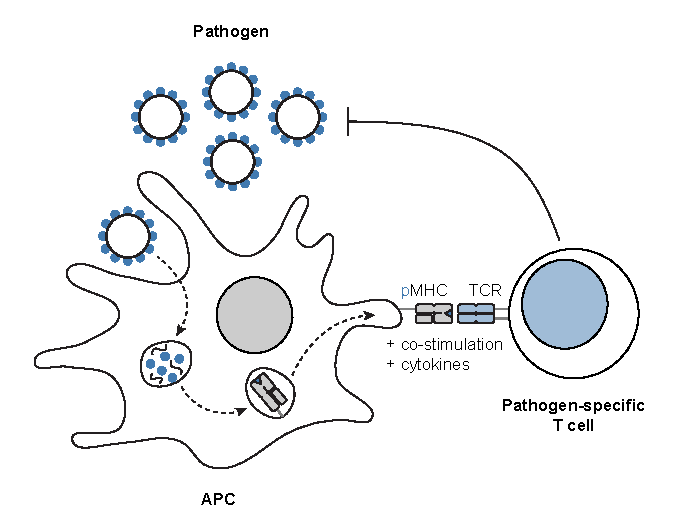
\includegraphics[width=0.64\textwidth]{Figures/intro/fig1_TcellActivation.pdf}
    \caption[Overview of T cell activation via antigen recognition]{\captiontitle{Overview of T cell activation via antigen recognition.} Antigen presenting cells (APCs) phagocytose pathogens and degrade them via proteolytic pathways. Peptide fragments derived from proteins/antigens of the processed pathogen are then coupled to MHC molecules to form peptide-MHC (pMHC) pairs, which are then shuttled to the APC surface. The binding of specific T cell receptors (TCRs) to these pMHC ligands expressed on APCs then trigger, in the presence of co-stimulatory molecules and cytokines produced by APCs, T cell activation and proliferation needed for pathogen control.}
    \label{fig:intro_TcellActivation}
\end{figure}

At this stage, it should be noted that there are two main forms of MHC that we will consider\footnote{Other, non-antigen presenting classes of MHC exist but will not be covered here; for reviews see~\cite{colten1984expression,gruen2001human}.}: they are MHC class I (MHCI), recognized by CD8\pos{} T cells and presenting peptides between 8-15 but usually 9 amino acids long~\cite{trolle2016length,meydan2013prediction}, and MHC class II (MHCII), recognized by CD4\pos{} T cells~\cite{rock2016present} and presenting longer peptides up to 30 amino acids in length~\cite{meydan2013prediction}. The expression of MHCII is restricted to APCs (including dendritic cells, macrophages, and B cells), while all nucleated cells in the body express MHCI~\cite{hewitt2003mhc,van2011expression,rock2016present}. When a cell is infected by an intracellular pathogen, its cellular machinery will conjugate pathogen-derived peptides to MHCI, thus flagging itself for elimination by cytotoxic CD8\pos{} T cells~\cite{rock2016present}.

The importance of the TCR for adaptive immunity cannot be overstated, as the ability of T cells to play out their roles rely crucially on this initial TCR:pMHC interaction. TCRs thus act as the ``eyes'' of the adaptive immune system; only those TCRs that can bind to the pathogen-specific pMHC with adequate strength (in other words, with sufficient ``reactivity'') will become activated and initiate a targeted response to that pathogen. What exactly is meant, from a functional standpoint, by a TCR being ``specific'' for a given pMHC (termed its ``cognate'' pMHC) will be the focus of the next section.

%%%%%%%%%%%%%%%%%%%%%%%%%%%%%%%%%%%%%%%%%%%%%%%%%%%%
\subsection{Antigen discrimination -- how T cells ``know'' when to respond}
\label{sec:intro_overview_antigenDiscrimination}

At homeostasis, all nucleated cells in an organism express pMHC where the ``p'' is a peptide derived from endogenous proteins found throughout the body~\cite{hewitt2003mhc,van2011expression,rock2016present}; these are called self-pMHCs, and, under healthy conditions, normal protein processing pathways within cells lead to baseline self-pMHC expression. In fact, both CD4\pos{} and CD8\pos{} T cells need to receive sub-threshold signals from self-pMHC on APCs to survive long-term in the periphery~\cite{takeda1996mhc,brocker1997survival,kirberg1997peripheral,tanchot1997differential}. An apparent dilemma thus arises: given that all TCRs must bind self-pMHC to some extent, how does an activation threshold manifest itself from a continuous range of TCR:pMHC binding strengths, such that a T cell responds only to pathogen-derived \textit{foreign}-pMHC in a specific yet sensitive way? In other words, how do T cells become activated when presented with foreign antigen even at low concentrations (sensitivity) but remain neutral in the presence of constant and abundant self-pMHC (specificity)? Impressively, it has been shown that even a very small number of pMHC molecules is required for T cell activation~\cite{irvine2002direct}, with as few as one single pMHC ligand being sufficient to induce a measurable T cell response~\cite{huang2013single} provided that the TCR is specific for it. Thus, T cells searching for their cognate pMHC ligand is akin to searching for a needle in a haystack, yet they have remarkably evolved to do exactly that.

Our understanding of just how TCRs can effectuate such exquisite discrimination between self and non-self antigens has greatly benefited from mathematical modelling efforts~\cite{feinerman2008quantitative,franccois2016case}. In 1995, Timothy McKeithan proposed a now-famous conceptual model of immune recognition using the ``kinetic proofreading'' (KPR) principle~\cite{mckeithan1995kinetic}. Briefly, this model assumes that a TCR and pMHC must be bound long enough for TCR-associated intracellular molecules to undergo $N$ successive phosphorylation steps (or modifications), and that only at this stage do downstream signaling processes occur leading to T cell activation. An interesting finding of this model is that, if this theoretical number $N$ is large enough, then even small differences in TCR:pMHC binding duration can lead to large differences in the proportion of complexes that can achieve all $N$ modifications (Fig.~\ref{fig:intro_KPR}). Thus, within this KPR framework, the TCR may theoretically achieve sensitivity for pMHC that it is ``specific'' for while remaining tolerant to others. Recently, Tischer and Weiner used optogenetics to specifically modulate how long the TCR remained bound to antigen~\cite{tischer2019light}; consistent with the KPR principle, they showed that tuning the duration of binding indeed generates a sharp threshold of T cell activation.

\begin{figure}[ht]
    \centering
    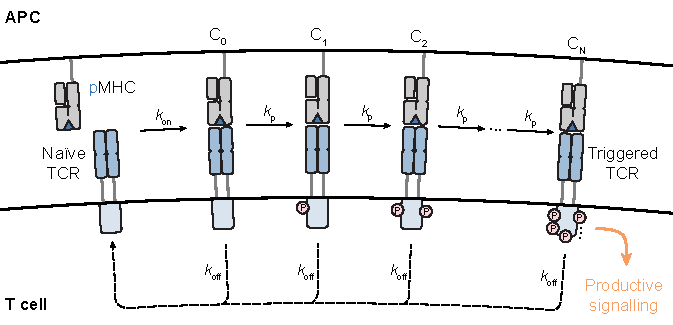
\includegraphics[width=0.64\textwidth]{Figures/intro/fig3_KPR.pdf}
    \caption[Schematic of the kinetic proofreading model for T cell activation]{%
    \textit{Schematic of the kinetic proofreading model for T cell activation}. %
    According to this model, the TCR binds pMHC at a rate $k_{\textup{on}}$ to form a TCR:pMHC complex, $C_0$. While bound, intracellular domains associated with the TCR undergo modifications via phosphorylation at a rate $k_{\textup{p}}$, causing the complex to transition from state $C_i$ to $C_{i+1}$ ($i=0,1,2,..., N-1$), where each transition represents one modification step. Unbinding of the TCR:pMHC complex (at a rate equal to $k_{\textup{off}}$) rapidly reverses these modifications, causing the TCR to revert back to its ``na\"{i}ve'' unbound state. The TCR is assumed to become ``triggered'' only when it undergoes all $N$ modification steps; triggered TCRs then initiate downstream activation and response. The TCR is specific for the pMHC only if the duration of binding is sufficiently long enough to trigger a response. Adapted from~\cite{mckeithan1995kinetic}.}
    \label{fig:intro_KPR}
\end{figure}

In reality, the downstream processes that lead to T cell activation involve a fairly complex biochemical series of events (the details of which lie outside the scope of this thesis; for recent reviews, see~\cite{hwang2020recent,shah2021t}), but importantly $N$ successive modifications proposed by the model can indeed be likened to phosphorylation of immunoreceptor tyrosine-based activation motif (ITAM) sites on the cytoplasmic molecules that complex with the TCR and that are responsible for downstream signal transduction~\cite{vstefanova2003tcr,love2010itam}. Subsequent studies have built upon the KPR principle to incorporate additional aspects of TCR signalling downstream. For example, Altan-Bonnet and Germain developed a detailed biochemical model showing that a combination of positive and negative feedback loops could better achieve sensitivity and specificity for its ligand~\cite{altan2005modeling}. Fran\c{c}ois et al. later showed that even a very simple, phenotypic model incorporating negative regulation to the KPR scheme can reproduce the speed, specificity, and sensitivity required for TCR antigen discrimination, even for smaller numbers of modification steps~\cite{franccois2013phenotypic}.

Other studies have used modelling to suggest additional ways by which TCRs achieve the sensitive and specific recognition of its cognate ligand. In one such case, Dushek and van der Merwe proposed that pMHC ``rebinding'' within the kinetic proofreading scheme can improve antigen discrimination by T cells, for example by inducing the formation TCR nanoclusters  on the T cell surface in such a way that the pMHC is more likely to rebind TCRs as a function of nanocluster size~\cite{dushek2014induced}. In another model, Ganti et al. argue using principles derived from information theory that spatial localization of feedback signals relative to the TCR plays a role, postulating that early negative feedback in physical proximity to the TCR are important for sensitive antigen discrimination, while more distal, late positive feedback serves the purpose of signal amplification post-discrimination~\cite{ganti2020t}.

%%%%%%%%%%%%%%%%%%%%%%%%%%%%%%%%%%%%%%%%%%%%%%%%%%%%
\subsection{T cell proliferation -- raising an army}
\label{sec:intro_overview_proliferation}

Upon interaction with an APC bearing its cognate pMHC, the newly-activated T cell must undergo several rounds of division. The result is exponential growth, with final numbers of activated T cells expanded by several orders of magnitude relative to the number of pre-activated, or ``na\"{i}ve'', T cell precursors. For example, in the case of T cells specific for lymphocytic choriomeningitis virus (LCMV)\footnote{In particular, this study quantified GP$_{33}$-specific CD8\pos{} T cells; these are T cells whose TCRs bind MHC conjugated to a peptide fragment derived from the LCMV viral glycoprotein (GP), starting from position 33 of the GP amino acid sequence up to position 41.}, it was determined that 100-200 na\"{i}ve precursors in mice expand to a staggering $\sim$10 million cells one week post-infection~\cite{blattman2002estimating}. This process of antigen-driven T cell proliferation of a single T cell population has been mathematically described by de Boer and Perelson in 1995~\cite{de1995towards}, who, from a simple kinetic scheme of T cell binding to antigen, derived the following equation:
%
\begin{equation}
    \dv{T}{t} = \sigma + \rho \, T \frac{P}{P + \flatfrac{1}{K} + T} - \delta \, T.
    \label{eq:intro_deboer1995}
\end{equation}
%
Here, $T$ denotes the number of T cells, while $\dv*{T}{t}$ represents the rate of change of this number with respect to time. The term $\sigma$ represents a constant influx of new na\"{i}ve T cell precursors from the thymus, while $\delta$ represents the \textit{per capita} death (i.e., turnover) rate of T cells. The middle term represents the effect of T cell division in the presence of antigen at a concentration $P$, with a maximum \textit{per capita} proliferation rate $\rho$ with the quantity $K$ representing the overall strength of binding of the T cell with the APC -- this parameter is also called T cell ``avidity'' (see Section~\ref{sec:intro_affinity_TcellAvidity}).

This model, while simple and with only a few parameters, provides important insight into key features of T cell replication. First note that, in the absence of cognate pMHC (i.e., when $P=0$), a steady-state level of precursor T cells is reached when $T = \flatfrac{\sigma}{\delta}$; this is obtained by setting Eq.~\eqref{eq:intro_deboer1995} to 0 and solving for $T$, and represents the number antigen-specific T cells at homeostasis (e.g., the 100-200 LCMV precursors). Upon introduction of pathogen, when $P$ is large and $T$ is still small, exponential growth in the number of T cells is observed, hence the number of antigen-specific T cells may grow to very large numbers (e.g., to the 10 million observed a week post-infection with LCMV). Furthermore, the function representing T cell proliferation saturates at high concentrations of cognate pMHC, eventually plateauing at an upper-bound determined by $\rho$. Finally, the additional $T$ term in the denominator represents competition for antigen binding sites between T cells; it becomes important when multiple clones of T cells are considered simultaneously, as it prevents the T cell population in the model from growing unboundedly.

This formalism for T cell proliferation has since been adapted for use in many other population models of effector T cells in various contexts, including those presented in~\cite{de1998target,khadra2009role,khadra2011investigating,conway2015post,mayer2019regulation} developed over a period spanning nearly 30 years. Importantly, this formalism describing T cell expansion in the presence of cognate antigen is adapted in our own models presented in Chapters~\ref{sec:Tr1}-\ref{sec:VE} of this thesis.

%%%%%%%%%%%%%%%%%%%%%%%%%%%%%%%%%%%%%%%%%%%%%%%%%%%%
\subsection{The generation of TCR repertoire diversity}
\label{sec:intro_overview_TCRdiversification}

Conservative estimates put the number of potential antigens that an organism could theoretically encounter throughout its life on the order of trillions, though the true number could very well be several orders of magnitude more than even this~\cite{mason1998very,yates2014theories}. Given this enormous variety, a mechanism needs to be put in place to generate a sufficient number of unique TCRs so as to be able to cover the sheer breadth of potential antigens that the host may encounter.

Each T cell expresses many copies (on the order of $10^4$) of a unique TCR on its surface~\cite{labrecque2001much}. The collection of all T cells bearing the same TCR is called a T cell clonotype, while the collection of all unique TCRs within an organism is termed its TCR ``repertoire''. Structurally, the TCR is a heterodimer, with most circulating T cells being formed from a TCR\textalpha{} and a TCR\textbeta{} chain; these are termed \textalpha{}\textbeta{}~T cells.\footnote{A small subset of circulating T cells, present at a frequency of $\sim$1-5\% in adult humans and mice~\cite{lanier1988structural,groh1989human}, are instead formed from a \textgamma{}- and a \textdelta{}-chain. These \textgamma{}\textdelta{}~T cells are present at higher frequencies in the skin and gut and, while interesting in their own right, will not be covered in this thesis -- for a review of \textgamma{}\textdelta{}~T cells and their function, see~\cite{vantourout2013six}.} Early estimation of the number of unique \textalpha{}\textbeta{}~T cell clonotypes determined a lower bound of 25 million unique TCRs in the human body, with true diversity certain to exceed this figure~\cite{arstila1999direct}. The number of protein-coding genes in the human genome, on the other hand, is only about 20 thousand~\cite{salzberg2018open,piovesan2019human}. Thus, there cannot be a one-to-one correspondence between a gene and a unique TCR\textalpha{} or TCR\textbeta{} chain. Instead, jawed vertebrates have evolved a clever process to generate large T and B lymphocyte receptor diversities, called V(D)J recombination~\cite{litman2010origins}.

The T and B cell antigen receptors coded by the germline DNA (i.e., the inherited version of those genes) are non-functional prior to lymphocyte development; instead, they are composed of many V and J segments, with the germline TCR\textbeta{} gene also containing 2 additional D segments in the case of T cells~\cite{litman2010origins,schatz2011recombination}. During T cell development in the thymus, recombination-activating gene (RAG) protein complexes mediate the semi-random combination of these V and J (for the TCR\textalpha{} chain), or V, D, and J (for the TCR\textbeta{} chain), segments~\cite{schatz2011recombination,robins2010overlap}, generating massive diversity from the sheer number of possible combinations of these segments. Additionally, during RAG-mediated joining of each pair of segments, a unique DNA polymerase called terminal deoxynucleotidyl transferase (henceforth referred to as TdT) inserts an average of 2 to 5 non-templated (simply put: random) nucleotides, or ``N-nucleotides'', into the junctions between these segments~\cite{schatz2011recombination,mickelsen1999modulation}\footnote{The functional role of N-diversification by TdT will be investigated further in Chapters~\ref{sec:AvC} and~\ref{sec:VE}.}. Finally, pairing of the new TCR\textbeta{} chain (which undergoes recombination first) to the new TCR\textalpha{} chain to form the TCR heterodimer further increases the number of possible TCRs, with at least 25 TCRs, on average, sharing the same TCR\textbeta{} chain while differing via distinct TCR\textalpha{} chains~\cite{arstila1999direct}. The mechanisms of TCR repertoire diversification are summarized in Fig.~\ref{fig:intro_TCRdiversity}. Together, these processes combined were estimated to generate an astounding $10^{15}$ to $10^{20}$ unique TCRs~\cite{davis1988t,zarnitsyna2013estimating}; to put into context just how massive this number is, the number of grains of sand in all the beaches and deserts on Earth, approximately 7.5\E{18}~\cite{blatner2012spectrums}, falls squarely within this range.

\begin{figure}[ht]
    \centering
    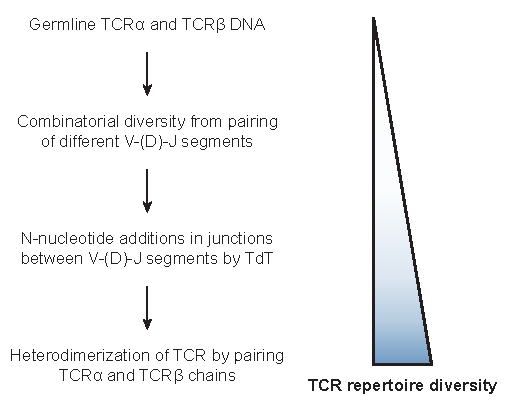
\includegraphics[width=0.48\textwidth]{Figures/intro/fig2_TCRdiversity.pdf}
    \caption[Summary of TCR repertoire diversification]{%
    \textit{Summary of TCR repertoire diversification}. %
    Combinatorial diversity is achieved by random joining of V, (D,) and J segments recombination, N-nucleotide addition, and heterodimerization of TCR\textalpha{} and TCR\textbeta{} chains.}
    \label{fig:intro_TCRdiversity}
\end{figure}

The ``realized'' repertoire diversity of T cells, however, is certainly smaller than this theoretical maximum. For one, there are about 400 billion T cells throughout the human body~\cite{jenkins2009composition}; $10^{15}$ T cells, on the other hand, would weigh about half a metric tonne~\cite{lythe2016many}. Extrapolating, $10^{20}$ T cells would weigh around 50,000 tonnes, more than four times the weight of the Eiffel Tower. Second, there exist many T cell clonotypes composed of multiple T cells with identical TCRs~\cite{robins2009comprehensive,quigley2010convergent,zarnitsyna2013estimating,qi2014diversity,de2020naive}. Third, V(D)J recombination is not totally random, as it is known that there are intrinsic biases in segment usage and N-nucleotide additions by TdT~\cite{robins2010overlap,murugan2012statistical}, and redundancies in protein encoding would mean that different genetic sequences could converge to the same TCR protein structure~\cite{quigley2010convergent}. Fourth, not all rearranged TCRs will live to see the light of day owing to harsh selection processes in the thymus. Specifically, once the developing T lymphocyte has successfully rearranged its TCR, that new TCR must be tested for its ability to bind self-pMHC sufficiently (ensuring that the TCR is functional and useful) but not excessively (to prevent autoimmune responses). The processes of positive and negative selection in the thymus, respectively, are the mechanisms that ensure these two conditions are met~\cite{yates2014theories,klein2014positive,kondo2019thymus}. Together, these checkpoints purge about 95\% or more of T cells before they can become fully fledged mature na\"{i}ve T cells in the periphery~\cite{kyewski2006central}.

Estimates from TCR sequencing data on the realized TCR diversity in adult humans range from $10^7$ to $10^8$ unique TCR clonotypes~\cite{robins2009comprehensive,qi2014diversity,de2020naive}. Incidentally, there are many technical challenges involved in measuring realized TCR repertoire diversity across all T cells of the body~\cite{zarnitsyna2013estimating,mora2019many} which involves extrapolation of data obtained from a comparatively small subset of all TCRs (a truly non-trivial task). Stochastic models have therefore been used to infer T cell clonotype distributions, and consequently the number of T cell clones, based on homeostatic processes such as thymic input, division, cell death, and competition for self-pMHC~\cite{desponds2016fluctuating,lythe2016many,mora2019many}. In particular, Lythe et al. used such a model to propose that the number of T cell clonotypes may be much higher than previous estimates, finding that this number may only be about 10-fold lower than the total number of T cells~\cite{lythe2016many} in the periphery, i.e., on the order of $\sim$10 billion ($10^{10}$) in humans.

%%%%%%%%%%%%%%%%%%%%%%%%%%%%%%%%%%%%%%%%%%%%%%%%%%%%
\subsection{Summary and highlights}

The concepts of TCR diversification, antigen recognition/discrimination, and pMHC binding strengths have important implications for T cell responses, and thus for proper immune function. At one extreme, failure of T cells to discriminate between self- and foreign-pMHC can lead to the development of autoimmune disorders. What mechanisms exist to prevent their manifestation, and under what conditions these mechanisms may fail, will be discussed in Section~\ref{sec:intro_autoimmunity}. At the other extreme, failure of T cells to recognize and respond to foreign pathogens can lead to immunodeficiency and immune escape. The mechanisms used by pathogens to evade T cell recognition will be discussed in Section~\ref{sec:intro_immuneEscape}. Between these two extremes, T cells recognize foreign-pMHC with varying degrees of sensitivity lying within a continuum of binding strengths. How this continuum is defined, and how it may shape the anti-microbial T cell response, will be discussed in Section~\ref{sec:intro_affinity}.

%%%%%%%%%%%%%%%%%%%%%%%%%%%%%%%%%%%%%%%%%%%%%%%%%%%%
%%%%%%%%%%%%%%%%%%%%%%%%%%%%%%%%%%%%%%%%%%%%%%%%%%%%

\section{T cell tolerance and autoimmunity}
\label{sec:intro_autoimmunity}

As mentioned in Section~\ref{sec:intro_overview_antigenDiscrimination}, self-pMHC is present throughout the entire body. The question becomes: how are T cells, which rearrange their TCR and undergo selection processes in the thymus, supposed to be trained not to become activated by self-pMHC in the periphery? Training T cells to remain ``tolerant'' to self is critical, as TCR signal strengths resulting from interactions with self-pMHC that are too strong can lead to T cell activation and immune-driven destruction of healthy endogenous tissue --  a hallmark of autoimmunity. Indeed, autoimmune disorders, like any adaptive immune response, are believed to be T cell mediated; examples where this is known include, but are not limited to, type 1 diabetes mellitus, rheumatoid arthritis, multiple sclerosis, Hashimoto's disease, autoimmune hepatitis, inflammatory bowel disease, and systemic lupus erythematosus~\cite{giwa2020current,weyand2020immunometabolism,liu2022autoreactive,chistiakov2005immunogenetics,sirbe2021pathogenesis,imam2018effector,sharabi2020t}.

In all cases, autoimmune T cell responses arise in contexts where the mechanisms of self-tolerance fail. Broadly, the checkpoints in place to prevent autoimmunity belong to one of two categories: central tolerance, or peripheral tolerance. What these are, and how they work to circumvent the development of autoimmune disorders via autoreactive T cells will be the focus of this section. Note that the concept of T cell tolerance is broad and can extend beyond the context of self-antigens to include, for example, tolerance to commensal microbes that constitute the symbiotic microbiome~\cite{nutsch2012t}, or exhaustion in the context of chronic infections or cancer~\cite{schietinger2014tolerance} (a concept that will be revisited in Section~\ref{sec:intro_immuneEscape_mechanisms}). The remainder of this section, however, will focus specifically on the establishment (or failure) of tolerance to self in the context of autoimmunity.

%%%%%%%%%%%%%%%%%%%%%%%%%%%%%%%%%%%%%%%%%%%%%%%%%%%%
\subsection{Central tolerance -- the role of negative selection}
\label{sec:intro_autoimmunity_centralTolerance}

Central tolerance comprises the set of processes during T cell development within the thymus that aim to eliminate autoreactive T cells whose rearranged TCRs bind self-pMHC too strongly (thus having the potential to become activated in the periphery in response to antigens derived from the host's own tissue). This process is termed negative selection, and was touched upon briefly in Section~\ref{sec:intro_overview_TCRdiversification}.  After developing T cells have undergone V(D)J recombination for both chains of their TCR and have passed through positive selection in the cortical region of the thymus, they migrate to the thymic medulla~\cite{takahama2006journey,love2011signal}. There, a specialized subset of medullary thymic epithelial cells (mTECs), together with dendritic cells (a professional APC) and thymus-resident B cells, will present a large library of self-antigens derived from proteins expressed throughout the entire body~\cite{klein2014positive,takahama2006journey,love2011signal,castaneda2021multifaceted}. While some of these self-antigens may be found ubiquitously throughout the body (since they are derived from proteins expressed in many or all cell types), others may only be expressed in very specific organs and are hence referred to as ``tissue-restricted'' antigens (TRAs)~\cite{kyewski2006central,kondo2019thymus}.

If a T cell, via its TCRs, binds too strongly to self-pMHC in the thymus that it could potentially re-encounter in the periphery, this leads to one of two potential outcomes~\cite{kondo2019thymus}. In the first case, the T cell is deleted by apoptosis (i.e., programmed cell death) and thus prevented from escaping the thymus and becoming part of the mature na\"{i}ve T cell pool. In the second, however, the T cell is instead destined to become a regulatory T cell or Treg (specifically, a ``natural'' Treg, in contrast to ``induced'' Tregs which will be discussed in Section~\ref{sec:intro_autoimmunity_Tregs}). Tregs, as mentioned in Section~\ref{sec:intro_overview_Tcells}, differ from conventional T cells in that they instead primarily play an immunosuppressive (as opposed to a pro-inflammatory) role. The result is thus an immunosuppressive T cell that binds self-pMHC more strongly, on average, than circulating conventional T cells~\cite{tanaka2010graded,killebrew2011self,moran2011t,li2016t}. Which of these two fates (apoptosis or diversion to the Treg lineage) awaits a given autoreactive T cell in the thymus is still not completely understood, though this is likely a result of multiple factors. For one, it was shown that self-pMHC expression patterns in the thymus can influence this outcome, where higher expression levels favour clonal deletion while lower expression levels favour the production of Tregs~\cite{malhotra2016tolerance}. Additionally, there is evidence to suggest that intrinsic properties of the TCR itself might play a role, given that the genetic sequences that make up the TCRs of conventional vs. regulatory T cells were shown to be distinct (though with some degree of overlap)~\cite{hsieh2004recognition,wong2007adaptation,savage2020regulatory}.

The ability for mTECs to express pMHC that might only be found, for example, in the kidney or in the pancreas, is known as promiscuous gene expression and is key to establishing central tolerance. This function is largely (though not exclusively) mediated by a unique transcription factor known as autoimmune regulator (AIRE)~\cite{derbinski2005promiscuous,kyewski2006central}. Indeed, people with mutations in the gene encoding AIRE, leading to deficiency in AIRE expression, present with severe multiple-organ autoimmunity~\cite{betterle1998autoimmune,anderson2005cellular,besnard2021aire}, thus highlighting the crucial role of central tolerance mechanisms in preventing autoimmune disorders. 


%%%%%%%%%%%%%%%%%%%%%%%%%%%%%%%%%%%%%%%%%%%%%%%%%%%%
\subsection{Peripheral tolerance -- ignorance, anergy, and regulation}
\label{sec:intro_autoimmunity_peripheralTolerance}

Central tolerance in the thymus allows for the detection and deletion of autoreactive T cells before they have the opportunity to encounter their cognate antigen, derived from self, in the periphery. However, it has been established that central tolerance is a fairly incomplete process, and that a sizeable fraction of autoreactive T cells ($\sim$1/3) do escape negative selection to become part of the mature na\"{i}ve T cell repertoire~\cite{bouneaud2000impact,gallegos2006central,eltanbouly2021rethinking}. Therefore, while necessary, central tolerance alone is not sufficient for curtailing autoimmune responses. Accordingly, additional mechanisms must be put in place in order to prevent the development of autoimmune disease; these additional mechanisms fall under the umbrella of peripheral tolerance.

T cell ignorance is perhaps the first facet of peripheral tolerance specifically keeping autoreactive T cells in check~\cite{salaman2020breakdown,eltanbouly2021rethinking}. Conventional na\"{i}ve CD4\pos{} and CD8\pos{} T cells, including those that are autoreactive, exit the thymus in a quiescent state~\cite{chapman2020metabolic}; as described in Section~\ref{sec:intro_overview_antigenDiscrimination}, these T cells only exit quiescence if their TCR comes into contact with their cognate pMHC and the stability and duration of this interaction is sufficient to trigger T cell activation. However, perhaps due to autoreactive T cells having TCRs that bind their cognate self-antigen less strongly~\cite{zehn2006t,leube2023single} in combination with low abundance of (and/or restricted access of these T cells to) their cognate self-antigens~\cite{kurts1999cd8,eltanbouly2021rethinking}, they may fail to become activated in the periphery (Fig.~\ref{fig:intro_peripheralTolerance}A). 

\begin{figure}
    \centering
    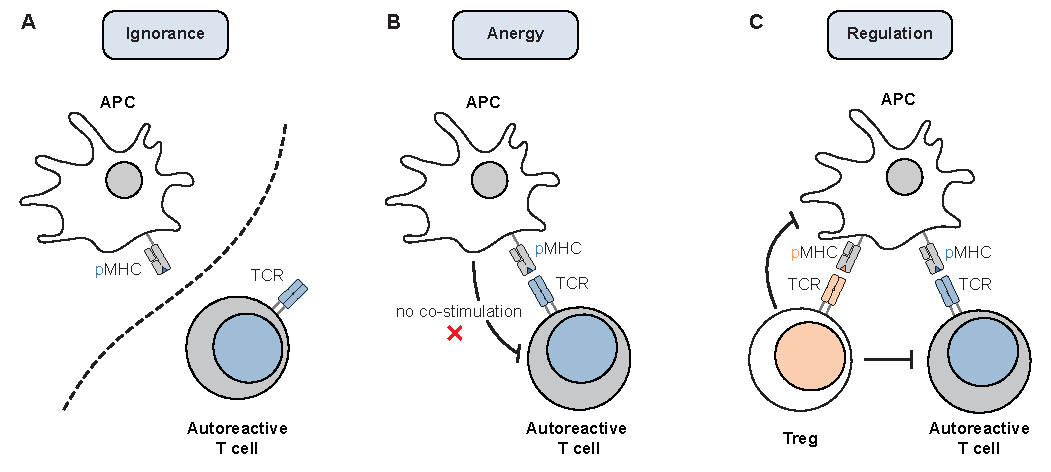
\includegraphics[width=\textwidth]{Figures/intro/fig4_peripheralTolerance.pdf}
    \caption[Summary of peripheral tolerance mechanisms]{%
    \textit{Summary of peripheral tolerance mechanisms}. %
    \secbfcolor{(A)}~T cell ignorance occurs when an autoreactive T cell fails to activate in the periphery, owing to restricted access of its TCR to its cognate pMHC on APCs, and/or no/low self-antigen abundance in conjunction with low TCR:pMHC binding strengths. %
    %
    \secbfcolor{(B)}~T cell anergy (hyporesponsiveness) is induced upon TCR:pMHC engagement in the absence of co-stimulatory signals from the APC. %
    %
    \secbfcolor{(C)}~Regulatory T cells (Tregs) use a number of mechanisms to suppress autoreactive T cell activation, acting both directly on those T cells or by impairing the ability of APCs to activate them.}
    \label{fig:intro_peripheralTolerance}
\end{figure}

The next line of defence in the peripheral tolerance arsenal is the induction of autoreactive T cell anergy. Briefly, anergy is defined as a long-lasting hyporesponsive state following cognate antigen encounter~\cite{schwartz1989t,schwartz2003t,appleman2003t,eltanbouly2021rethinking}. As mentioned in Section~\ref{sec:intro_overview_antigenRecognition}, the TCR:pMHC interaction is necessary but not sufficient to induce T cell activation and proliferation~\cite{lafferty1978immunological,mueller1989accessory}. In fact, in the absence of co-stimulation through accessory surface proteins on the APC (e.g., B7-1 or B7-2) engaging their ligands on the T cell (e.g., CD28), T cell activation fails and the T cell is rendered unresponsive even to subsequent antigen stimulation~\cite{ragazzo2001costimulation,wells2001signaling}. It should be noted that there is considerable phenotypic diversity with regard to transcriptional states in anergic T cells (reviewed in~\cite{valdor2013induction}) as well as different molecular mechanisms that can induce distinct forms of T cell anergy~\cite{wells2001signaling}. In any case, the bottom line is that these autoreactive T cells are prevented from becoming fully-fledged effector T cells, thus sparing the organism from damaging autoimmune responses (Fig.~\ref{fig:intro_peripheralTolerance}B).

Another crucial contributor to the establishment of peripheral tolerance, and the focus of the remainder of this section, is the regulatory T cell (Treg). Although these immunosuppressive T cells can exert their effect in several distinct ways~\cite{sakaguchi2008regulatory,shevyrev2020treg}, it was shown that, like conventional T cells, many Treg functions rely on the ability of their TCR to engage self-pMHC in the periphery~\cite{levine2014continuous,vahl2014continuous,schmidt2015regulatory}. In addition to serving the important role of peripheral tolerance to self-antigens, Tregs also induce tolerance to microbiome-derived, food-derived, and fetus-derived antigens, and are involved in tissue regeneration post-injury~\cite{xu2018c,zhang2001activation,burt2013fetal,shevyrev2020treg}. An overview of different types of regulatory T cells, as well as a summary of ways in which these Tregs exert their immunosuppressive effects in the context of peripheral tolerance to self-antigens, will be provided in the next section.

%%%%%%%%%%%%%%%%%%%%%%%%%%%%%%%%%%%%%%%%%%%%%%%%%%%%
\subsection{Regulatory T cells -- subsets and mechanisms of action}
\label{sec:intro_autoimmunity_Tregs}

Typically, the name Treg is used interchangeably with CD25\pos{} CD4\pos{} T cells expressing FOXP3, the master transcriptional regulator of Treg cell development and function. These can be further divided into natural Tregs (nTregs) that already express FOXP3 and possess an immunoregulatory phenotype upon egress from the thymus, vs. induced Tregs (iTregs) that begin as conventional CD25\neg{}~CD4\pos{} T cells and acquire FOXP3 expression and immunoregulatory potential in the periphery upon antigenic stimulation in the presence of the cytokine TGF-\textbeta{}~\cite{chen2003conversion,sakaguchi2008regulatory}. Mutations in the gene encoding FOXP3, resulting in dysfunction of these Tregs, is the underlying cause of IPEX (immune dysregulation, polyendocrinopathy, enteropathy, X-linked), a rare and severe multi-organ autoimmune disorder~\cite{gambineri2003immune,agakidis2019immune}; this affliction highlights just how important Treg function is for maintaining peripheral tolerance and preventing autoimmunity.

FOXP3\pos{} CD25\pos{} Tregs can exert their immunosuppressive properties in a number of ways. First, by engaging self-pMHC expressed on APCs through their TCR in conjunction with high expression levels of adhesion molecules on the Treg cell surface, they may spatially outcompete autoreactive T cells for binding sites on the APC, thus prevent the latter from becoming activated~\cite{tadokoro2006regulatory,tang2008FOXP3+}. Second, Tregs can act as a sink for the cytokine IL-2, sequestering it from effector T cells and inducing cytokine-deprivation mediated apoptosis in these autoreactive cells~\cite{pandiyan2007cd4+}. Third, they can modify APC function through the release of immunosuppressive cytokines, such as IL-10 and TGF\textbeta{}, thus inhibiting their capacity to present self-pMHC to, and prime, autoreactive T cells. Furthermore, they can impair the ability for APCs to deliver co-stimulatory signals to effector T cells by physically ripping co-stimulatory molecules B7-1 and B7-2 off the APC surface in a process known as trogocytosis~\cite{tekguc2021treg}, which depends on the expression of CTLA-4 on the Treg cell surface (Fig.~\ref{fig:intro_peripheralTolerance}C). Impressively, this list is still non-exhaustive, and additional mechanisms of immunosuppression by Tregs have been described (reviewed in~\cite{sakaguchi2008regulatory,shevyrev2020treg}).

Unfortunately, by using the word Treg to specifically refer to FOXP3\pos{} CD25\pos{} CD4\pos{} Tregs, other -- perhaps underappreciated -- types of regulatory T cells are left out. In particular, type 1 regulatory T cells (henceforth referred to as Tr1s), a separate subset of induced CD4\pos{} Tregs that are CD25\neg{} FOXP3\neg{}, have important commonalities with the more ``traditional'' FOXP3\pos{} Tregs~\cite{sakaguchi2008regulatory,freeborn2022type}. For example, they too secrete TGF-\textbeta{} and large amounts of IL-10 upon cognate antigen recognition~\cite{bacchetta1994high,groux1997cd4+}. Additionally, like their FOXP3\pos{} counterparts, Tr1s comparably display CTLA-4-dependent immunosuppressive functions~\cite{chen2021alloantigen}. Recent work has suggested that the precursors of these Tr1 cells are antigen-experienced anergic CD4\pos{} T cells that, upon re-encounter of its cognate antigen, is diverted to the Tr1 lineage~\cite{thomann2021conversion}. Impressively, selective expansion of self-pMHC specific Tr1 cells in experimental autoimmune mice can, in some cases, blunt the progression and even reverse the effects of autoimmune destruction~\cite{clemente2016expanding,umeshappa2019suppression,umeshappa2020ubiquitous}. However, this therapeutic intervention is not always effective, and uncovering the mechanisms driving treatment success will be the goal of our work in Chapter~\ref{sec:Tr1}. It should also be noted that other subsets of T cells with immunoregulatory potential have been described, such as CD4\pos{} T-helper type 3 (Th3) cells~\cite{chen1994regulatory,krop2020regulatory} and regulatory CD8\pos{} T cells~\cite{mishra2021cd8+}, though these will not be discussed here.

%%%%%%%%%%%%%%%%%%%%%%%%%%%%%%%%%%%%%%%%%%%%%%%%%%%%
\subsection{Central vs. peripheral tolerance -- why both?}
\label{sec:intro_autoimmunity_whyCentralAndPeripheral}

On the surface, it may not be obvious why vertebrates have evolved the need for both central and peripheral tolerance mechanisms. One might ask: why is central tolerance as incomplete as it is; in other words, why have we not evolved an (even more) rigorous process of negative selection that completely purges the peripheral TCR repertoire of any and all autoreactive T cells? As it stands, there is no definitive answer to this question, but it has been suggested that the $\sim$1/3 of autoreactive T cells (with low self-pMHC binding strength) that escape central tolerance may be important for cross-reacting to foreign antigens with higher binding strengths~\cite{sandberg2000t,bouneaud2000impact,this2021strength}. Indeed, it should be appreciated that the line between self- and foreign-pMHC, from the perspective of the TCR, is quite blurred, with a potentially high degree of overlap (``degeneracy'') between the two~\cite{calis2012degenerate}. Thus, one hypothesis is that complete purging of autoreactive TCRs via negative tolerance would exacerbate ``holes'' in the TCR repertoire and result in impaired pathogen recognition~\cite{this2021strength} (this relationship between TCR repertoire diversity and pathogen control will be examined in more detail in Chapters~\ref{sec:AvC} and~\ref{sec:VE}).

Given that these autoreactive T cells do partially bypass negative selection in the thymus, peripheral tolerance must necessarily complement it. Mathematical modelling has helped us to functionally understand how central and peripheral tolerance, together, might prevent autoimmunity while preserving the host's ability to respond to foreign pathogens~\cite{borghans1998crossreactivity,borghans1999specific,jaberi2014autoimmune}. For example, Khailaie et al. developed an ODE model of effector and regulatory T cell populations coupled to IL-2 dynamics (which Tregs sequester from effector T cells as a mode of suppression) to show that adequate Treg/effector T cell ratios, together with a lower number of effector T cell precursors with sufficiently high antigen stimulation thresholds (e.g. due to low self-pMHC binding strength), can lead to sub-critical stimulation and no response (e.g., no autoimmunity)~\cite{khailaie2013mathematical}. In contrast, greater effector T cell precursor numbers with lower antigen stimulation thresholds (i.e., higher pMHC binding strengths) can overcome regulatory T cell mediated immunosuppression and carry out an immune response, as would be required in the event of an infection with a foreign pathogen.

In contrast to the presumably lower self-pMHC binding strength of autoreactive T cells, recall that Tregs (or at least FOXP3\pos{} CD25\pos{} nTregs that develop in the thymus) bind self-pMHC more strongly through their TCR, on average. To further study the relationship between self-pMHC binding strengths of effector T cells vs. Tregs and their role on autoimmune disease onset, Jaberi-Douraki et al.~\cite{jaberi2015continuum} developed an integro-differential equation model where these quantities were defined along a continuum in the context of type 1 diabetes. Their model results predict that an imbalance in the ratio of Tregs to effector T cells specifically at high self-pMHC binding strengths drives peripheral tolerance failure and progression to diabetes. These findings provide further support regarding the benefit of preferential deletion, or diversion to the Treg lineage, of autoreactive T cell clones with high self-pMHC binding strength at the level of the thymus.

%%%%%%%%%%%%%%%%%%%%%%%%%%%%%%%%%%%%%%%%%%%%%%%%%%%%
\subsection{Summary and highlights}

Central and peripheral tolerance mechanisms are necessary to prevent the development of autoimmune disorders. Regulatory T cells, key executors of peripheral tolerance, require self-pMHC interactions through their TCR in order to perform most of their immunosuppressive functions. When tolerance fails, autoimmunity is manifested via autoreactive T cell-mediated destruction of endogenous tissue. Importantly, nonlinear interactions between autoreactive and regulatory T cells can drive the development, or suppression, of autoimmunity. Of note, pMHC specificity of Tr1 cells, a regulatory T cell subset that can be therapeutically expanded in an antigen-specific manner, will impact whether autoimmune disorders in experimental mouse models can be reversed or not~\cite{umeshappa2020ubiquitous}; however, the outcomes of these experimental treatments could not be easily explained in more complex settings (see preface to Chapter~\ref{sec:Tr1}). Thus, in Chapter~\ref{sec:Tr1}, we will use a cellular population model to study how these Tr1 cells shape immunosuppression of tissue-restricted autoimmune disorders as a function of their antigen specificity.



%%%%%%%%%%%%%%%%%%%%%%%%%%%%%%%%%%%%%%%%%%%%%%%%%%%%
%%%%%%%%%%%%%%%%%%%%%%%%%%%%%%%%%%%%%%%%%%%%%%%%%%%%
\section{T cell antigen reactivity}
\label{sec:intro_affinity}

The processes of V(D)J recombination, together with positive and negative selection checkpoints in the thymus (described in Sections~\ref{sec:intro_overview_TCRdiversification} and~\ref{sec:intro_autoimmunity_centralTolerance}), determine the peripheral TCR repertoire of an organism. Positive selection assigns a lower bound of binding strengths to self-pMHC that T cells, through their TCR, may possess; this ensures functional sub-threshold TCR signalling required for T cell homeostasis. Conversely, negative selection purges T cells with binding strengths to self-pMHC that are too high, thus setting the upper bound of self-pMHC reactivity. Importantly, the result is a repertoire composed of a large number of TCRs that bind pMHC along a continuum of binding strengths within these limits set by thymic selection processes.

TCR signal strengths acquired through interactions with self- or foreign-pMHC have a range of consequences on the T cell response. For example, numerous groups have demonstrated that reactivity to self-pMHC can influence lineage commitment to different CD4\pos{} effector subsets upon foreign antigen encounter~\cite{martin2013highly,van2014t,sood2019differential,rogers2021pre,snook2018tcr,ditoro2018differential,van2016tcr}. The discussion around the strength of interactions between a T cell and an APC bearing its cognate pMHC is often nuanced as there are a number of metrics that describe this strength at multiple scales (and an even larger number of ways with which those quantities are experimentally measured or inferred); these will be discussed in the following sections.

%%%%%%%%%%%%%%%%%%%%%%%%%%%%%%%%%%%%%%%%%%%%%%%%%%%%
\subsection{TCR affinity -- the building block of T cell signal strength (?)}
\label{sec:intro_TCRaffinity}

\begin{figure}[tb]
    \centering
    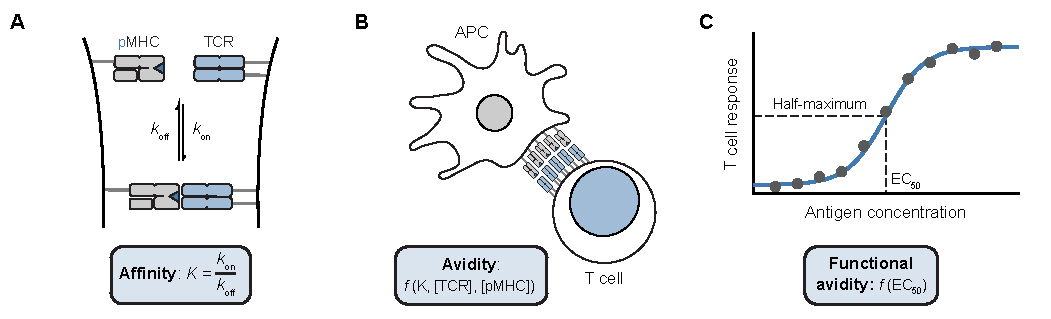
\includegraphics[width=\textwidth]{Figures/intro/fig6_affinityVsAvidity.pdf}
    \caption[Schematic depiction of TCR affinity, T cell avidity, and functional avidity]{%
    \textit{Schematic depiction of TCR affinity, T cell avidity, and functional avidity}. %
    %
    \secbfcolor{(A)}~TCR binding affinity for pMHC, denoted by $K$, is defined as the ratio between binding ($k_{\textup{on}}$) and unbinding ($k_{\textup{off}}$) rates. %
    %
    \secbfcolor{(B)}~T cell avidity is the cumulative binding strength that depends on the binding affinity of TCRs for pMHC, $K$, as well as on the surface densities of TCRs and pMHCs on the T cell and APC, respectively. %
    %
    \secbfcolor{(C)}~The functional avidity of the T cell is its measured sensitivity to pMHC, using readouts such as IFN-\textgamma{} production as a function of antigen concentration. It depends on the TCR:pMHC binding affinity, their respective surface densities, CD4/CD8 co-receptor expression, and other surface and intracellular signalling molecules that together modulate downstream T cell activation. Adapted from~\cite{this2021strength}.}
    \label{fig:intro_affinityVsAvidity}
\end{figure}

The fundamental interaction unit between a T cell and and an APC is the binding of one TCR to one pMHC; the  affinity of the TCR describes the strength of this unitary interaction. In a nutshell, the binding affinity represents the likelihood that a TCR ($T$) and pMHC ($P$) will remain in a bound state ($C$), and can be quantified via the equilibrium constant, $K$, of the following kinetic scheme (Fig.~\ref{fig:intro_affinityVsAvidity}A):
%
\begin{equation}
    \ch{$T + P$ <=>[$k\sb{\textup{on}}$][$k\sb{\textup{off}}$] $C$}.
\end{equation}
%
This equilibrium constant (also called the association constant) is a basic thermodynamic parameter, and is equal to the ratio between the binding and unbinding rates ($k_{\textup{on}}$ and $k_{\textup{off}}$, respectively), i.e., $K = \flatfrac{k_{\textup{on}}}{k_{\textup{off}}}$~\cite{stone2013role,margulies2001tcr}. The magnitudes of these kinetic parameters will be influenced by the TCR sequence, the MHC sequence, and the specific (self or foreign) peptide that is conjugated to the MHC~\cite{this2021strength}. Often, this quantity is given in terms of the dissociation constant, $K_D$~\cite{margulies2001tcr,martinez2015lower}, defined as the reciprocal of the association constant (i.e., $K_D = \flatfrac{1}{K}$).

It should be emphasized that, in reality, the binding affinity of a given TCR:pMHC pair depends on two independent parameters ($k_{\textup{on}}$ and $k_{\textup{off}}$) and each of these rates by themselves can have their own effect on TCR signalling. Indeed, Gálvez et al. showed, using a large collection of previously published T cell activation models based on the kinetic proofreading principle (see Section~\ref{sec:intro_overview_antigenDiscrimination}), that different values of $k_{\textup{on}}$ and $k_{\textup{off}}$ in almost all of these models can produce different outcomes, even if their ratio is fixed~\cite{galvez2019tcr}. It should therefore be borne in mind that, all else being equal, even two TCRs with the same measured affinity for a given pMHC may not necessarily lead to the same T cell response.

To obtain a direct measurement of TCR affinity and its associated kinetic parameters to a given pMHC, techniques such as isothermal titration calorimetry or surface plasmon resonance (SPR) have been used (reviewed in detail in~\cite{piepenbrink2009methods}). With SPR, different T cell clonotypes were found to have dissociation constants $K_D$ ranging from $\sim$0.1~\textmu{}M for high-affinity TCRs, up to the order of $100$~\textmu{}M for low-affinity TCRs~\cite{davis1998ligand,thomas2011human} (an appreciably large range spanning 4 orders of magnitude). These techniques have their share of disadvantages, however, with one being that they measure 3D binding affinities of free-floating, soluble TCRs when in fact TCR interaction with pMHC \textit{in vivo} is confined to 2D space across opposing T cell/APC membranes~\cite{martinez2015lower}. Alternative measures use techniques such as adhesion frequency and thermal fluctuation assays~\cite{huang2010kinetics} or single-molecule microscopy~\cite{huppa2010tcr} to determine binding affinities constrained to more realistic 2D environments; these 2D techniques indeed generate measurements with important differences when compared to their 3D counterparts~\cite{huang2010kinetics,huppa2010tcr,martinez2015lower}. A shortcoming associated with all of these techniques is that they cannot be used to measure affinity across all responding T cell clonotypes in a polyclonal response to a pathogen; rather, they are limited to measuring the affinity of one T cell clone or, at best, of T cell clonotypes with the same pMHC specificity.

%%%%%%%%%%%%%%%%%%%%%%%%%%%%%%%%%%%%%%%%%%%%%%%%%%%%
\subsection{T cell avidity -- a multi-dimensional gauge of pMHC reactivity}
\label{sec:intro_affinity_TcellAvidity}

While TCR affinity (and its corresponding kinetic parameters) certainly impact the strength of interaction between a T cell and an APC, scaling up from the molecular to the cellular level introduces additional layers of complexity. The propensity for T cells as a whole to bind an APC bearing cognate pMHC is termed its \textit{avidity}~\cite{this2021strength}. The magnitude of T cell avidity will depend on the binding affinity of one TCR:pMHC unit, together with the density of TCRs and pMHCs on the surfaces of the T cell and the APC, respectively (Fig.~\ref{fig:intro_affinityVsAvidity}B). Thus, a T cell with a fixed TCR surface density and a fixed binding affinity for a given pMHC may have different avidities for an APC depending on whether it expresses low, or high, levels of that cognate pMHC.

Staining of T cells using multi-valent, fluorescent pMHC compounds, or pMHC tetramers, is frequently used to quantify T cell avidity~\cite{christophersen2020peptide}. Given that the signal intensity will depend directly on the concentration of TCRs on the cell surface~\cite{christophersen2020peptide,wooldridge2009tricks}, pMHC tetramers only provide an indirect measure of its TCR affinity for the pMHC. Furthermore, tetramers have the misfortune of being less sensitive to T cells whose TCRs bind pMHC with low affinity, with one study showing that a large fraction of low-affinity responders are missed by tetramer staining altogether~\cite{andargachew2018cd4}. Furthermore, as with SPR or 2D affinity techniques, \textit{a priori} knowledge of T cell antigen specificity is needed to measure T cell avidity by tetramer staining, and use of tetramers to this effect may leave out important contributions from other T cells that recognize different pathogen-derived pMHC (known as different pMHC ``epitopes'').

The term T cell avidity is sometimes used interchangeably with \textit{functional avidity}~\cite{van2006t}, though these two quantities are not exactly the same. The functional avidity of a T cell will determine its overall antigen sensitivity by consolidating all factors involved in TCR signalling and T cell activation; in addition to binding affinity and receptor densities, functional avidity will also be affected by the co-receptors CD4 and CD8, co-stimulation, and the abundance and activity of downstream intracellular mediators that regulate positive or negative feedback mechanisms~\cite{this2021strength,james2022cd4,vigano2012functional,margulies2001tcr,slifka2001functional, viola1996t}. It is often measured \textit{in vitro} by assessing the production levels of effector cytokines such as IFN-\textgamma{}, T cell proliferation levels, or cytotoxic activity (i.e., the ability of CTLs to lyse target cells bearing cognate pMHC) as a function of antigen abundance or of target cell:CTL ratios~\cite{vigano2012functional} (Fig.~\ref{fig:intro_affinityVsAvidity}C). In all cases, the lower the antigen dose or the target cell:CTL ratio needed to illicit half the maximal response, the higher the relative functional avidity of that T cell. The term EC$_{50}$, borrowed from pharmacology nomenclature and used to discuss drug potency, is also sometimes used to describe this level associated with the response half-maximum~\cite{vigano2012functional}; the higher the EC$_{50}$, the lower the functional avidity of that T cell since more antigen is required to evoke a response.

Mathematical and computational population models of T cells, such as the one described in Section~\ref{sec:intro_overview_proliferation}, can incorporate functional avidity explicitly into their model equations. In Eq.~\eqref{eq:intro_deboer1995}, the parameter $K$ (not to be confused with the symbol for TCR affinity) was used to denote the functional avidity of the proliferating effector T cell population, with the quantity $\flatfrac{1}{K}$ representing the EC$_{50}$ (in the absence of clonal competition), i.e., the concentration of antigen inducing half-maximum proliferation. While T cell functional avidity is at best an approximation for the binding affinity of its TCR given the multi-factorial determinants of the former~\cite{margulies2001tcr}, these models may target such a parameter to specifically investigate the impact of TCR binding affinity on population dynamics if all other factors influencing functional avidity are assumed to be equal (or their differences negligible); this is the strategy we will employ in Chapter~\ref{sec:AvC}. In such cases, the term ``pMHC reactivity'' will be used to refer to changes in functional avidity as a direct result of differences in TCR:pMHC binding affinity.

%%%%%%%%%%%%%%%%%%%%%%%%%%%%%%%%%%%%%%%%%%%%%%%%%
\subsection{T cell reactivity to self- vs. foreign-pMHC}
\label{sec:intro_affinity_selfVsForeign}

Recall that the thymus trains and tolerizes T cells using a library of antigens derived from self. Thus, positive and negative selection in the thymus set the lower and upper bounds, respectively, of how reactive T cells may be at least in the context of \textit{self}-pMHC. It was shown that the strength of TCR interaction with self-pMHC correlates with expression levels of CD5 on both CD4\pos{}~\cite{azzam1998cd5,mandl2013t} and CD8\pos{}~\cite{fulton2015tcr} T cells. CD5 is a surface molecule on T cells that serves as a negative regulator of TCR signalling~\cite{tarakhovsky1995role,hawiger2004immunological}; interestingly, it was shown that na\"{i}ve CD4\pos{} T cells with higher levels of CD5 expression (i.e., CD5\supr{hi} CD4\pos{} T cells), thus having higher reactivity to self-pMHC, also bind \textit{foreign}-pMHC more strongly than their CD5\supr{lo} counterparts, on average~\cite{mandl2013t,rogers2021pre}. It can be noted that CD8\pos{} T cells, on the other hand, possess narrower distributions of CD5 expression levels~\cite{azzam1998cd5,mandl2013t} that do not correlate with foreign-pMHC binding strength~\cite{fulton2015tcr} as seen in CD4\pos{} T cells. However, there is evidence to suggest that a relationship does indeed also exist between self- and foreign-pMHC binding strengths in CD8\pos{} T cells; for example, in one study, it was shown that when mutations were introduced in a TCR that increased its binding affinity for cognate pMHC, its affinity for self-pMHC also increased~\cite{holler2003tcrs}.

Ultimately, the ability for a TCR to bind pMHC will rely both on its binding strength to the (self- or foreign-) peptide, but also to the MHC molecule itself. To study the relationship between foreign-pMHC recognition and self-pMHC affinity in T cells undergoing positive and negative selection in the thymus, theoretical ``digit-string'' models have been developed that represent the TCRs and the pMHC as strings of random numbers~\cite{detours1999explaining,detours2000paradox,chao2005effects}. In these models, the binding contributions from the peptide itself and from the MHC molecule to the TCR were assumed to be distinct and independent from each other (Fig.~\ref{fig:intro_digitString}). The binding affinity is then taken as being proportional to the degree of overlap between these two strings, with positive and negative selection setting the lower and upper bounds, respectively, of the self-pMHC binding affinities of the TCR repertoire. Using one such model, Chao et al. showed that, in some cases, there can indeed be a relationship between self- and foreign-pMHC affinities. In fact, they argued that such TCRs would require lower binding contribution from the MHC to survive selection, and that they are thus more specific (i.e., less cross-reactive) than TCRs where the MHC contributes predominantly to TCR binding~\cite{chao2005effects}.
%
\begin{figure}
    \centering
    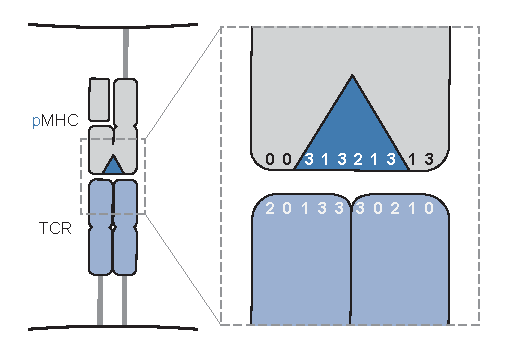
\includegraphics[width=0.48\textwidth]{Figures/intro/fig7_digitString.pdf}
    \caption[Digit-string representation of TCR:pMHC binding affinity]{%
    \textit{Digit-string representation of TCR:pMHC binding affinity}. %
    %
    The binding domains of the TCR, the peptide, and the MHC are modelled as a string of random numbers between 0 and 127 (only 0 to 3 shown here), with the affinity being proportional to the similarity between the TCR string and the compound peptide-MHC string. Adapted from~\cite{chao2005effects}.}
    \label{fig:intro_digitString}
\end{figure}

%%%%%%%%%%%%%%%%%%%%%%%%%%%%%%%%%%%%%%%%%%%%%%%%%
\subsection{Low-avidity T cells -- unsung heroes?}
\label{sec:intro_affinity_highVsLowAffinity}

Given their greater sensitivity to pMHC by definition, it is perhaps unsurprising that many groups have reported that T cells with higher foreign-pMHC reactivity predominantly respond to infection~\cite{busch1999t,king2012t,rosenthal2012low,mandl2013t,straub2023recruitment}. Indeed, in multi-clonal T cell population models where the probability of proliferation is higher for higher-avidity T cells, these cells outnumber their lower-avidity counterparts upon antigen-driven clonal expansion~\cite{de1994t,de1995towards,chao2004stochastic,chao2004modelling}. However, T cells that possess lower-affinity TCRs are known to also contribute to anti-microbial responses~\cite{martinez2015lower,martinez2016low,kolawole2020relationship}. Additionally, since autoreactive low-avidity T cells specific for self-pMHC predominantly escape negative selection and can cause autoimmunity as discussed in Section~\ref{sec:intro_autoimmunity_whyCentralAndPeripheral}, it follows that these T cells indeed possess the effector potential necessary to carry out immune responses~\cite{kolawole2020relationship}. Furthermore, emerging evidence suggests that, in both CD4\pos{} and CD8\pos{} T cells, those with lower-affinity TCRs may predominate in the case of chronic infection where the pathogen persists for extended periods of time within the host~\cite{gallegos2016control,tsitsiklis2020unusual,schober2020reverse}. However, given the difficulty in detecting these T cells (let alone assessing their function) within a polyclonal population using conventional experimental techniques, computational modelling can be a useful tool to investigate their contribution in controlling pathogen replication (Chapter~\ref{sec:AvC}). 

%%%%%%%%%%%%%%%%%%%%%%%%%%%%%%%%%%%%%%%%%%%%%%%%%
\subsection{Summary and highlights}
The peripheral pool of pathogen-specific T cells is composed of a TCR repertoire that may bind pathogen-derived pMHC across a wide range of affinities, with both low- and high-affinity T cells contributing to the response. However, to date there does not exist any perfect experimental technique that can simultaneously and comprehensively measure the affinity of all pathogen-specific TCR clonotypes across this large continuum. Specifically, T cells with low foreign-pMHC binding strength are often overlooked or go undetected, yet they may be important contributors to the anti-pathogen immune response. In Chapter~\ref{sec:AvC}, we used modelling to complement experimental techniques, with the goal of investigating the function of these T cells with lower pMHC binding strengths and how infection duration (i.e., chronic vs. rapidly cleared ``acute'' infections) might play a role.

%%%%%%%%%%%%%%%%%%%%%%%%%%%%%%%%%%%%%%%%%%%%%%%%%
%%%%%%%%%%%%%%%%%%%%%%%%%%%%%%%%%%%%%%%%%%%%%%%%%
\section{T cell escape}
\label{sec:intro_immuneEscape}

Over the course of an infection, what T cells will ``see'' is often not static. In fact, many pathogens have independently and remarkably evolved mechanisms to acclimate to their environment within the host and avoid detection by T cells in a process known as ``immune evasion''  or ``escape''. Pathogens do this in large part by manipulating the ability of TCRs to bind to their respective pathogen-derived pMHCs, thereby ``blinding'' T cells, in a sense, to their presence and preventing them from carrying out their anti-microbial responses. Thus, a tug-of-war exists between T cells and pathogens as the latter attempt to adapt to selective pressure exerted by the former. Notably, there are a large number of different strategies that pathogens may employ to evade detection or clearance by pathogen-specific T cell populations, and these will vary depending on the type of pathogen in question. While there is an entire branch within the field of microbiology dedicated to understanding the inner workings of these mechanisms, for the purposes of this thesis, I will provide only a broad overview of such strategies. 

%%%%%%%%%%%%%%%%%%%%%%%%%%%%%%%%%%%%%%%%%%%%%%%%%
\subsection{Mechanisms of T cell escape}
\label{sec:intro_immuneEscape_mechanisms}

The first common mechanism of immune escape worth discussing is the concept of ``dormancy'' or ``quiescence'', whereby bacterial pathogens such as \textit{Mycobacterium tuberculosis}, as well as some fungal pathogens, can enter states of non-reproduction and non-infectivity in order to ``hide'' from the host~\cite{rittershaus2013normalcy,shepherd2020t,brunet2018reactivation}. Though the underlying microbiological pathways are distinct, viruses can behave in a similar manner in a process known as viral ``latency'', where the viral genome resides within the host cell but suspends the production of new viral particles; this latent virus remains replication-competent in spite of its apparent dormancy, allowing it to become re-activated after potentially long times (even years)~\cite{speck2010viral,eshleman2011varicella,delannoy2019cat,zangger2022t}. In fact, the ability of human immunodeficiency virus (HIV) to be so elusive to anti-retroviral treatments is in no small part due to the presence of its latent reservoir of infected cells~\cite{chun1999latent,delannoy2019cat}. The dynamics of HIV infection have been modelled extensively (reviewed in~\cite{perelson2002modelling,rong2009modeling,hill2018mathematical}), and inclusion of these latent reservoirs in such models indeed demonstrated decreased likelihood for the potential of anti-retroviral therapies to achieve viral eradication in infected individuals.

Another mechanism adopted by a range of viral and intracellular bacterial pathogens to avoid detection by T cells is the induction of MHC class I (MHCI) downregulation~\cite{hewitt2003mhc,shepherd2020t,delannoy2019cat,antoniou2008pathogen}. Again, the molecular mechanisms employed to this effect are complex and heterogeneous (reviewed in~\cite{antoniou2008pathogen}), but generally speaking, they all serve to reduce recognition by CD8\pos{} T cells since these require interaction with pathogen-derived pMHC expression via their TCR to clear infected cells. \textit{Plasmodium} protozoa, the parasites responsible for malaria, also induce MHCI downregulation within infected Kupffer cells in the liver during the sporozoite stage of their life cycle~\cite{steers2005immune,gomes2016immune}. Additionally, these parasites have the advantage that, during their later merozoite stage, they infect anucleate red blood cells (RBCs) that do not express any MHC at their cell surface, thus impairing the ability of CD8\pos{} T cells to find and kill infected cells~\cite{gomes2016immune}. Furthermore, pathogens may take advantage of peripheral tolerance mechanisms whose aim is to suppress T cell responses~\cite{garib2015t} (see Section~\ref{sec:intro_autoimmunity_peripheralTolerance}). For example, they may alter APC function to induce the differentiation of pathogen-specific conventional T cells into immunosuppressive regulatory T cells such as Tr1 cells~\cite{belkaid2007regulatory,belkaid2009regulatory,garib2015t,boer2015regulatory}. In a similar vein, chronic stimulation of pathogen specific CD4\pos{} and CD8\pos{} T cells can drive functional exhaustion in these T cells. This exhausted phenotype is characterized by the loss of the ability of these T cells to carry out their anti-microbial functions, such as production and release of their signature pro-inflammatory cytokines or cytotoxic responses~\cite{zajac1998viral,wherry2011t,shepherd2020t}.

One T cell evasion strategy of particular relevance for this thesis is the concept of ``antigenic variation''. Briefly, antigenic variation entails genetic or epigenetic modifications that effectively alter what will be presented to T cells in the context of pMHC~\cite{deitsch2009common}. The former might involve mutations or recombination in the pathogen genome, while the latter refers instead to changes in their gene expression patterns. More complex microorganisms, such as bacteria, fungi, and protozoa, have evolved fairly intricate mechanisms of antigenic variation, including phase variation (switching individual genes between ``on'' and ``off' 'states) and mutually exclusive expression (alternating which genes from a large multi-copy gene family is actively transcribed), among others~\cite{van2004phase,deitsch2009common,florini2022shared}. Viruses, being much simpler microorganisms\footnote{Viruses are technically not microorganisms since they are not self-sustaining and not officially considered ``living'', though there is some debate around this~\cite{brown2016viruses}.} with much smaller (DNA or RNA) genomes that completely rely on the cellular machinery of the host cells they infect to sustain themselves and to reproduce, employ a different strategy. In fact, viruses (in particular RNA viruses such as HIV, but also DNA viruses to a lesser extent) have very high mutation rates originating in large part (though not exclusively) from genome replication errors~\cite{sanjuan2016mechanisms}. While most of these mutations are deleterious or even lethal for the virus~\cite{domingo2009fitness,wylie2011biophysical}, some might provide an adaptive advantage with one possible benefit being mutations in pMHC epitope regions of the viral genome, and thus T cell escape (Fig.~\ref{fig:intro_antigenicVariation}).

\begin{figure}
    \centering
    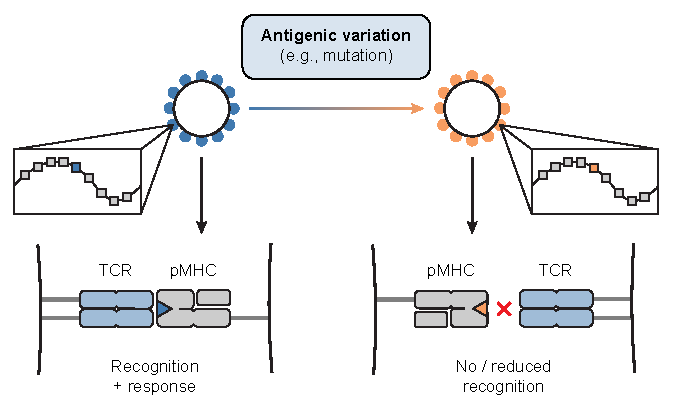
\includegraphics[width=0.64\textwidth]{Figures/intro/fig8_antigenicVariation.pdf}
    \caption[Antigenic variation as a mechanism of T cell escape]{\textit{Antigenic variation as a mechanism of T cell escape}. %
    %
    Some pathogens can undergo modifications (e.g., mutations as is typically the case for viruses, shown here) that alter what T cells will see via their TCR. Schematic insets depict a single amino acid substitution in the peptide sequence that becomes conjugated to the MHC molecule, thus altering the pMHC epitope. Antigenic variation can lead to an impaired capacity of the TCR to bind the altered pMHC, thus reducing or eliminating the ability of those T cells to respond to (and clear) the pathogen.}
    \label{fig:intro_antigenicVariation}
\end{figure}

\subsection{Within-host pathogen evolution -- lessons from RNA viruses}

RNA viruses that produce chronic infections within their host, such as HIV and hepatitis C virus (HCV), possess a remarkable capacity to evolve escape mutations in pMHC epitope regions of their genome, thus evading the anti-viral T cell response~\cite{weiner1995persistent,borrow1997antiviral}. This follows from the fact that, relative to all other microorganisms, RNA viruses have the highest replication error rate per nucleotide within their genome~\cite{peck2018complexities,sanjuan2016mechanisms}. Given the high propensity for these viruses to mutate with every replication cycle, together with short generation times and massive amounts of new virions being formed daily within an infected host (e.g., at least 10 billion per day in HIV as estimated from mathematical population models~\cite{perelson1996hiv,perelson2002modelling}), a viral population in biological systems is almost always comprised of a large collection of unique genomes; thus, the term ``quasispecies'' is used to describe such populations~\cite{andino2015viral,domingo2019viral,lauring2020within}.

\begin{figure}
    \centering
    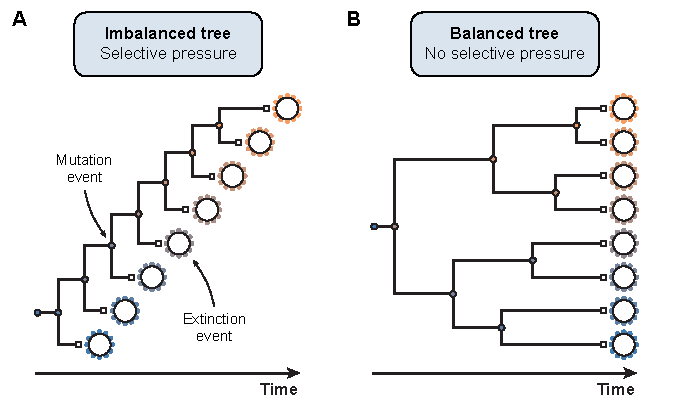
\includegraphics[width=0.64\textwidth]{Figures/intro/fig9_phylodynamics.pdf}
    \caption[Idealized representation of within-host phylodynamic tree topologies]{%
    \textit{Idealized representation of within-host phylodynamic tree topologies}. %
    %
    \secbfcolor{(A)}~Imbalanced (or ladder-like) tree architecture representing pathogen evolution under strong selective pressure. %
    %
    \secbfcolor{(B)}~Balanced (or star-like) tree architecture occurring in the absence of selective pressure on pathogen evolution. Adapted from~\cite{volz2013viral}.}
    \label{fig:intro_phylodynamics}
\end{figure}

Assessing the composition of viral quasispecies, and how they evolve over the course of an infection within a host, can be done using a combination of sequencing approaches and phylogenetic analyses~\cite{volz2013viral,lauring2020within}. ``Phylodynamic'' trees are often used to study the intersection between immunological and epidemiological processes that shape pathogen evolution within hosts (our interest for the purposes of this thesis) and also at the between-host/population scales~\cite{grenfell2004unifying,bons2018virus}; the latter will be revisited in Chapter~\ref{sec:conclusion} when discussing extensions and possible implications of our within-host studies. One example of the use of phylodynamic trees is that they can inform the evolutionary pressures present on the replicating pathogen, where imbalanced or ``ladder-like'' tree topologies reveal strong selection pressures influencing viral adaptation as compared to balanced trees (Fig~\ref{fig:intro_phylodynamics})~\cite{grenfell2004unifying,volz2013viral}. At the within-host level, these imbalanced trees have indeed revealed strong selection pressures shaping HIV and HCV evolution~\cite{grenfell2004unifying,raghwani2019high,lemey2006hiv}.

Influenza A virus (IAV) is another RNA virus with fairly high mutation rates~\cite{sanjuan2010viral}. While \textit{de novo} mutations do arise in infected hosts, when compared to HIV or HCV, IAV within-host evolution is limited by the fact that these viruses are usually cleared by the immune system within 5-7 days post-infection (as estimated from mathematical modelling of viral load kinetic data)~\cite{xue2018within,baccam2006kinetics}. However, in immunocompromised individuals where the infection may last much longer (weeks or months), extensive evolution and antigenic variation has been measured by longitudinal viral sampling of these hosts~\cite{rocha1991antigenic,mcminn1999antigenic,xue2017parallel}. Given the consequences that viral evolution within infected hosts may have on the epidemiology and spread of infectious diseases, studying how T cell-mediated immunity can shape this evolutionary process remains of utmost importance.

%%%%%%%%%%%%%%%%%%%%%%%%%%%%%%%%%%%%%%%%%%%%%%%%%
\subsection{Pathogen-immune co-evolution -- the role of T cell selective pressure}
\label{sec:intro_immuneEscape_RNAviruses}

As T cells play a fundamental role in orchestrating anti-microbial responses, it follows that they act as a major driver of within-host pathogen evolution by exerting strong selection pressures and shaping fitness landscapes that the pathogen must exploit in order to persist. While longitudinal viral sequencing studies can provide valuable information into how these pathogens are evolving over time within their host, simultaneously assessing the complimentary and dynamic role that T cells play in driving these changes using experimental techniques is challenging. Modelling efforts are thus needed to gain insight into how T cells and pathogens interact with one-another to generate outcomes observed from monitoring viral sequences. In 2004, Grenfell et al. described a simple conceptual model of how the balance between pathogen control and immune selection pressure may ultimately shape within-host pathogen evolution and the ensuing phylodynamic patterns observed for different viruses~\cite{grenfell2004unifying}. In their model, the number of advantageous mutations (and thus the propensity for the virus to adapt) results from a necessary combination of sufficient viral abundance and immune pressure favouring these mutations (Fig.~\ref{fig:intro_abundanceVsPressure}). This model formalism predicted a ``sweet spot'' where the product of these two quantities results in maximal potential for the virus to adapt under selection pressures exerted by the immune system.

\begin{figure}
    \centering
    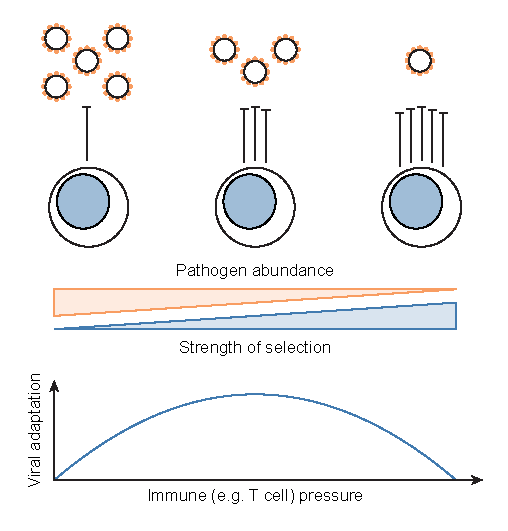
\includegraphics[width=0.48\textwidth]{Figures/intro/fig10_abundanceVsPressure.pdf}
    \caption[Conceptual model of viral adaptation as a function of immune pressure]{%
    \textit{Conceptual model of viral adaptation as a function of immune pressure}. %
    %
    Higher levels of immune-mediated control on viral replication decrease the abundance of the pathogen, but increase the strength of selection favouring viral evolution/adaptation to the host environment. The propensity for the virus to adapt is taken as a product of these two factors and peaks at intermediate immune pressures. Adapted from~\cite{grenfell2004unifying}.}
    \label{fig:intro_abundanceVsPressure}
\end{figure}

To study how HIV-T cell co-evolution and the production of new antigenic variants of the former leads to the eventual failure of T cells to control HIV replication and subsequently to the development of acquired immunodeficiency syndrome (AIDS), Nowak et al. developed a mathematical population model where unique variants of HIV, and their associated T cell responses, were explicitly distinguished from each other~\cite{nowak1991antigenic}. In their model, the probability that a new antigenic variant arises was taken to be proportional to HIV viral loads, which were negatively modulated by the responding T cell population. Based on their model formalism, they found that once the number of HIV variants exceeds a critical threshold, T cells specific for these antigens become overwhelmed and are no longer able to keep viral loads in check, leading to the onset of AIDS. In another model of HIV evolution and CTL escape, van Deutekom et al. showed that slow accumulation of escape mutations during the clinical latency phase of HIV infection leads to an eventual rise in the rate of escape at late stages of infection, which in turn drives higher viral loads and further amplifies the emergence of new mutants in a positive feedback loop until complete T cell escape is achieved~\cite{van2013rate}. While these models have certainly generated informative and useful insights, there is still a need to study more specific aspects of the the T cell response and how these in turn can modulate the ability of a pathogen to evolve within the host.

\subsection{Summary and highlights}

While T cells are indispensable for choreographing immune responses to pathogens, their anti-microbial functions exert a selective pressure that many pathogens have evolved to exploit, resulting in T cell escape and impaired control of pathogen replication. The potential consequences of this constant tug-of-war are all-too-familiar to us, having just lived through a pandemic where viral adaptation evidently led to the emergence of many pathogen variants that evaded pre-existing immunity and greatly complicated efforts to contain their spread. Thus, there is an imperative need for us to better understand how specific aspects of the T cell response can modulate the rates of immune escape. In Chapter~\ref{sec:VE}, we will study how TCR repertoire diversity might affect this balance between pathogen control and adaptation, by asking whether less diverse TCR repertoires might exacerbate the capacity of these pathogens mutating within their hosts to generate variants that escape T cell recognition.

\chapter{A neurophysiological basis for aperiodic EEG and the background spectral trend} \label{sec:natcomms}

One of the most promising theories of the EEG spectral trend is the synaptic timescales hypothesis (\autoref{sec:timescales}). According to this theory, the EEG spectral trend reflects asynchronous neural activity that is filtered by the kinetics of synaptic currents \cite{Bedard2006,Miller2009, Gao2017}. However, this theory remains underdeveloped in several ways. Firstly, the relative contributions of excitatory and inhibitory synaptic currents have not been defined. In early work, only a single synaptic timescale was considered \cite{Bedard2006,Miller2009}, whereas in later work, the ratio of excitatory to inhibitory currents was defined phenomenologically \cite{Gao2017}. Specifically, Gao et al. \cite{Gao2017} modelled the extracellular potential as a linear combination of multiple Poisson processes filtered by decaying exponentials of two different timescales, reflecting excitatory and inhibitory kinetics. It remains unclear whether the final ratio required to explain the spectral trend is consistent with realistic current amplitudes, synapse densities, firing rates, and the nonlinear membrane interactions of synaptic currents. 

Secondly, all past studies on this theory have simulated neural activity as a Poisson process, that is ``asynchronous'' neural activity, which is not thought to be capable of generating EEG signals. Thus, for the synaptic timescale hypothesis to be valid, these timescales must be filtering some sort of non-oscillatory neural activity that can generate detectable EEG signals. Whether such aperiodic EEG signals are possible has yet proven biophysically.

Thirdly, synaptic timescales have only been used to explain the $\beta=-2$ exponent observed in EEG spectra computed over many minutes of data. It remains to be determined whether this explanation is valid for EEG spectra computed over shorter time windows, and moreover whether this model captures the full broadband spectral properties of EEG, i.e., not just the parameterized slope within a specific frequency range. 

Finally, the interactions between the spectral trend and EEG oscillations has not been modelled under the synaptic timescale hypothesis. The findings from this theory inspired the FOOOF package to add a ``knee'' parameter, $k$, to their model for the spectral trend: $\alpha/(1+(f/k)^\beta)$. However, no studies found that synaptic timescales give rise to spectra of different scaling factors, $\beta$. Therefore, it is unclear whether this function, which allows for exponents different from $-2$ is truly the correct parameterization for accurate spectral detrending.

To address these shortcomings, I leveraged advances in the biophysical simulation of single-neuron dipoles (\autoref{sec:dipoles}) along with the recent availability of accurate, computationally efficient EEG forward models (\autoref{sec:head_models}). Using these computational tools, I developed new statistical and topological models of aperiodic EEG generation. To test predictions of the model, my advisor and I collaborated with anesthesiologists at the Montreal Neurological Institute who collected EEG recordings from patients undergoing infusions of drugs that pharmacologically alter the gating kinetics GABA receptors. Finally, I derived a physiologically-justified method for correcting the effects of synaptic timescales on EEG spectra and showed that applying this method to our collaborators' data produced more interpretable results than the traditional analysis of uncorrected spectra. The work presented in this chapter has been published and is a copy of the following paper:

\vspace{1em}
\hrule
\vspace{.5em}
\noindent
\hangindent=1cm
Brake, N., Duc, F., Rokos, A. \textit{et al.} A neurophysiological basis for aperiodic EEG and the background spectral trend. \textit{Nat Commun} \textbf{15}, 1514 (2024). https://doi.org/10.1038/s41467-024-45922-8
\vspace{.75em}
\hrule
\vspace{.65em}

\noindent
The article is licensed under a Creative Commons Attribution 4.0 International License, and is reproduced here with minor formatting changes. To view a copy of this licence, visit \url{http://creativecommons.org/licenses/by/4.0/}.


\newpage

\section{Abstract}
Electroencephalograms (EEGs) display a mixture of rhythmic and broadband fluctuations, the latter manifesting as an apparent $1/f$ spectral trend. While network oscillations are known to generate rhythmic EEG, the neural basis of broadband EEG remains unexplained. Here, we use biophysical modelling to show that aperiodic neural activity can generate detectable scalp potentials and shape broadband EEG features, but that these aperiodic signals do not significantly perturb brain rhythm quantification. Further model analysis demonstrated that rhythmic EEG signals are profoundly corrupted by shifts in synapse properties. To examine this scenario, we recorded EEGs of human subjects being administered propofol, a general anesthetic and GABA receptor agonist. Drug administration caused broadband EEG changes that quantitatively matched propofol’s known effects on GABA receptors. We used our model to correct for these confounding broadband changes, which revealed that delta power, uniquely, increased within seconds of individuals losing consciousness. Altogether, this work details how EEG signals are shaped by neurophysiological factors other than brain rhythms and elucidates how these signals can undermine traditional EEG interpretation.


\section{Introduction}
Electroencephalograms (EEGs) display a mixture of periodic and aperiodic fluctuations. Almost a century of research has established that periodic EEG signals are generated by synchronous neural oscillations\cite{Berger1929,Buzsaki2012,Nunez2006,steriade2005cellular}. In contrast, aperiodic EEG signals remain relatively poorly understood. Whereas periodic EEG signals produce peaks in power spectra, the aperiodic component manifests as the background spectral trend that decays with apparent $1/f^\beta$ behaviour\cite{He2014,Manning2009,Miller2009,Pritchard1992}. Differences in the spectral exponent, $\beta$, have been correlated with aging, cognitive performance, neurological disorders, anesthesia, and sleep\cite{Colombo2019,Lendner2020,Ouyang2020,Roche2019,Voytek2015,Donoghue2020}. In addition to being a useful biomarker, it has been proposed that the EEG spectral trend may change independently of neural oscillations and that spectral detrending is necessary to accurately quantify differences in brain rhythms\cite{Donoghue2020}. Deciphering the neurophysiological basis of aperiodic EEG is thus necessary for correctly interpreting EEG biomarkers and for improving algorithms that quantify brain rhythms.

There exist two main hypotheses for how the EEG spectral trend is generated by the brain. The synaptic timescale hypothesis predicts that the EEG spectral trend is a natural consequence of exponentially decaying synaptic currents, and that consequently asynchronous network activity will produce a spectrum with a $1/(1+\tau^2f^2)$ or “Lorentzian” trend\cite{Bedard2006,Gao2017,Miller2009}. The second hypothesis is based on the theory of self-organized criticality which posits that the propagation of action potentials throughout neural networks produces so-called “avalanches” of activity with magnitudes following a $1/f$ distribution\cite{Bak1987,Beggs2003,Priesemann2014}. It has been hypothesized that such avalanche dynamics in turn generate a $1/f$ trend in EEG\cite{Chaudhuri2018,He2014,Lombardi2017}. These theories are different in two important respects. Firstly, the avalanche hypothesis implies that the trend in EEG spectra is informative about the dynamics of the brain, while the synaptic timescales hypothesis is agnostic. Secondly, the two theories suggest different shapes for the spectral trend and therefore propose distinct methods for detrending EEG spectra\cite{Donoghue2020}.  

Despite these hypotheses, the concept of aperiodic EEG itself remains controversial. Some argue that the apparent trend in EEG spectra is an epiphenomenon caused by slower brain rhythms recruiting larger populations of neurons\cite{Buzsaki2004, Buzsaki2023}. According to this viewpoint, the EEG spectrum does not require detrending and the spectral exponent is a conflated measure of various changes in brain rhythms. 

Three questions therefore remain open: (1) can EEG signals reflect arrhythmic neural activity? (2) if so, how do these signals shape EEG spectra? (3) do EEG spectra need to be detrended, and if so, what is the most physiologically meaningful method of detrending? To investigate these questions, we combined numerical forward modelling of scalp potentials with biophysical calculations of single-neuron dipoles \cite{Hagen2016,Huang2016, Næss2021}. With this approach, we simulated biophysically realistic EEG signals generated by networks exhibiting a range of dynamics. These simulations revealed several mechanisms, besides brain rhythms, that affect EEG signals and together shape the spectral trend. To test model predictions, we recorded EEG of humans receiving an infusion of the drug propofol, a general anesthetic that targets GABA receptors and slows the decay time of inhibitory synaptic currents\cite{Franks2008,Kitamura2003,Orser1994, Whittington1996}. These experiments identified specific EEG changes during propofol administration that were expected to contaminate brain rhythm estimates. Using our modelling insights, we corrected for these sources of contamination and reevaluated known EEG signatures of losing consciousness. Overall, this study develops a biophysically grounded theory describing the neural basis of aperiodic scalp potentials and provides practical conclusions for the spectral analysis of EEG data.

\section{Results}
\subsection{EEG cannot reflect asynchronous neural activity}
To understand the neurophysiology that underlies the EEG spectral trend, we began by investigating the properties of EEG generation at the single-neuron level. These properties are informative because they shape the ensemble EEG regardless of coherence or neural synchrony (See Definitions and Theoretical Framework in Methods). To examine these properties, we performed simulations of biophysically and morphologically detailed neuron models (\autoref{fig:figure2.1}a). To start, we did not assume any dynamics of presynaptic neurons and therefore modelled synaptic input with independent Poisson spike trains (\autoref{fig:figure2.1}a), an assumption that we relax later. From these currents, a single-neuron dipole was computed\cite{Næss2021} (\autoref{fig:figure2.1}b). The neuron was placed at a random location in the cortex and the single-neuron EEG signal was calculated using the New York head model\cite{Huang2016} (\autoref{fig:figure2.1}c). This entire procedure was repeated many times with various representative neuron morphologies (Table S1) and with the neurons placed at various locations in the cortex. The average spectrum, which we will refer to as a unitary spectrum, is the expected EEG spectrum generated by a single average cortical neuron (\autoref{fig:figure2.1}d). 


\begin{figure}[t!]
    \centering
    \centerline{\includegraphics[width=177mm]{Figures/chapter2/figure1.pdf}}

    \centerline{
    \begin{minipage}[c]{177mm}
    \caption{\captiontitle{EEG cannot reflect asynchronous neural activity.} \textbf{a} Example morphology of a layer 2/3 pyramidal neuron. Inputs at AMPAR (red) and GABAR (blue) synapses were simulated with Poissonian spike trains, shown in raster plot. Only 1,000 synapses shown for clarity. Neuron morphology adapted from Budd, J. M. L. \textit{et al.} Neocortical axon arbors trade-off material and conduction delay conservation. PLoS Comput. Biol. 6, e1000711 (2010). \textbf{b} The $x$, $y$, and $z$ components of the single-neuron dipole vector, calculated from (\textbf{a}). \textbf{c} Left: single-neuron EEG signals were simulated at the marked electrode location, with the neuron located at various source locations, e.g. location A and B. Right: the location-averaged EEG spectrum (black) computed by averaging over the source locations shown in black dots on the brain template. Loc.=location; Avg.=average. \textbf{d} Location-averaged spectrum generated from 1000 simulations of 11 representative neuron morphologies (Table S1). The spectrum was fit by Eq.~\ref{eq:linear_model} and the two Lorentzian components are shown in dashed red lines. \textbf{e} The unitary spectrum was calculated while varying the deactivation kinetics of GABARs ($\tau_I$) and the parameter $\tau_1$ was estimated. Red line has a slope of 1. \textbf{f} Same as (\textbf{e}), but showing $\tau_2$ as a function of the deactivation kinetics of AMPARs ($\tau_E$). \textbf{g} Sampling distributions for model parameters. $\lambda_E$, $\tau_E$, and $g_E$ represent the average input rate, the deactivation time constant, and maximal conductance for AMPAR synapses. $\lambda_I$, $\tau_I$, and $g_I$ represent the same parameters for GABAR synapses. $E_L$ and $g_L$ represent the reversal potential and conductance of the passive membrane leak current. \textbf{h} Distribution of single-neuron EEG power (location-averaged as in \textbf{c}) based on 20000 simulations with parameters sampled from the distributions shown in g and morphologies sampled as described in Table S1. \textbf{i} Black: Median EEG spectrum across 14 subjects, with error bands indicating minimum and maximum spectral density. Grey: the predicted EEG spectrum of 16 billion uncorrelated neurons receiving Poissonian synaptic input (grey), with parameter values sampled from the distributions in (\textbf{a}). Error bands reflect 5 to 95\% quantile range.} 
    \label{fig:figure2.1}
    \end{minipage}
    }
\end{figure}

The unitary spectrum exhibited two important features. First, even with random synaptic input, the unitary spectrum displayed a trend. This trend could be described as the sum of two Lorentzian functions
\begin{equation} \label{eq:linear_model}
    S(f) = \frac{A_1}{1+(2\pi \tau_1 f)^2} + \frac{A_2}{1+(2\pi \tau_2 f)^2}
\end{equation}
as predicted by simple linear models of EEG generation \cite{Gao2017,Miller2009} (\autoref{fig:figure2.1}d). The slower ($\tau_1$) and faster ($\tau_2$) timescales were governed by the deactivation kinetics of GABA receptors (GABARs) and AMPA receptors (AMPARs), respectively (\autoref{fig:figure2.1}e, f). These simulations validate previous predictions that the relative contribution of excitatory and inhibitory currents to the EEG signal fundamentally affects the spectral trend \cite{Gao2017}.

Second, the unitary spectrum reflects the amplitude with which an average neuron contributes to the EEG signal. To investigate this idea in more detail, we examined the effect of varying all the model parameters within physiologically reasonable ranges (\autoref{fig:figure2.1}g). Measuring the average power of the resulting single-neuron EEGs revealed a range of possible amplitudes for the contribution of individual neurons to the EEG signal (\autoref{fig:figure2.1}h). These simulations show that no physiologically plausible parameters could allow  \cite{Gao2017} billion uncorrelated neurons to generate detectable EEG signals (\autoref{fig:figure2.1}i). More importantly, these calculations quantify how far off a completely asynchronous cortex is from generating detectable EEG signals. These calculations account for the EEG strength contributed by synaptic current amplitudes, neuron geometry, average firing rate of neurons, the number of neurons, the conductivity of various tissues, and the geometry of the cortex. Therefore, this result indicates that neural dynamics are responsible for the approximate four orders of magnitude difference between the simulated asynchronous spectrum and real EEG recordings.

\subsection{Detectable EEG requires only weak, locally synchronized dipoles}
If the amplitude of EEG signals precludes asynchronous activity from shaping EEG spectra, what types of arrhythmic activity could influence EEG signals? To begin addressing this question, we first quantified in general how much dipole correlation is required to generate detectable EEG signals. To do so, we imposed a simplified spatial organization on a cortical template whereby neighbouring neurons produced correlated dipoles. Specifically, the dipoles of neurons separated by d \unit{\milli\meter} were correlated with a coefficient of $\rho(d)=\rho_{max}\exp{(-d^2/\sigma^2)}$, where $\rho_{max}$ is the maximal dipole correlation and $\sigma^2$ is the spatial scale over which correlations decline (\autoref{fig:figure2.2}a). Based on this correlation scheme, the geometry of the cortex, average densities of neurons, and the single-neuron EEG amplitudes from the previous section, we estimated the power of the ensemble EEG signal that would be produced with different values of $\rho_{max}$ and $\sigma^2$ (see Methods). To capture the EEG spectral trend, we estimated that broadband EEG signals need to have a total power of between 50 and 200 \unit{\micro\volt\squared} (\autoref{fig:figure2.2}b). Thus for neural activity to generate detectable EEG signals, this activity needs to be capable of driving single-neuron dipoles that are correlated up to a value ($\rho_{max}$) of 0.06 to 0.12 (\autoref{fig:figure2.1}c), assuming a liberal range for $\sigma^2$ of 5-13 \unit{\milli\meter} (\autoref{fig:figure2.1}c; see Methods). While the existence of EEG rhythms prove that neural oscillations can generate the requisite dipole synchrony, it remains to be determined if and how such a degree of dipole coherence may be achieved by arrhythmic neural activity. 

\begin{figure}
  \begin{minipage}[c]{77mm}
    \includegraphics[width=\textwidth]{Figures/chapter2/figure2.pdf}
  \end{minipage}\hfill
  \begin{minipage}[c]{77mm}
    \caption{ \captiontitle{Detectable EEG signals require only weak, locally synchronized dipoles.}
	\textbf{a} Schematic displaying the coupling kernel used to correlate single-neuron dipoles. The kernel is a Gaussian function with peak of $\rho_{max}$ and variance $\sigma^2$.
	\textbf{b} Median EEG spectrum across 14 human subjects (grey; same error bands as \autoref{fig:figure2.1}i), and simulated unitary spectrum (black; same as \autoref{fig:figure2.1}d) scaled by arbitrary amounts to determine a lower and upper bound of the spectral trend amplitude. 
	\textbf{c} Heatmap of the total simulated EEG power produced by 16 billion neurons with dipoles coupled with the kernel in (\textbf{a}), and parameterized with various values of $\rho_{max}$ and $\sigma^2$. The black lines are level curves representing the lower and upper bounds for the spectral trend magnitude obtained in (\textbf{b}).
    } \label{fig:figure2.2}
  \end{minipage}
\end{figure}

\subsection{Synapse topology is sufficient for dipole correlations}
To investigate the ability of neural activity to generate coherent dipoles, we simulated dyads of neurons and investigated the level of correlation achievable between the two single-neuron dipoles. In our simulations, we noticed that if a single synapse was activated, the orientation of the resulting dipole could be accurately predicted by the orientation of the synapse relative to the soma (\autoref{fig:figure2.3}a, b). This result held across all neuron morphologies investigated (\autoref{fig:figureS2.1}). From this observation, we devised a minimal model of dipole coherence. To generate synaptic input, we projected the synapses of two neurons onto a sphere and correlated the inputs of synapses with close angular distances (\autoref{fig:figure2.3}c). By changing the maximal correlation between synapses, dipole correlation between neurons of various morphologies could be tuned continuously between 0 and ${\sim}0.3$ (\autoref{fig:figure2.3}d, e). Shuffling the location of the synapses abolished any dipole correlation (\autoref{fig:figure2.3}d). These results demonstrate that to generate detectable EEG signals, it is necessary and sufficient for synaptic input to exhibit temporal and spatial correlation. These conditions do not by themselves preclude any specific type of neural dynamics. Indeed this minimal model relied on independently sampled spikes at every time point and thus generated EEG signals with no temporal autocorrelation and a spectrum with the same shape as the asynchronous unitary spectrum (\autoref{fig:figure2.3}f). Therefore, the plausibility of aperiodic EEG signals depends solely on the ability for a network of neurons to generate arrhythmic activity with the requisite levels of spatiotemporal correlation. 

\begin{figure}[t!]
    \centering
    \includegraphics[width=125mm]{Figures/chapter2/figure3.pdf}
    \caption{\captiontitle{A minimal model of dipole correlation captures broadband EEG amplitude but not low frequency power.}
	\textbf{a} A single synapse was activated at the location specified by the blue arrow, generating a response in the single-neuron dipole, Q. The dipole vector at the peak of the response is oriented towards the synapse location, defined in spherical coordinates with the soma as the origin. Neuron morphology adapted from Budd, J. M. L. \textit{et al.} Neocortical axon arbors trade-off material and conduction delay conservation. PLoS Comput. Biol. 6, e1000711 (2010).
	\textbf{b} The simulation in (\textbf{a}) was repeated 600 times with different neuron morphologies and synapse locations. Plotting the dipole orientation at the peak of the response against the location of the stimulated synapse shows a strong, linear relationship. Some points not plotted for clarity. Dot size is proportional to peak dipole amplitude. rel.=relative. 
	\textbf{c} Schematic showing the minimal model for dipole correlation. Synapses on each postsynaptic neuron in the dyad were projected onto a sphere. A correlation matrix among all synapses was then defined such that synapses separated by an angle $\theta_{ij}$ on the sphere were correlated by $R_{max}\exp{(-\theta_{Ij})}$. The left neuron’s morphology is adapted from Budd, J. M. L. \textit{et al.} Neocortical axon arbors trade-off material and conduction delay conservation. PLoS Comput. Biol. 6, e1000711 (2010). The illustration of the right neuron is adapted, with permission from SNCSC, from Mainen, Z. F. \& Sejnowski, T. J. Influence of dendritic structure on firing pattern in model neocortical neurons. Nature 382, 363–366 (1996), Springer Nature.
	\textbf{d} Example of single-neuron EEG signals of the two neurons shown in (\textbf{c}).
	\textbf{e} Correlation between two single-neuron dipoles as a function of $R_{max}$. Vertical lines represent 95\% confidence intervals of the mean ($n=11$ different morphology pairs). When synapse locations are shuffled, dipoles are no longer correlated (grey).
	\textbf{f} The unitary spectrum of neurons receiving input calculated with the minimal model (black), scaled to compare the shape of the spectrum with median EEG spectrum of 14 subjects (grey line; same as \autoref{fig:figure2.1}i).} 
    \label{fig:figure2.3}
\end{figure}


\subsection{Subcritical networks can generate aperiodic EEG signals}
We next investigated network models that could generate detectable, aperiodic EEG signals. To determine whether network activity could produce coherent dipoles, we utilized the results from the previous section (\autoref{fig:figure2.3}). After simulating a presynaptic neuron population, we used the UMAP algorithm\cite{McInnes2018} to embed the population onto a sphere in such a way that minimized the distance between presynaptic neurons with correlated spiking activity (\autoref{fig:figure2.4}a). These presynaptic neurons were then projected onto the dendrites of the postsynaptic dyad (\autoref{fig:figure2.4}a). By construction, synapses with higher correlations should have smaller angular distances, thus optimizing for dipole coherence. Effectively, this procedure tests whether it is geometrically possible for a network to generate sufficiently coherent synaptic input for EEG generation. 


\begin{figure}[t!]
    \centering
    \centerline{\includegraphics[width=180mm]{Figures/chapter2/figure4.pdf}}

    \centerline{
    \begin{minipage}[c]{180mm}
    \caption{\captiontitle{Subcritical network dynamics can explain the amplitude and low frequency power of broadband EEG.}
	\textbf{a}~Illustration of the algorithm for optimizing dipole coherence. Nrn. = neuron. The left neuron morphology is adapted from Budd, J. M. L. \textit{et al.} Neocortical axon arbors trade-off material and conduction delay conservation. PLoS Comput. Biol. 6, e1000711 (2010). The illustration of the right neuron is adapted, with permission from SNCSC, from Mainen, Z. F. \& Sejnowski, T. J. Influence of dendritic structure on firing pattern in model neocortical neurons. Nature 382, 363–366 (1996), Springer Nature.
	\textbf{b} Illustration of the rules used to produce spatiotemporal synchrony in a presynaptic network. Rule \#1: network topology is enforced by making the probability of pairwise connections, $P(C_{ij})$, decrease exponentially with distance, $d_{ij}$. Rule \#2: the probability of a neuron firing, $P_{t+1}$, depends on a baseline firing rate of $\lambda=\lambda_0(1-m)$ plus the average activity of its neighbours scaled by $m$. $\lambda_0$ is a predefined average firing rate; $m$ is the branching number of the network. corr.=correlation.
	\textbf{c} Examples of single-neuron EEG signals of two neurons receiving input from the network model with a branching number $m=0.98$, when synapse locations have been optimized as described in (\textbf{a}). Bottom: a raster plot of synaptic input for the two neurons. 
	\textbf{d} Correlation between two single-neuron dipoles as a function of the branching number, m, of the presynaptic network. Dipole correlation increases with $m$ (coloured dots), but not when synapse locations are shuffled (grey).  Median (dots) and 5 to 95\% quantile range (vertical lines) across $n=10000$ simulated dyads with randomly sampled morphologies (Table S1) and randomly sampled biophysical parameter values (as in \autoref{fig:figure2.1}g).
	\textbf{e} Dipole correlation can be tuned by placing synapses suboptimally (see Methods). Cubic interpolation between simulated optimality indices is shown with the solid line. Median (dots) and 5 to 95\% quantile range (vertical lines) across n=500 simulations.
	\textbf{f} Unitary spectra calculated for different branching numbers. Error bands reflect 95\% confidence interval of the mean.
	\textbf{g} The unitary spectra from (\textbf{f}) scaled based on a synapse optimality index of 0.25 (colours same as in \textbf{f}). The value of $\rho_{max}$ was determined from (\textbf{e}) and the final scaling factor was determined as in \autoref{fig:figure2.2}. Grey: median EEG spectrum of 14 subjects (same as \autoref{fig:figure2.1}i).} 
    \label{fig:figure2.4}
    \end{minipage}
    }
\end{figure}


To understand the mechanisms of aperiodic EEG generation, we attempted to construct the simplest network that could generate dipole coherence. Our previous results demonstrate that randomly connected networks cannot generate coherent dipoles, because they cannot produce spatially correlated activity. We therefore continued on to use the simplest neural network that exhibits spatial topology, namely, a spatial network. To construct the network, each neuron was embedded in a plane and connected preferentially to nearby neurons (\autoref{fig:figure2.4}b). For simplicity, we modelled individual neurons as binary nodes, i.e., each neuron was either spiking or quiescent. Spikes propagated along network connections, causing subsequent neurons to fire with some probability (\autoref{fig:figure2.4}b). This simple model falls within the category of a branching network, because the dynamics are governed by a single parameter called the branching number, denoted by m, which reflects the average number of spikes successfully elicited across the network when a single neuron fires. 

Our simulations revealed that the maximal achievable dipole correlation increased with the network’s branching number (\autoref{fig:figure2.4}c, d). A purely asynchronous network ($m=0$) was unsurprisingly incapable of generating correlations among single-neuron dipoles (\autoref{fig:figure2.4}d). On the other hand, a slightly subcritical network ($m=0.98$) was capable of generating dipoles that were correlated by $0.18 \pm 0.001$ for an average pair of postsynaptic neurons (mean $\pm$ SE, $n=10000$; morphologies sampled as described in Table S1; biophysical parameters sampled as in \autoref{fig:figure2.1}g). This branching number is significant because previous work has found that networks with a branching number of m=0.98\ closely reproduced the in vivo dynamics of cortical spiking across many different species \cite{Suryadi2022, Wilting2019}, making this a physiologically plausible parameter value. Placing synapses suboptimality led to proportionally lower dipole correlation, revealing that subcritical dynamics can still drive coherent dipoles with suboptimal synapse placement (\autoref{fig:figure2.4}e). Based on the amplitude of the computed unitary spectrum (\autoref{fig:figure2.4}f), we estimated that subcritical network activity can produce realistic EEG amplitudes with synapse optimality as low as ${\sim}25$\% (\autoref{fig:figure2.4}g; see Methods). As a reference, an optimality index of 50\% means that strongly correlated synapses will on average lie on the same hemisphere of their respective neurons, a geometry reminiscent of the apical-basal compartmentalization of cortical pyramidal neurons. 

Notably, stronger dipole correlations coincided with longer temporal autocorrelations in network activity (\autoref{fig:figure2.4}f), a phenomenon directly resulting from the causality of spike propagation (\autoref{fig:figure2.4}b). This means that EEG signals produced by propagating cortical spikes must have higher power at low frequencies if the signals are to be of detectable amplitudes. This result illustrates a fundamental constraint that may in part explain the 1/f scaling of EEG spectra at lower frequencies (\autoref{fig:figure2.4}g). More broadly, these results demonstrate a biophysically feasible mechanisms that allows arrhythmic neural activity to generate EEG signals, and to consequently influence the broadband features of EEG spectra.

\subsection{Narrowband EEG changes could result from arrhythmic activity}
The above calculations show that arrhythmic neural activity can in theory generate broadband EEG signals, meaning that narrowband EEG power need not reflect brain rhythms. We therefore asked whether EEG signals that are produced by arrhythmic activity can confound traditional EEG interpretation, namely, that changes in bandpower reflect differences in neural oscillations. To address this question, we considered a scenario where the EEG signal is generated by two subpopulations of neurons: a population exhibiting synchronous oscillations, and a second population exhibiting subcritical dynamics ($m=0.98$). If these population are completely independent of one another, their EEG contributions will by definition add together linearly. To investigate further, we simulated the scenario in which the two populations’ postsynaptic signals are intermixed (\autoref{fig:figure2.5}a). One interpretation of this setup could be a cortical neuron that is receiving oscillatory input from, say, the thalamus, while also receiving subcritical input from the local cortical circuitry. Compared to neurons receiving entirely oscillatory input or entirely subcritical input, the neuron receiving mixed input produced a unitary EEG spectrum that exhibited a mixed phenotype (\autoref{fig:figure2.5}b). Increasing the strength of the oscillatory and/or aperiodic input altered the amplitude of the spectral peak and/or spectral trend (\autoref{fig:figure2.5}c-e). However, changes to the spectral trend did not multiplicatively scale the oscillatory peak amplitude. As a result, quantifying the amplitude of oscillatory peaks relative to the spectral trend produced incorrect interpretations (\autoref{fig:figure2.5}f-h): dividing the peak amplitude by the background trend erroneously suggested that the neural rhythm decreased when aperiodic activity became stronger (\autoref{fig:figure2.5}d, g), and severely underestimated the neural rhythm increase when aperiodic activity increased concomitantly (\autoref{fig:figure2.5}e, h). We therefore concluded that if a spectral peak is clearly discernible, then arrhythmic neural activity has a minimal confounding influence and detrending is unnecessary. Importantly, however, if no spectral peak is obvious, then there is no guarantee that changes in power result from differences in neural oscillations.

\begin{figure}[t!]
    \centering
    \centerline{\includegraphics[width=176mm]{Figures/chapter2/figure5.pdf}}

    \centerline{
    \begin{minipage}[c]{176mm}
\caption{\captiontitle{Measuring oscillatory peak power relative to spectral trend may produce misleading results.}
	\textbf{a} Illustration of mixed input model. Half of the neuron’s synapses received oscillatory rhythmic input (blue) and the other half received input from a subcritical network (red). The strengths of oscillatory and subcritical dynamics were adjusted by tuning two parameters, $\alpha_R$ and $\alpha_A$, respectively, which determined the degree to which synaptic inputs differed from homogenous Poisson processes. See Methods for details. Neuron illustration created with BioRender.com.
	\textbf{b} Unitary spectrum for neurons receiving Poisson input (grey), compared with the unitary spectra for neurons receiving input entirely from the oscillatory population (left; black), entirely from the subcritical population (middle; black), or mixed input as in a (right; black): $\alpha_R=\alpha_A=0.1$.
	\textbf{c} Oscillatory input was strengthened by increasing $\alpha_R$ from 0.1 (black) to 0.5 (blue), with $\alpha_A$ fixed at 0.1. The spectra were fit using a FOOOF-like algorithm\cite{Donoghue2020}, except that here the aperiodic component was modelled with Eq.~\ref{eq:linear_model} (solid grey line).
	\textbf{d} Aperiodic input was strengthened by increasing $\alpha_A$ from 0.1 (black) to 0.5 (red), with $\alpha_R$ fixed at 0.1.
	\textbf{e} Both oscillatory and aperiodic inputs were strengthened by increasing both $\alpha_R$ and $\alpha_A$ from 0.1 (black) to 0.5 (magenta).
	\textbf{f} Detrended spectrum of neurons receiving mixed input before (black) and after (blue) oscillation strength increased. The unitary spectra in (\textbf{c}) were divided by the solid grey line. 
	\textbf{g} Detrended power before (black) and after (red) aperiodic strength increases. Notice that the detrended power at \qty{2}{\hertz} decreases, despite the strength of oscillations remaining the same.
        \textbf{h} Detrended power before (black) and after (magenta) both oscillation and aperiodic strength increases. Notice that the detrended power at \qty{2}{\hertz} does not increase as much as in (\textbf{f}), despite the oscillation increasing in strength by the same amount.} 
    \label{fig:figure2.5}
    \end{minipage}
    }
  
    
\end{figure}


\subsection{Spectral slope is an inconsistent measure of EI balance}
The above results focused on the role of neural dynamics in shaping the EEG spectrum. However, Figs. 1d-f show that the kinetics of postsynaptic responses also impact the broadband properties of EEG spectra. To further investigate this mechanism shaping EEG spectra, we performed a full sensitivity analysis of the spectral slope with respect to the biophysical parameters in the single-neuron models. The unitary EEG spectrum was simulated with many different parameter values (\autoref{fig:figure2.6}a) and the overall slope of the spectrum was calculated \cite{Donoghue2020} between 1 and 40 \unit{\hertz} (\autoref{fig:figure2.6}b). These simulations revealed that the spectral slope was consistently affected by four parameters: $\tau_I$, $g_E$, $g_I$, and $E_L$ (\autoref{fig:figure2.6}c). These results can be explained through Eq.~\ref{eq:linear_model}. The parameter $\tau_I$ directly determines the slow timescale, $\tau_1$, of the unitary spectrum (\autoref{fig:figure2.1}d), whereas synaptic conductances, $g_E$ and $g_I$, directly govern the contributions of inhibitory and excitatory synaptic currents, respectively. The reversal potential, $E_L$, of the leak current alters the spectral slope because when $E_L$ is more depolarized, GABA\textsubscript{A} receptors experience a higher driving force, thus amplifying the contributions of inhibitory currents. 


\begin{figure}
  \begin{minipage}[c]{90mm}
    \includegraphics[width=\textwidth]{Figures/chapter2/figure6.pdf}
  \end{minipage}\hfill
  \begin{minipage}[c]{70mm}
    \caption{
       \captiontitle{Sensitivity of spectral slope to biophysical parameters governing postsynaptic responses.}
	\textbf{a} Sampling distributions for model parameters, the same as the ones used in \autoref{fig:figure2.1}g.
	\textbf{b} Example single-neuron EEG spectrum, fitted with the equation ${10}^\alpha/f^\beta$ between 1 and \qty{40}{\hertz}.
	\textbf{c} Sensitivity of the spectral slope, $\beta$, to model parameters, with first and second order interactions, calculated from 20000 simulated spectra.
	\textbf{d} Simulated spectra were averaged depending on the ratio between $\lambda_E$ and $\lambda_I$. Lower E:I ratios correspond to more inhibition.
	\textbf{e} The spectral slope is plotted against the E:I ratio for each simulation. Left: simulation where the leak conductance was low ($g_L<0.1$ \unit{\milli\siemens\per\centi\meter\squared}; $n=7366$ simulations). Right: simulation where the leak conductance was high ($g_L>1$ \unit{\milli\siemens\per\centi\meter\squared}; $n=5184$ simulations).
    } \label{fig:figure2.6}
  \end{minipage}
\end{figure}

Surprisingly, the analysis of the spectral slope revealed a strong interaction between $g_L$ and both $\lambda_E$ and $\lambda_I$ (\autoref{fig:figure2.6}c). When the leak conductance was low ($g_L<0.1$ \unit{\milli\siemens\per\centi\meter\squared}), the spectral slope was found to be negatively correlated with the $\lambda_E$:$\lambda_I$ ratio (\autoref{fig:figure2.6}d, e; \autoref{fig:figureS2.2}b), which contradicts the predictions of linear models of EEG generation \cite{Gao2017}. The reason is that when the leak conductance was low, higher E:I ratios drove the average membrane potential close to the reversal potentials of GABA receptors (\autoref{fig:figureS2.2}a). This caused neurons with low $g_L$ to experience vanishing GABAR driving forces and amplified AMPAR driving forces at high E:I values, consequently and counterintuitively making the spectral slope anticorrelated with the E:I ratio (\autoref{fig:figure2.6}e). However, when the leak conductance was high ($g_L>1$ \unit{\milli\siemens\per\centi\meter\squared}), the membrane potential fluctuated less and stayed within a relatively linear regime (\autoref{fig:figureS2.2}a). Consequently the spectral slope was positively correlated with E:I ratio (\autoref{fig:figure2.6}e) as predicted by linear models of EEG generation \cite{Gao2017}. A similar albeit weaker effect was observed in the relationship between the spectral slope and the $g_E$:$g_I$ ratio (\autoref{fig:figureS2.2}c). Generally, we conclude that the overall spectral trend is significantly affected by biophysical parameters that alter postsynaptic responses, but changes in the slope value do not alone inform what parameters are changing.

\subsection{Changes to synaptic responses confound brain rhythm quantification}
Differences in postsynaptic responses alter EEG spectra in a fundamentally different way to arrhythmic neural activity. Postsynaptic kinetics effectively interact as a convolution with synaptic input and should therefore interact with oscillatory peaks in a multiplicative manner. Moreover, postsynaptic mechanisms should affect power generated by all types of neural dynamics equally. To test this, we systematically altered the biophysical parameters that govern postsynaptic currents and analyzed the unitary spectra generated by various types of synaptic inputs, including white noise (\autoref{fig:figureS2.3}), subcritical dynamics (\autoref{fig:figure2.7}a), as well as three types of dynamics that exhibit spectral peaks: a recently proposed recurrent Ising model that exhibits co-existence of oscillations and avalanches\cite{Lombardi2023} (\autoref{fig:figureS2.3}), an underdamped second-order system driven by white noise (\autoref{fig:figureS2.3}), and finally a simple sinusoidal rhythm (\autoref{fig:figure2.7}b). We investigated the effects of neurophysiological parameters that affect the spectral slope, as identified by our sensitivity analysis (\autoref{fig:figure2.6}c): GABAR kinetics ($\tau_I$), the leak current reversal potential ($E_L$), and the conductances of excitatory ($g_E$) and inhibitory ($g_I$) synapses. Changing these parameters altered the unitary spectra in distinct manners, but importantly had identical effects across the different types of the input dynamics (\autoref{fig:figure2.7}a, b; \autoref{fig:figureS2.3}). 


\begin{figure}
  \begin{minipage}[c]{90mm}
    \includegraphics[width=\textwidth]{Figures/chapter2/figure7.pdf}
  \end{minipage}\hfill
  \begin{minipage}[c]{70mm}
    \vspace*{0.25cm}
    \caption{
       \captiontitle{Changes in postsynaptic mechanisms confound brain rhythm quantification.}
	\textbf{a} Unitary spectra for neurons receiving entirely subcritical input ($m=0.98$,$\alpha_A=0.1$; see \autoref{fig:figure2.5}a), before and after four parameter changes: subplot corresponding to ($\uparrow\tau_I$) shows the unitary spectrum when $\tau_I$  was increased from \qty{10}{\milli\second} (pink) to \qty{30}{\milli\second} (red); $(\uparrow E_L$) shows unitary spectrum when $E_L$ was increased from \qty{-60}{\milli\volt} (pink) to \qty{-45}{\milli\volt} (red); ($\uparrow g_E$) shows unitary spectrum when $g_E$ was increased from \qty{0.7}{\nano\siemens} (pink) to \qty{1.4}{\nano\siemens} (red); and ($\uparrow g_I$) shows unitary spectrum when $g_I$ was increased from\qty{0.7}{\nano\siemens} (pink) to \qty{1.4}{\nano\siemens} (red). Note the changes in the unitary spectra despite there being no changes in synaptic input dynamics.
	\textbf{b} Same as in (\textbf{a}), but for neurons receiving entirely oscillatory input ($\alpha_R=0.1$; see \autoref{fig:figure2.5}a). In \autoref{fig:figureS2.3}, we show examples of different types of rhythmic input.
	\textbf{c} Example of fitted spectral trend. Here, the unitary spectrum of sinusoidal input is shown before and after increasing $E_L$. The spectra were fit using a FOOOF-like algorithm\cite{Donoghue2020}, except that here the trend was modelled using Eq.~\ref{eq:linear_model} (black lines). See other examples in \autoref{fig:figureS2.4}.
        \textbf{d} Spectra from (\textbf{c}), detrended by dividing the spectra by their respective Lorentzian fits. See other examples in \autoref{fig:figureS2.4}. 
    } \label{fig:figure2.7}
  \end{minipage}
  \begin{minipage}[c]{\textwidth}
    \vspace*{-0.72cm} \footnotesize \singlespacing
	\textbf{e} Change in EEG spectral density caused by increasing $E_L$. In grey is the raw change in the unitary spectra, while in black is the difference between the detrended spectra. Detrending the spectra with Eq.~\ref{eq:linear_model} has corrected for the effects of increasing $E_L$ and correctly indicates that there are no changes in neural dynamics. 
  \end{minipage}
\end{figure}

The spectral changes caused by altering biophysical parameters do not reflect differences in neural dynamics and therefore represent confounds for EEG analysis. To correct for the effects of these parameter changes, we fit the part of the spectral trend produced by synaptic timescales using a FOOOF-like algorithm \cite{Donoghue2020}, except that the background trend was modelled using Eq.~\ref{eq:linear_model} (\autoref{fig:figure2.7}c; \autoref{fig:figureS2.4}). As anticipated, detrending the spectra in this way corrected for the confounding effects of the parameter changes (\autoref{fig:figure2.7}d, e; \autoref{fig:figureS2.4}).

In conclusion, our modelling results indicate that there are two distinct mechanisms of peak-trend interaction in EEG spectra. In one case, there are changes in the relative contribution of rhythmic and arrhythmic neural activity to the EEG signal. In this case, the peaks and spectral trend change relatively independently from one another, and thus detrending is unnecessary for quantifying spectral peak amplitudes (see Discussion). In the other case, changes in biophysical parameters alter the mechanism of EEG generation itself. In this case, EEG differences are unrelated to neural dynamics; these changes can confound EEG signals from all neural sources, and thus even spectral peak amplitudes can be potentially corrupted.

\subsection{Model predicts and quantifies effects of propofol on EEG spectra}
The above results suggest that spectral detrending may be important in pharmacological experiments since many drugs target ion channels and alter postsynaptic responses. To test this model prediction, we investigated the EEG signatures of the general anesthetic propofol, a GABA\textsubscript{A} receptor modulator that lengthens the decay time of synaptic inhibition \cite{Franks2008, Kitamura2003, Orser1994, Whittington1996}. We recorded the EEG of 14 subjects during a fixed-rate infusion of propofol lasting until loss of consciousness (LOC) (\autoref{fig:figure2.8}a). The moment of LOC was identified by the dropping of a held object, which has been shown to provide an accurate, binary measure of LOC with precise timing \cite{Cummings1984,Guay2019}. The median LOC-aligned spectrogram was calculated from the Cz channel, which revealed an increase in low frequency power and a decrease in high frequency power starting before LOC (\autoref{fig:figure2.8}b). Comparing the average power spectrum at baseline (0-10 \unit{\second} prior to propofol infusion) to that following propofol infusion (0-10 \unit{\second} prior to LOC) revealed an increase in low frequency power and a decrease in high frequency power, thus giving the appearance of a rotation of the power spectrum (\autoref{fig:figure2.8}c). 

\begin{figure}[t!]
    \centerline{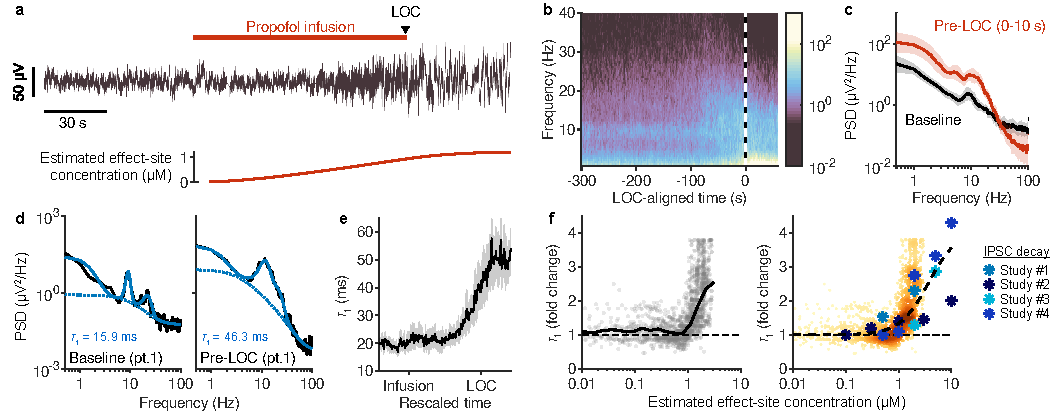
\includegraphics[width=180mm]{Figures/chapter2/figure8.pdf}}
    \centerline{
    \begin{minipage}[c]{180mm}
    \caption{\captiontitle{Model predicts and quantifies effects of propofol administration on EEG spectra.}
	\textbf{a} Representative EEG signal, Cz recording site, of a subject receiving an infusion of propofol until loss of consciousness (LOC). The estimated effect-site concentration of propofol is plotted below. 
	\textbf{b} Mean LOC-aligned spectrogram of 14 subjects. 
	\textbf{c} Average power spectrum at baseline (black), averaged between 0-10 \unit{\second} prior to propofol infusion, and after propofol infusion (red), averaged between 0-10 \unit{\second} prior to LOC. Shading reflects 95\% confidence intervals of the mean (n=14 subjects). 
	\textbf{d} Representative EEG spectrum at baseline, 0-10 \unit{\second} prior to propofol infusion (left, black) and 0-10 \unit{\second} prior to LOC (right, black). Spectra have been fitted with Eq.~\ref{eq:fitting} (see Methods), using a FOOOF-like fitting algorithm\cite{Donoghue2020} that accounts for several Gaussian peaks in the spectra (solid blue). Fitted trend is shown with dashed line.
	\textbf{e} The parameter $\tau_1$, estimated from fits to spectra computed in 2-s windows, plotted with respect to rescaled time. Shading reflects 95\% confidence intervals of the mean (n=14 subjects).
	\textbf{f} Left: fold change in the estimated value of $\tau_1$ plotted against the estimated effect-site concentration of propofol. Black line marks the mean for each concentration of propofol. Right: The estimated dose-response plot from the left panel (darker colours reflect higher density of points) is superimposed with in vitro data taken from four studies: Study \#127, Study \#228, Study \#329, and Study \#429. The data values taken from these studies are presented in Table S2. The dash black line is a fitted Hill function to the data from the four studies: $EC50 = 3.7$ \unit{\micro\molar} and Hill coefficient (n) = 1.6.} 
    \label{fig:figure2.8}
    \end{minipage}
    }
\end{figure}


Our modelling results suggest that propofol inflates low frequency power by increasing the slow timescale, $\tau_1$, of the spectral trend (\autoref{fig:figure2.1}d, e; \autoref{fig:figure2.7}). To test this, we estimated $\tau_1$ from the EEG data by fitting a modified Eq.~\ref{eq:linear_model} to the EEG spectra (Eq.~\ref{eq:fitting}; see Methods). This modified function fit the spectral trend well except at frequencies less than ${\sim}3$ \unit{\hertz} (\autoref{fig:figure2.8}d; \autoref{fig:figureS2.5}a-c), where our modelling results suggest the spectral trend is coloured primarily by neural dynamics, such as delta oscillations and/or subcritical network activity, but not synaptic kinetics (Figs. 4 \& 5). Corroborating this interpretation, the low frequency ($<3$ \unit{\hertz}) part of the trend waxed and waned from second to second, occasionally disappearing entirely, whereas the fitted synaptic timescale remained stable between time windows (\autoref{fig:figureS2.5}c). The extracted timescale, $\tau_1$, was remarkably consistent prior to the infusion of propofol, with an average value of 16.7 ± 1.4 ms (mean $\pm$ SE, $n=14$) (\autoref{fig:figure2.8}e). Following the infusion of propofol, $\tau_1$ began increasing, reaching a value of 43.2 $\pm$ 4.6 \unit{\milli\second} ($p \approx 10^{-4}$; paired two-tailed t-test) 0-10 \unit{\second} prior to LOC (\autoref{fig:figure2.8}e). Similar changes were observed at other electrode sites (\autoref{fig:figureS2.6}). By plotting the estimated value of $\tau_1$ at each time point against the estimated effect-site concentration of propofol, quantified using the Marsh model \cite{Marsh1991}, we constructed a dose-response curve of fold change in $\tau_1$ against estimated propofol concentration (\autoref{fig:figure2.8}f). The inferred dose-response curve for $\tau_1$ quantitatively matched in vitro measurements of inhibitory postsynaptic current kinetics in the presence of bath applied propofol \cite{Kitamura2003, Orser1994, Whittington1996} (\autoref{fig:figure2.8}f). Thus, the changes in $\tau_1$ were consistent with expectations based on propofol’s known pharmacology. These observations support the model’s prediction that GABAR kinetics significantly shape EEG spectra and that broadband EEG changes do not necessarily reflect differences in brain dynamics. 


\subsection{Correcting for synaptic timescales reveals a unique signature of LOC}
Our modelling results predicted that propofol’s effect on synaptic timescales will produce errors in conventional quantifications of brain rhythms. Past studies have suggested that LOC from propofol is associated with changes in the delta (0.5-3 \unit{\hertz}), alpha (8-15 \unit{\hertz}), and beta (15-30 \unit{\hertz}) frequency ranges \cite{Purdon2013}. To investigate the consequences of spectral detrending on EEG signatures of LOC, we compared raw bandpower to detrended bandpower in the delta, alpha, and beta frequency ranges. To compare EEG dynamics across individuals, data were aligned simultaneously to the moment of propofol infusion and LOC; this was done by rescaling time in each experiment by the latency to LOC (median: 135 s; range: 95-285 s). Similar results were obtained when time was not rescaled (\autoref{fig:figureS2.5}d). Consistent with previous studies\cite{Purdon2013}, raw baseline-normalized power increased in the delta, alpha, and beta band following propofol infusion (\autoref{fig:figure2.9}a-c). Whereas alpha power increased quickly and plateaued prior to LOC, delta power rose slowly and continued increasing until after LOC (\autoref{fig:figure2.9}d). Notably, beta power increased concomitantly with alpha power, but then began decreasing prior to LOC, eventually producing a beta power not statistically different from baseline post-LOC (\autoref{fig:figure2.9}d). 




\begin{figure}[t!]
    \centerline{\includegraphics[width=180mm]{Figures/chapter2/figure9.pdf}}
    \centerline{
    \begin{minipage}[c]{180mm}
    \caption{\captiontitle{Correcting for synaptic timescales reveals a unique signature of losing consciousness.}
	\textbf{a} Left: representative EEG power spectrum following LOC (black) of a single subject, superimposed on the power spectrum at baseline (blue). Right: power spectrum following LOC (black) normalized to baseline. 
	\textbf{b} Mean baseline normalized spectrogram (n=14 subjects).
	\textbf{c} Average baseline-normalized power 0-10 \unit{\second} prior to LOC (shading: 95\% confidence interval of mean). Power was significantly elevated within the delta ($p=0.001$, right-tailed sign test; $n=14$ subjects), alpha ($p\approx10^{-4}$), and beta ($p=0.007$) frequency bands.
	\textbf{d} Changes in alpha, beta, and delta power, aligned to both moment of propofol infusion and LOC, averaged across subjects (shading: 95\% confidence interval of mean). Bars above graph indicate 0.05-long segments of rescaled time where there is a statistically significant increase ($p<0.05$, right-tailed sign test) in the corresponding frequency band power. \autoref{fig:figureS2.5}d shows results without rescaled time. 
	\textbf{e} Left: EEG spectrum following LOC, same as (\textbf{a}), superimposed with fitted inhibitory timescale (Eq.~\ref{eq:fitting}). Fitted Gaussian peaks not shown. Right: detrended power, defined as power relative to fitted inhibitory timescale, in decibels. 
	\textbf{f} Mean detrended spectrogram, normalized to baseline (n=14 subjects).
	\textbf{g} Detrended power 0-10 \unit{\second} prior to LOC, normalized to baseline (shading: 95\% confidence interval of mean). Power was significantly elevated within the alpha ($p= 0.006$) and beta, ($p=0.001$), but not delta ($p=0.40$) frequency bands. Significance testing same as (\textbf{c}).
	\textbf{h} Same as in (\textbf{d}), but for detrended power, normalized to baseline.} 
    \label{fig:figure2.9}
    \end{minipage}
    }
\end{figure}
 

To correct for the confounding effects of propofol, we divided EEG power at each timepoint by the estimated synaptic timescales fitted from the previous section (\autoref{fig:figure2.9}e). We then normalized detrended power by the detrended power at baseline (\autoref{fig:figure2.9}f), such that changes in bandpower reflected the spectral changes unexplained by the increase in $\tau_1$. This procedure entirely removed the apparent rotation in the EEG spectra following propofol infusion (\autoref{fig:figure2.9}g). As a result of this detrending, power in the alpha, beta, and delta bands clearly increased at distinct times (\autoref{fig:figure2.9}h). Alpha and beta power appeared following propofol infusion and plateaued well before LOC. In contrast, detrended delta power did not increase until the moment of LOC, at which point it increased sharply (\autoref{fig:figure2.9}h; \autoref{fig:figureS2.5}d). In summary, whereas the raw EEG signal failed to exhibit a strongly time-locked signal at the moment of LOC, removing the anticipated confounds of propofol revealed a sharp increase in delta power within seconds of LOC. This analysis combined with our modelling results suggest that pharmacological changes to synaptic kinetics may mask the true dynamics of neural oscillations when spectral detrending is not performed. Additionally, these results point to distinct roles for alpha and delta power in the function of propofol as a general anesthetic. 

\section{Discussion}
In this study, we explored the neural basis of the EEG spectral trend and examined its implications for EEG interpretation and analysis. Several important conclusions came out of this investigation. First, this work provided biophysical evidence that arrhythmic neural activity is capable of generating detectable EEG signals. Second, our modelling consolidated the predictions of simpler computational models \cite{Gao2017, Chaudhuri2018} and indicated that the EEG spectral trend is shaped by the interactions of many factors, including synaptic kinetics, excitatory-inhibitory ratio, and aperiodic network dynamics. Third, our analysis revealed that spectral peak amplitudes are minimally affected by fluctuations in arrhythmic neural activity. On the other hand, we found that systemic changes in synaptic current properties do necessitate detrending to accurately interpret spectral changes as variations in neural activity. Our results suggested that this latter scenario is particularly important for EEG recordings used in tandem with pharmacological interventions. 

Traditional spectral analysis assumes that EEG power within canonical frequency bands reflect various brain rhythms. Our modelling results seriously challenge this assumption. Specifically, if a spectral peak is not evident within a given frequency band, our work justifies a physiologically plausible and biophysically realistic alternative hypothesis, namely, that the bandpower reflects broadband neural activity. Our results thus validate the principle assumption of spectral detrending methods, such as the FOOOF algorithm \cite{Donoghue2020}, which is that peak detection is a necessary prerequisite to quantifying oscillatory power. While power lying outside spectral peaks could potentially reflect neural rhythms, there is no theoretical guarantee for this interpretation based on spectral analysis alone. 

Importantly, our results do not necessarily support a purely data-driven approach to detrending EEG spectra. While changes in arrhythmic activity affect spectral peaks in an additive manner (\autoref{fig:figure2.5}), changes in synaptic currents multiplicatively scale spectral peaks (\autoref{fig:figure2.7}); these two mechanisms thus require two distinct methods of detrending, i.e., subtractive versus divisive detrending, respectively. Without prior knowledge, it is unclear which method is required. Moreover, given the amplitude of peaks above the background trend typical in EEG spectra, small additive changes in the trend would alter the peak amplitudes minimally compared to the errors introduced by incorrectly detrending (\autoref{fig:figure2.5}). Overall, we conclude that spectral detrending should not be performed unless there is clear physiological and biophysical justification and validation. 

In the analysis presented here, there was prior knowledge of the well-documented action of propofol on GABAR kinetics \cite{Kitamura2003, Orser1994, Whittington1996}, clearly indicating the necessity for divisive detrending. To mitigate the chances of overfitting, we constrained parameter values to physiologically reasonable ranges, and validated that the fitted spectral changes and $\tau_1$ values quantitatively matched expectations. Even so, our decomposition of spectra into physiologically distinct components was likely imperfect, especially considering that changes to GABAR kinetics also probably affected aperiodic network dynamics \cite{Li2020} (see below). Although inhibitory synapses and network timescales are expected to affect spectra in different frequency ranges (Figs. 1, 4, 5, 7), these ranges overlap, making it challenging to definitively disambiguate these two mechanisms. Such caveats may be addressable with future refinements to EEG detrending algorithms, e.g., by including phase information or using generative models to improve parameter inference \cite{Zeraati2022}. 

Past modelling has suggested that the EEG spectral exponent reflects the E:I ratio, which relies on the assumption that low frequency power is dominated by inhibitory currents \cite{Gao2017}. Our results broadly validate this assumption, suggesting that the E:I ratio is an important driver of the spectral trend. However, our results also demonstrate that the spectral exponent is not a reliable measure of E:I ratio because of nonlinearities in membrane potential dynamics related to the reversal potentials of AMPARs and GABARs (\autoref{fig:figure2.6}), an aspect not considered in previous work \cite{Gao2017}. Additionally, we found that other biophysical parameters, such as synaptic timescales and leak currents contribute to shaping the EEG spectral trend. These findings are consistent with past studies that have associated neuronal timescales with the expression levels of various ion channels and receptor subunits \cite{Gao2020}. It seems likely that changes in the spectral trend can reflect a large number of physiological mechanisms that converge to govern synaptic kinetics and the effective E:I ratio. Other biophysical mechanisms not explored here, such as active membrane currents \cite{Reimann2013} and dendritic calcium spikes \cite{Suzuki2017}, could also potentially contribute to shaping EEG spectra by changing postsynaptic response kinetics and amplitudes. Broadly, we conclude that the spectral exponent reflects physiological factors other than neural oscillations and is therefore a complementary biomarker to brain rhythm quantification.

While several studies have suggested that avalanche criticality may be responsible for broadband $1/f^\beta$ scaling in EEG spectra \cite{Beggs2003, He2014, Lombardi2017, Petermann2009}, our results corroborate other models of recurrent neural networks \cite{Chaudhuri2018} and indicate that avalanche criticality would likely contribute to only slower frequency components of EEG (\autoref{fig:figure2.4}, in the limit as $m\rightarrow 1$). In a general sense, our model suggests an underlying mechanism for the observed $1/f$ trend comparable to that proposed for how purely oscillatory networks might produce such a trend. In the oscillatory case, it has been suggested that large networks oscillate slower than smaller networks, thus leading to a $1/f$ trend \cite{Buzsaki2004, Buzsaki2023}. Our results suggest that propagating spikes that exhibit longer correlation timescales can produce more coherent dipoles, thus contributing more to the EEG signal. This in turn would cause EEG spectra to be dominated by lower frequency aperiodic signals. While still technically challenging, our model could be tested by extending recent work characterizing the functional clustering of synapses within individual dendritic branches \cite{Iacaruso2017, Ju2020, Kerlin2019, Lafourcade2022}, and by measuring the geometric relations between correlated synapses across neighbouring neurons.

Delta rhythms are a ubiquitous feature of general anesthesia, being readily induced in humans by propofol, sevoflurane, thiopental, and xenon\cite{Purdon2013, Gugino2001, Huupponen2008, Johnson2003, Lewis2012, Ma2006, Murphy2011}, potentially indicating a universal signature of unconsciousness bridging both general anesthesia and sleep \cite{Amzica1998, LeMasson2002, Steriade2000}. To the best of our knowledge, such an abrupt change in delta power as reported here has not been previously reported in EEG studies, even when the moment of LOC was resolved with high temporal precision\cite{Purdon2013}. Although practically detrending power relies on simplified models of EEG spectra, our analysis clearly shows that the slow changes in delta power prior to LOC can be explained by propofol’s action on GABAR kinetics, and thus demonstrates that delta power originating from changes in neural dynamics appears after the propofol-induced increase in alpha and beta power (\autoref{fig:figure2.9}). According to our simulations, it is possible that the observed increase in low frequency power is due to the brain moving closer to avalanche criticality (Figs. \ref{fig:figure2.4} \& \ref{fig:figure2.5}). Opposing this interpretation are models of excitatory/inhibitory networks, which suggest that increasing inhibition promotes the asynchronous state \cite{Li2020}. Furthermore, detailed analyses of EEG signals have suggested that altered states of consciousness are related to a departure away from, and not towards, critical dynamics \cite{Tagliazucchi2016, Toker2022}. Based on these studies, we should rather expect changes in network criticality that decrease delta power. It seems likely, therefore, that the increase in delta power at the moment of LOC is related to changes in delta rhythms. If so, our observations lend evidence to the view that delta rhythms are fundamental to losing consciousness. A target effect-site concentration protocol could be used to investigate lower doses of propofol in more detail, which our observations suggest may induce alpha rhythms but not delta rhythms. If so, these experiments could be used to dissect the behavioral correlates of these two rhythms in more detail.

In summary, we conclude that aperiodic neural activity can contribute to EEG signals, and that the spectral trend is further shaped by many physiological mechanisms, such as excitatory/inhibitory balance and synaptic timescales. We conclude that the spectral exponent is not merely a conflated measure of brain rhythms and thus provides a complementary biomarker of brain state. However, we also conclude that the spectral exponent does not have a singular physiological interpretation. Finally, we conclude that EEG spectra do need to be detrended when quantifying brain rhythms, but only if postsynaptic current properties are systematically altered. Otherwise, detrending likely introduces significant errors to brain rhythm quantification and should therefore be avoided.

\section{Methods}
\subsection{Definitions and theoretical framework}
The EEG signal can be described as the linear superposition of electric fields generated by all neurons in the brain \cite{Nunez2006,Malmivuo1995}. We refer to the individual contribution of a single neuron to the ensemble EEG signal as a single-neuron EEG. Otherwise stated, the ensemble EEG signal is the linear summation of N single-neuron EEGs. This means that the power spectral density of an EEG signal can be expressed as
\begin{equation} \label{eq:superposition}
S_N(f)=\sum_{i}{S_i(f)}+2\sum_{i<j}{\gamma_{ij}\left(f\right)\sqrt{S_i S_j}}
\end{equation}
Here, $S_i$ is the power spectrum of the single-neuron EEG generated by a given neuron i, and $\gamma_{ij}$ is the coherence between the single-neuron EEG of neuron i and neuron j. Spectral peaks are thought to appear due to coherence at a given frequency \cite{Nunez2006}. Because the coherence function, $\gamma_{ij}$, interacts multiplicatively with single neuron EEG spectra, the spectral features of the ensemble EEG will be governed in part by the spectral features imparted by neurons at the single cell level. Moreover, this influence will be independent of the nature of brain dynamics, except insofar as these dynamics alter the single-neuron EEG spectrum. Broadly, this paper concerns itself with investigating how broadband single-neuron EEG signals influence the spectral features of the ensemble EEG. 

\subsection{Postsynaptic neuron simulations}
Neuron morphologies as well as their relative abundance were the same as those used by Hagen \textit{et al.} \cite{Hagen2016} (Table S1). The same biophysical parameters were used for all neuron subtypes. For simulations, morphologies were segmented such that each compartment was less than \qty{10}{\micro\meter}. Each postsynaptic neuron was modelled with an axial resistance $R_a=100$ \unit{\ohm \centi\meter} and a membrane capacitance of 1 \unit{\micro\farad\per\centi\meter\squared}. All compartments were passive. The maximal leak conductance ($g_L$) was investigated in a range from 0.01 to \qty{5}{\milli\siemens\per\centi\meter\squared} and the leak reversal potential ($E_L$) was investigated in a range from -75 to -45 \unit{\milli\volt} (\autoref{fig:figure2.1}g). The number of synapses for each cell was equal to the total dendritic length times a density of 1 synapse per \unit{\micro\meter} for excitatory synapses and 0.15 synapses per \unit{\micro\meter} for inhibitory synapses \cite{Iacaruso2017, Karimi2020, Palmer2012}. Synapses were distributed among all compartments proportionally to the compartments’ surface area. Post-synaptic currents were modelled as the difference of exponentials. Excitatory synapses had a reversal potential of 0 \unit{\milli\volt}, a rise time of 0.3 ms, a decay time constant ($\tau_E$) between 1 and 3.5 ms, and a peak conductance ($g_E$) between 0.2 and 2 \unit{\nano\siemens} (\autoref{fig:figure2.1}g). Inhibitory synapses had a reversal potential of -80 \unit{\milli\volt}, a rise time of 2 ms, a decay time constant ($\tau_I$) between 5 and 20 ms, and a peak conductance ($g_I$) between 0.2 and 2 \unit{\nano\siemens} (\autoref{fig:figure2.1}g). For illustrating specific example spectra, e.g., those shown in Figs. 1d, 2f, 4f, 4g, 5 and 7, the following parameter set was used: $g_L = 1$ \unit{\milli\siemens\per\centi\meter\squared}, $E_L = -58$ \unit{\milli\volt}, $\tau_E = 1.8$ ms, $g_E = 0.7$ \unit{\nano\siemens}, $\tau_I = 10$ \unit{\milli\second}, and $g_I = 0.7$ \unit{\nano\siemens}. All simulations of neurons were performed in Python 3.8.10 using the package LFPy 2.2.4 \cite{Hagen2018}, running the NEURON simulation environment under the hood \cite{Carnevale2006}.

\subsection{Ensemble EEG amplitude estimation}
Because dipoles sum linearly, the EEG signal generated by N neurons can be decomposed as a superposition of N single-neuron EEG signals. It follows that the ensemble EEG will have an average power of $\sigma_N^2=\sum_{i=1}^{N}\sigma_i^2+2\sum_{i<j}{\rho_{ij}\sigma_i\sigma_j}$, where the single-neuron EEG signals produced by neurons i and j have average powers of $\sigma_i^2$ and $\sigma_j^2$, respectively, and a pairwise correlation of $\rho_{ij}$. Dipole correlations should arise if two conditions are satisfied: (1) synaptic inputs are correlated, which we assumed to decrease with distance; and (2) dipole orientations are aligned, which we assumed depends on both condition 1 and on the angle between the apical-basal axes of the neurons. We therefore modelled the dipole correlation of two neurons as $\rho_{ij}=\exp{\left(-d_{ij}^2/\sigma^2\right)}\cos{\theta_{ij}}$, where $d_{ij}$ is the distance between the two neurons, $\sigma$ is some characteristic spatial scale of correlation, and $\theta_{ij}$ is the angle between the apical-basal axes of the respective neurons. We estimated these parameters using the ICBM152 v6 anatomical brain template \cite{Huang2016,Fonov2009,Fonov2011}, assuming a uniform density of $\mu = 100,000$ neurons per \unit{\milli\meter\squared} of cortical surface area \cite{Carlo2013}.

The brain template is a triangular mesh with faces of areas $A_j$ and normal vectors ${\vec{N}}_j$. Given a random point, $x_i$, on the mesh, we used the vertex points of the mesh to analytically calculate the “signed number” of neurons within a given radius $r$, given by 
\begin{equation}
\nu_i\left(r\right)=\sum_{j}{\mu\left(A_jf_j\left(r,x_i\right)\right){\vec{N}}_j\cdot{\vec{N}}_i}
\end{equation}
where $f_j\left(r,x_i\right)$ is the fraction of triangular mesh face $j$ that intersects a ball of radius $r$ centered at point $x_i$. We repeated this $k=2000$ times with different starting points, $x_i$, to estimate an average $\bar{\nu}\left(r\right)=\frac{1}{k}\sum_{k}{\nu_i(r)}$. This allowed us to estimate the average pairwise correlation across the entire cortex with the following formula 
\begin{equation}
\bar{\rho}=\frac{1}{N-1}\int_{r>0}{\exp{\left(-r^2/\sigma^2\right)}d\bar{\nu}\left(r\right)}
\end{equation}
It follows that the expected signal power of the ensemble EEG signal is $\sigma_N^2=N\sigma_0^2+N\left(N-1\right)\bar{\rho}\sigma_0^2$, where $\sigma_0^2$ is the expected power of a single-neuron EEG (\autoref{fig:figure2.1}).
Experimental quantification of $\sigma^2$ would require measuring and comparing the isolated dipoles of individual neurons, a procedure that is not possible. However, correlations in subthreshold membrane potentials have been investigated in cats, both in the presence and absence of oscillations \cite{Volgushev2011}. These experiments revealed that in the absence of oscillations, subthreshold fluctuations were correlated between neocortical neurons up to ${\sim}5$ mm apart, but were uncorrelated between neurons ${\sim}13$ \unit{\milli\meter} apart \cite{Volgushev2011}. Because dipoles are predominantly generated by subthreshold currents \cite{Buzsaki2012, Einevoll2013}, these data suggest a possible lower and upper bound for $\sigma^2$.

\subsection{Subcritical network model}
Presynaptic neurons were connected to $d_{out}=10$ other neurons in the presynaptic network. The probability of two neurons being connected was determined by their distance, using an exponentially decaying coupling kernel. This rule forced network connectivity to be local in nature. Each neuron followed a Poisson point process with a rate $\lambda_E (1-m)$, where $\lambda_E$ was sampled from the distribution shown in \autoref{fig:figure2.1}g. When a neuron spiked, each of its neighbouring neurons had a probability of $m/d_{out}$ of firing an action potential within the following \qty{4}{\milli\second} \cite{Wilting2019}. The parameter $m$ thus tuned the amount of spike propagation in the network, changing the network behaviour from completely asynchronous when $m=0$, to near avalanche criticality as m approached 1. The above formalism was used to simulate excitatory presynaptic neurons. We also added inhibitory neurons totaling 15\% of the entire network. Spike trains for inhibitory neurons were sampled from the spike trains of nearby excitatory neurons and supplemented with independent Poisson processes. The procedure was such that inhibitory neuron firing was driven by recurrent connections to the same proportion as excitatory neurons and followed a predetermined firing rate ($\lambda_I$). In this setup, the influence of inhibitory neurons on the network was modelled implicitly in the branching number \cite{Li2020}, but were not explicitly represented in the network connections. This simplification allowed the effective branching number of the network to be entirely governed by a single parameter $m$. 

\subsection{Embedding synapses onto postsynaptic dendrites}
Dipole synchrony has been previously modelled either by separating inhibitory and excitatory input into somatic and apical compartments, respectively \cite{Nunez2006}, or by having counterphase input into the basal and apical compartments \cite{Jones2009, Studenova2022}; both of these models can be thought of as optimal mappings of two anticorrelated populations of synapses. Inspired by these models, we developed a procedure to generate dipole synchrony given any presynaptic topology. First, the pairwise correlation between each pair of presynaptic neurons was determined by the spike time tiling coefficient (STTC) \cite{Cutts2014}, a measure of spike train correlation which accounts for the likelihood of spikes overlapping by chance. The pairwise correlations among all presynaptic neurons were computed based on \qty{40}{\second} long simulations of the presynaptic networks. The Uniform Manifold Approximation and Projection (UMAP) algorithm, a dimensionality reduction technique\cite{McInnes2018}, was then used to optimally project the presynaptic network onto a sphere such that the angle between presynaptic neurons with high STTCs was minimized. After this embedding step, the dendrites of the postsynaptic neurons were orthogonally projected onto the sphere. Finally, the following procedure was run until all connections were formed between pre- and post-synaptic neurons: (1) a postsynaptic dendrite segment was chosen randomly (with replacement) with a probability proportional to its surface area; (2) the presynaptic neuron closest on the spherical embedding was chosen and a connection formed.

To model suboptimal synapse placement, we randomly perturbed the spherical embedding before mapping the synapses. Each point in the embedding was perturbed by a distance \[\pi\arccos {(1-2\alpha\left(1-X\right))}\] along a randomly chosen bearing, where $\alpha\sim \mathrm{Uniform}[0,1]$.Here, $X$ is what we refer to as the optimality index (\autoref{fig:figure2.4}e). By construction, when $X=1$, the points on the sphere are not perturbed at all, while when $X=0$, all the points on the sphere are perturbed by a distance sampled from the function $\pi\arccos{(1-2\alpha)}$. Consequently, for $X=0$, the distribution of points on the sphere is uniformly random.

This procedure can be thought of as a model of dipole correlation that generalizes beyond dichotomous input. Alternatively, this procedure can be considered in terms of observations from recent studies, which have reported that functionally related synaptic inputs cluster within individual dendritic branches, and that input from similar presynaptic populations target similar dendritic compartments in the postsynaptic population \cite{Iacaruso2017, Ju2020, Kerlin2019, Lafourcade2022, Scholl2017}. These experimental observations hint at a more continuous mapping of synaptic input along dendrites than a strictly binary apical-basal compartment paradigm, which is precisely what is achieved when the above mapping algorithm is applied to a continuous presynaptic network topology, such as the planar subcritical network used in \autoref{fig:figure2.5}.

\subsection{Mixed synaptic input}
For modelling oscillatory input, we used a published formalism of rhythmogenesis, where counterphase sinusoidal inputs were applied on the apical and basal dendrites \cite{Jones2009, Studenova2022}. Specifically, every synapse on the neuron received an inhomogeneous Poisson point process as input, with a rate function $\lambda_x\left(1+\alpha_R\sin{\left(2\pi\omega t+k\right)}\right)$, where $\lambda_x$ depends on whether the synapse is excitatory ($\lambda_E$) or inhibitory ($\lambda_I$), $\alpha_R$ tunes the strength of the rhythm, and $k=\pi$ for apical dendritic synapses and k=0 for basal dendritic synapses. For simplicity, to model other rhythms, we generalized this formalism by defining the rate function of each synapse as $\max{\left(\lambda_x\left(1+\alpha\widetilde{Y}{\left(t\right)}\right),0\right)}$, where $\widetilde{Y}=Y(t)$ if the synapse was an apical synapse and $\widetilde{Y}=1-Y(t)$ if the synapse was a basal synapse, for any time series $Y(t)$ with zero mean and unit variance. This methodology was simpler than modelling networks for each type of dynamic and embedding the synapses as described in the above section, but more importantly this methodology allowed us to make direct comparisons between the modelled EEG signals generated by different rate functions.

\subsection{Experimental design and procedure}
Following MNH Ethics Board approval, we recruited 16 American Society of Anesthesiologists (ASA) class I or II patients (18-65 years old) presenting for lumbar disk surgery as subjects for the study. All subjects gave written informed consent to participate in the study. The standards of care of the Canadian Anesthesiologists' Society in regard to monitoring, equipment and care provider were rigorously applied. Gold cup electrodes (Fz, Cz, Pz, C3, C4, CP3, CP4, M2 as reference; FC1 as ground; impedance $\le5$ \unit{\kilo\ohm}) were glued to the scalp to obtain a continuous EEG recording, which was amplified with a 0.1-300 \unit{\hertz} band pass and digitized at 1024 \unit{\hertz}. For each participant, we obtained 2 minutes of recording during preoxygenation with eyes closed. The participant was then asked to hold an object (\qty{0.5}{\kilo\gram} cylinder; \qty{2.5}{\centi\meter} diameter and 15 \unit{\centi\meter} long) in a vertical position with their dominant hand and to keep the eyes closed. Preoxygenation continued for another \qty{2}{\min}. Lidocaine 2\% (40 \unit{\milli\gram}) was given to attenuate the discomfort caused by the propofol injection. All medications were given intravenously via a catheter placed on the non-dominant arm. Propofol was given at the rate of 1 \unit{\milli\gram\per\kilo\gram\per\minute} and maintained until the cylinder fell from the participant’s hand. Following LOC, gentle jaw lift was applied if needed to relieve airway obstruction. The ability of the participants to respond to loud verbal command was assessed \qty{60}{\second} after the fall of the object: all failed to response and remained immobile. The study was then terminated. 

\subsection{Data analysis}
Two participants were excluded because of failure to comply with the instructions during induction. One kept talking, the other kept moving their dominant arm. The final data set was therefore based on 14 subjects (10 males; 12 right-handed). Artifacts in the data were removed following visual inspections of the time series. Spectrograms were computed with the multitaper method, using three tapers over \qty{2}{\second} windows, with \qty{1.9}{\second} overlap. Group averages were either computed as the average power spectral density across subjects with time aligned to LOC, or with time rescaled so that both the infusion onset and LOC were aligned across individuals. To rescale time, LOC-aligned time for each subject was scale by the latency from infusion to LOC. Consequently, a rescaled time value of $-1$ is equivalent to the moment of propofol infusion onset and a rescaled time value of 0 is equivalent to the moment of LOC. 

\subsection{Estimated propofol concentration}
For estimating the effect-site concentration of propofol for each subject, we used the Marsh model, a multicompartment pharmacokinetics model \cite{Marsh1991}. We used a plasma to effect-site equilibration rate constant $k_{eo}=1.21$ \unit{\per\minute} ~\cite{Struys2000}. Faster and slower values for $k_{eo}$ would shift the estimated dose-response curve in \autoref{fig:figure2.8}f right and left, respectively, but would not be expected to qualitatively change our results.

\subsection{Detrending EEG spectra}
To detrend EEG spectra, we used a modified version of the FOOOF algorithm\cite{Donoghue2020}, whereby a background trend is fitted in addition to several Gaussian functions to account for oscillatory peaks. Peaks at 60 \unit{\hertz} due to noise were removed from spectra using MATLAB’s fillgaps function prior to fitting the spectral trend. The FOOOF algorithm provides two options for the background trend, $A/f^\beta$ or $A/\left(k+f^\beta\right)$. Here, we wanted a biophysically interpretable background function, and therefore started with the sum of two Lorentzian functions (Eq.~\ref{eq:linear_model}). This function is an exact analytical solution to the computational model of Gao \textit{et al.} \cite{Gao2017} and has several benefits. Firstly, it provides exact solutions to our simulations, which allowed us to investigate theoretical consequences of detrending EEG spectra. Secondly, the parameters are physiologically interpretable. $\tau_1$ and $\tau_2$ reflect the kinetics of GABARs and AMPARs (\autoref{fig:figure2.1}), while $A_1$ and $A_2$ reflect the amplitudes of inhibitory and excitatory contributions to the EEG signal. Thirdly, it is thought that the spectral exponent, $\beta$, reflects the relative contribution of excitation to inhibition \cite{Gao2017}, i.e., it depends on the ratio of $A_1$ to $A_2$ (\autoref{fig:figure2.1}). However, we found here that this is not always the case (\autoref{fig:figure2.6}). Therefore, Eq.~\ref{eq:linear_model} makes fewer assumptions about its parameters than the two options provided by the FOOOF package.

For analyzing experimental data, we modified Eq.~\ref{eq:linear_model} to provide better fits to the data and reduce the chances of overfitting. In contrast to our simulations, we found that high frequency power plateaued in our data around where we would expect the influence of excitatory synaptic time scales to be exerted (\autoref{fig:figure2.1}d, f). We therefore replaced the second term in the equation with a constant term,
\begin{equation}\label{eq:fitting_no_tau2}
A_1\tau_1/\left(1+\left(2\pi\tau_1f\right)^2\right)+\lambda    
\end{equation}
This constant term, $\lambda$, captures the fast excitatory time scales as well as any high frequency contributions from action potentials \cite{Buzsaki2012}, muscle activity \cite{Muthukumaraswamy2013}, and amplifier noise \cite{Miller2009}, which were not present in our simulations.  Importantly, because this equation has physiologically interpretable parameters, with $\tau_1$ reflecting inhibitory synaptic time scales (\autoref{fig:figure2.1}d, e), we could constrain the range of $\tau_1 $to avoid overfitting. Specifically, we constrained $\tau_1$ to be greater than 10 ms and less than 75 ms when fitting propofol data, as we expected propofol to increase the physiological range of GABAR kinetics (Table S2). 

This modified equation fit the EEG spectra at baseline conditions well, but following propofol infusion, the equation did not decay fast enough to capture the EEG spectra (\autoref{fig:figureS2.7}). This was seemingly because the original equations oversimplified the kinetics of inhibitory synapses. Notably, Eq.~\ref{eq:linear_model} is an analytical solution for exponentially decaying synaptic responses, whereas real synaptic responses are characterized by a rise time and decay time: $\exp{\left(-t/\tau_1\right)}-\exp\left(-t/\tau_r\right)$. It follows that a more accurate synaptic response function for the power spectrum is given by
\begin{equation}\label{eq:fitting}
\frac{A_1\left(\tau_r-\tau_1\right)^2}{\left(1+\left(2\pi\tau_rf\right)^2\right)\left(1+\left(2\pi\tau_1f\right)^2\right)}+\lambda
\end{equation}
where the first term is the analytical solution to the power spectrum of the difference of exponentials. $\tau_r$ is the risetime of inhibitory synaptic currents, which we fixed at $\tau_r=4$ ms to keep the number of fitting parameters low \cite{Sceniak2008}. Notably, if we fixed both $\tau_r=4$ ms and $\tau_1=20$ ms, physiologically plausible values \cite{Sceniak2008}, all our baseline data could be captured by simply changing $A_1$ and $\lambda$ (\autoref{fig:figureS2.5}a). Moreover, fitting Eq.~\ref{eq:fitting} provided consistent and physiologically plausible estimates for $\tau_1$ both at baseline and following propofol infusion (\autoref{fig:figure2.8}e, f). Thus, Eq.~\ref{eq:fitting} is biophysically motivated, physiologically interpretable, has only three parameters to fit, and captured our data well both at baseline and following the infusion of propofol (\autoref{fig:figure2.8}d; \autoref{fig:figureS2.5}a-c). 

\section{Data availability}
Computed EEG spectrograms for all subjects have been uploaded to Figshare\cite{Brake2023} (\url{https://doi.org/10.6084/m9.figshare.24777990}), along with all the simulation results required to reproduce our figures. Source data are provided with this paper.

\section{Code availability}
Code used to run simulations, analyze data, and generate manuscript figures\cite{niklas_brake_2023_10359818} has been deposited in Zenodo (\url{https://doi.org/10.5281/zenodo.10359818}) and is also available on GitHub (github.com/niklasbrake/EEG\_modelling).



\section{Acknowledgements}
This work was supported by the Natural Sciences and Engineering Research Council of Canada (NSERC) discovery grant (RGPIN-2019-04520) to AK. NB was supported by the NSERC-CREATE in Complex Dynamics Graduate Scholarship and the Fonds de recherche du Québec – Nature et technologies (FRQNT) doctoral training scholarship. The funders had no role in study design, data collection and analysis, decision to publish, or preparation of the manuscript. 

\section{Author contributions}
Conceptualization: NB, GP \& AK. Data curation: NB \& GP. Formal analysis: NB. Funding acquisition: AK \& GP. Investigation: NB, FD, AR, FA, SS \& GP. Methodology: NB. Project administration: AK \& GP. Software: NB. Supervision: AK \& GP. Visualization: NB. Writing – original draft: NB. Writing – review \& editing: NB, AK \& GP.

\section{Competing interests}
The authors have no competing interests to disclose.

\clearpage

\section{Supplementary information}

\renewcommand{\thefigure}{S\thechapter.\arabic{figure}}
\renewcommand{\figurename}{Supplementary Fig.}
\setcounter{figure}{0}

\renewcommand{\thetable}{S\thechapter.\arabic{table}}
\renewcommand{\tablename}{Supplementary Table}
\setcounter{table}{0}

\subsection{Supplementary figures}

\centerline{\includegraphics[width=180mm]{Figures/chapter2/figureS1.png}}
\centerline{
\begin{minipage}[c]{180mm}
\captionof{figure}{\captiontitle{Relationships between synapse orientation and dipole orientation.}
Dipole moments were simulated following a single synapse activation at various locations across the 11 representative neuron morphologies (Table S1). For each morphology, two plots are shown: the left plots show the azimuth of the dipole moment plotted against that of the synapse that was activated; the right plots show the elevations. Red dots reflect excitatory synapses and blue dots reflect inhibitory synapses. Unity lines are drawn in black.} 
\label{fig:figureS2.1}
\end{minipage}
}
\newpage




\centerline{\includegraphics[width=170mm]{Figures/chapter2/figureS2.png}}
\centerline{
\begin{minipage}[c]{170mm}
\captionof{figure}{\captiontitle{Effects of excitatory-inhibitory ratio on membrane potential and spectral slope depend on leak conductance.}
\textbf{a} Left: histogram of E:I ratios across 20,000 simulations with parameters sampled from the distributions in Fig. 6a. Simulations were binned into five categories, from low to high $\lambda_E$:$\lambda_I$ ratios. Middle: histogram of somatic membrane potential for simulations with a low leak conductance ($g_L < 1$ \unit{\milli\siemens\per\centi\meter\squared}), divided into the five E:I ratio categories. The average membrane potential is not largely affected by the E:I ratio in this high leak conductance condition. Right: histogram of somatic membrane potential for simulations with a high leak conductance ($g_L > 1$ \unit{\milli\siemens\per\centi\meter\squared}). A high E:I ratio significantly shifts the distribution of membrane potential to more hyperpolarized values. Blue and red vertical lines show the reversal potential of GABARs and AMARs, respectively.
\textbf{b} Same as Fig. \ref{fig:figure2.6}e, but for the slope computed between 30-50 Hz for $g_L$ high ($\rho=0.24$; $R^2=0.06$; $p<10^{-6}$; $n=5184$ simulations) and $g_L$ low ($\rho=-0.23;$ $R^2=0.05$; $p<10^{-6}$; $n=7366$ simulations).
\textbf{c} Same as \ref{fig:figure2.6}e, but with the E:I ratio defined as the ratio between $g_E$ and $g_I$ , for $g_L$  high ($\rho=0.50$; $R^2=0.25$; $p<10^{-6}$; $n=5184$ simulations) and $g_L$ low ($\rho=0.13$; $R^2=0.02$; $p<10^{-6}$; $n=7366$ simulations).} 
\label{fig:figureS2.2}
\end{minipage}
}
\newpage


\centerline{\includegraphics[width=180mm]{Figures/chapter2/figureS3.png}}
\centerline{
\begin{minipage}[c]{180mm}
\captionof{figure}{\captiontitle{Biophysical parameters alter broadband EEG properties across many types of dynamics.}
\textbf{a1}-\textbf{a5}	Five examples of synaptic input dynamics, generated by asynchronous white noise (\textbf{1}), a subcritical branching process (\textbf{2}), a recurrent Ising model \cite{Lombardi2023} (\textbf{3}), an underdamped second-order linear system (\textbf{4}), and a sine wave (\textbf{5}). $\alpha_x=0.1$ for all simulations in this figure.
\textbf{b1}-\textbf{b5}	Power spectra of the rate functions for each type of synaptic input depicted in (\textbf{a1}-\textbf{a5}), respectively. 
\textbf{c1}-\textbf{c5}	Unitary spectra associated with input depicted in \textbf{a1}-\textbf{5}, before and after changes to a biophysical parameter, including $\tau_I$ that was increased from \qty{10}{\milli\second} (black) to 30~\unit{\milli\second} (red) in the first column, $E_L$ that was increased from \qty{-60}{\milli\volt} (black) to \qty{-45}{\milli\volt} (red) in the second column, and $g_E$ and $g_I$ that were increased from \qty{0.7}{\nano\siemens} (black) to \qty{1.4}{\nano\siemens} (red) in the third and fourth columns, respectively.
.} 
\label{fig:figureS2.3}
\end{minipage}
}
\newpage


\centerline{\includegraphics[width=150mm]{Figures/chapter2/figureS4.png}}
\centerline{
\begin{minipage}[c]{\textwidth}
\captionof{figure}{\captiontitle{Detrending with Lorentzian function corrects for changes in biophysical parameters.}
\textbf{a}	Unitary spectra from Fig. \ref{fig:figureS2.3}, fit with the sum of two Lorentzian functions (Eq. 1; solid gray lines). The leftmost column shows the unitary spectrum with default parameters. The Lorentzian fit for the default parameters are also displayed in the plots in the other columns as a dashed grey line.
\textbf{b}	Unitary spectra from (\textbf{a}), detrended by dividing by the fitted Lorentzian function (solid gray lines). Colours correspond to the various parameter changes from (\textbf{a}). Note that, for each type of input dynamics, the detrended spectra have similar profiles, i.e., the effects of the parameter changes have been corrected.} 
\label{fig:figureS2.4}
\end{minipage}
}
\newpage


\centerline{\includegraphics[width=180mm]{Figures/chapter2/figureS5.png}}
\centerline{
\begin{minipage}[c]{180mm}
\captionof{figure}{\captiontitle{Spectral changes with respect to LOC-aligned time.}
\textbf{a} Top: example fits to the average EEG spectrum of each patient at baseline using Eq. \ref{eq:fitting}, while fixing the parameters $\tau_r=4$ \unit{\milli\second} and $\tau_1=20$ \unit{\milli\second}. Note the difference between the fitted Eq. \ref{eq:fitting} and the low frequency power ($< 3$ \unit{\hertz}), which our model predicts is caused by neural dynamics and not synaptic timescales. This low frequency power was fit here with a Gaussian peak function as per the FOOOF methods \cite{Donoghue2020}  fits not shown). Bottom: detrended power in decibels.
\textbf{b} Same as a, but for fits to spectra -10 to 0~\unit{\second} prior to LOC. Here, $\tau_1$   was not fixed and its estimated value for each patient is printed in blue.
\textbf{c} Example EEG from patient 13, split into five, 2 s windows (top). The power spectrum of each window is shown below, along with the fitted synaptic timescales (Eq. \ref{eq:fitting}) in red. 
\textbf{d} Same as Fig. \ref{fig:figure2.9}d \& h, but band power is plotted here against time relative to LOC. Data plotted as mean and shading represents 95\% confidence interval of mean.} 
\label{fig:figureS2.5}
\end{minipage}
}
\newpage

 
\begin{minipage}{\linewidth}
    \centerline{\includegraphics[width=120mm]{Figures/chapter2/figureS6.png}}
    \centerline{
    \begin{minipage}[c]{\textwidth}
    \captionof{figure}{\captiontitle{Changes in estimated $\tau_1$ exhibit similar dynamics across recording locations.}
    The plot labelled Cz is identical to Fig. \ref{fig:figure2.8}e. The other plots show the dynamics of $\tau_1$ for the other EEG channels. For each plot, the corresponding recording site is printed above.} 
    \label{fig:figureS2.6}
    \end{minipage}
    }
\end{minipage}
 

 \begin{minipage}{\linewidth}
    \centerline{\includegraphics[width=77mm]{Figures/chapter2/figureS7.png}}
    \centerline{
    \begin{minipage}[c]{\textwidth}
    \captionof{figure}{\captiontitle{Simple exponential decaying synaptic response does not capture spectral trend following propofol infusion.}
    \textbf{a} Example spectrum of subject 1 at baseline, same as in Fig. \ref{fig:figure2.8}d. Blue line: data fitted with Eq. \ref{eq:fitting_no_tau2}; $\tau_1=20$ \unit{\milli\second}, $A_1=56$, and $\lambda=0.034$. Red line: data fitted with Eq. \ref{eq:fitting}; $\tau_1=20$ \unit{\milli\second}, $\tau_2=4$ \unit{\milli\second}, $A_1=4470$, and $\lambda=0.043$.
    \textbf{b} Example spectrum of subject 1 following propofol infusion, 0 to 10 s prior to LOC, same as in Fig. \ref{fig:figure2.8}d. Blue line: data fitted with Eq. \ref{eq:fitting_no_tau2}; $\tau_1=46$ \unit{\milli\second}, $A_1=158$, and $\lambda=0.0026$. Red line: data fitted with Eq. \ref{eq:fitting}; $\tau_1=46$ \unit{\milli\second}, $\tau_2=4$ \unit{\milli\second}, $A_1=4570$, and $\lambda=0.0051$. Note that the blue line is not steep enough to capture the drop-off in power around \qty{30}{\hertz}.
} 
    \label{fig:figureS2.7}
    \end{minipage}
    }
\end{minipage}

\newpage

\subsection{Supplementary tables}

\begin{minipage}{\linewidth}
    \captionof{table}{\captiontitle{Representative neuron morphologies used in the model\textsuperscript{a}.}}
    \label{tab:tableS2.1}
    \vskip-\abovecaptionskip
    \vskip+\belowcaptionskip
    \small
    % \centering
    \begin{tabular}{lrlll}
        \hline
        \textbf{Cell type} & \textbf{Abundance (\%)}  & \textbf{Internal ID} & \textbf{External IDs}\textsuperscript{b} & \textbf{References} \\
        \hline
        Layer 2/3 pyramidal cell            &  26.8 &  L23E\_oi24py1      &  NMO\_10045   & Ref. \citen{Budd2010}  \\
        Layer 2/3 interneuron               &   7.5 &  L23I\_oi38lbc1     &  -           & Ref. \citen{Stepanyants2008} \\
        Layer 4 excitatory stellate cell    &  19.0 &  L4E\_j7\_L4stellate &  NMO\_00905   & Ref. \citen{Mainen1996} \\
        Layer 4 pyramidal cell              &   9.5 &  L4E\_53rpy1        &  NMO\_10040   & Ref. \citen{Budd2010} \\
        Layer 4 interneuron                 &   7.1 &  L4I\_oi26rbc1      &  -           & Ref. \citen{Stepanyants2008} \\
        Layer 5 pyramidal cell              &   4.9 &  L5E\_oi15rpy4      &  NMO\_10046   & Ref. \citen{Budd2010} \\
        Layer 5 interneuron                 &   1.4 &  L5I\_oi15rbc1      &  -           & Ref. \citen{Stepanyants2008} \\
        Layer 5 tufted pyramidal cell       &   1.3 &  L5E\_j4a           &  MDB\_2488    & Ref. \citen{Mainen1996} \\
        Layer 6 excitatory cell             &  14.0 &  L6E\_51\_2a\_CNG     &  NMO\_00879   & Ref. \citen{Contreras1997} \\
        Layer 6 pyramidal cell              &   4.6 &  L6E\_oi15rpy4      &  -           & Ref. \citen{Budd2010} \\
        Layer 6 interneuron                 &   3.8 &  L6I\_oi15rbc1      &  -           & Ref. \citen{Stepanyants2008} \\
        \hline
    \end{tabular}
    \vskip-\abovecaptionskip
    \vskip+\belowcaptionskip
    \singlespacing
    \footnotesize
    \begin{flushleft}
        \textsuperscript{a}Morphologies and relative abundances were identical to Hagen \textit{et al.}\cite{Hagen2018} \\
        \textsuperscript{b}Morphologies without NeuorMoprho (NMO) or ModelDB (MDB) IDs were accessed from the code repository associated with Hagen \textit{et al.}\cite{Hagen2018} All morphology files are also supplied in the code repository associated with this paper\cite{niklas_brake_2023_10359818}.
    \end{flushleft}
\end{minipage}

\vspace{1em}

\noindent
\setlength{\tabcolsep}{2pt}
\begin{minipage}{\linewidth}
    \captionof{table}{\captiontitle{In vitro data on inhibitory synapse kinetics in the presence of propofol.}} \label{tab:tableS2.2}
    \vskip-\abovecaptionskip
    \vskip+\belowcaptionskip
    \small
    \begin{tabular}{l|rrr|rrrrr|rrrrrr|rrrrrr}
        \hline
        & \multicolumn{3}{c|}{Study \#1\textsuperscript{a}} & \multicolumn{5}{c|}{Study \#2\textsuperscript{b}} & \multicolumn{6}{c|}{Study \#3\textsuperscript{c}} & 
        \multicolumn{6}{c}{Study \#4\textsuperscript{d}} \\
        \hline
        Propofol ($\mu$M) & 0 & 0.5 & 2 & 0.1 & 0.3 & 1 & 3 & 10 & 0 & 0.5 & 1 & 2 & 5 & 10 & 0 & 0.5 & 1 & 2 & 5 & 10 \\
        $\tau$ (\unit{\milli\second}) & 19.4 & 29.6 & 44.5 & - & - & - & - & - & 17.5 & 17.5 & 19 & 48 & 58 & 75 & 17.5 & 17.5 & 19 & 22.5 & 50 & 75 \\
        $\tau$ (fold change) & 1 & 1.5 & 2.3 & 1 & 1.2 & 1.4 & 1.5 & 2 & 1 & 1 & 1.1 & 2.7 & 3.3 & 4.3 & 1 & 1 & 1.1 & 1.3 & 2.9 & 4.3 \\
        \hline
    \end{tabular}    
    \vskip-\abovecaptionskip
    \vskip+\belowcaptionskip
    \singlespacing
    \footnotesize
    \begin{flushleft}
        \textsuperscript{a} Inhibitory post-synaptic current (IPSC) decay time constant taken from Fig. 8 of Orser \textit{et al.} \cite{Orser1994}. \\
        \textsuperscript{b} Fold change in spontaneous IPSCs estimated from Fig. 7C of Kitamura \textit{et al.} \cite{Kitamura2003}. \\
        \textsuperscript{c} Decay time of IPSCs during slow parts of evoked trains, taken from Fig. 5 of Whittington \textit{et al.} \cite{Whittington1996}. \\
        \textsuperscript{d} Decay time of IPSCs during fast parts of evoked trains, taken from Fig. 5 of Whittington \textit{et al.} \cite{Whittington1996}. 
    \end{flushleft}
\end{minipage}

\renewcommand{\thefigure}{\thechapter.\arabic{figure}}
\renewcommand{\figurename}{Fig.}
\setcounter{figure}{0}

\renewcommand{\thetable}{\thechapter.\arabic{table}}
\renewcommand{\tablename}{Table}
\setcounter{table}{0}

\chapter{Contributions of action potentials to scalp EEG: theory and biophysical simulations}
\label{sec:apEEG}
\renewcommand{\figurename}{Fig}

The previous chapter presented biophysical simulations along with experimental observations demonstrating that the EEG spectral trend is produced largely by the timescales of synaptic currents. The work analyzed how the spectral trend should be corrected at lower frequencies ($<50$ \unit{\hertz}) where most EEG analysis is concentrated. However, the spectral trend extends to higher frequencies where rhythms of interest, including gamma rhythms and high frequency oscillations, also manifest. In this frequency range, it has been hypothesized that the spectral trend observed in macroscopic neural recordings reflects active membrane mechanisms \cite{Gao2016}, i.e., voltage-gated channels and not synaptic currents. This would imply that the spectral trend needs to be corrected differently at higher frequency ranges. 

When analyzing the effects of synapse kinetics, I found that the contributions of AMPA and GABA receptors were more or less separable (\textbf{\autoref{fig:figure2.1}} \& \ref{eq:linear_model}). This is primarily because AMPA and GABA receptors are chemically-gated channels with sensitivity to distinct ligands, glutatmate and GABA, respectively. Consequently, the channels' respond to distinct signals and the resulting currents do not affect their gating. This situation admits a significantly simplified, linear model of their contributions to EEG signals. In contrast, voltage-gated channels exhibit highly nonlinear, complex behaviours. All these channels respond to the same signal, namely changes in the membrane potential, and the currents that result from channel activation change the membrane potential, thus affecting the gating of all the other channels.

Even in isolation, voltage-gated channels exhibit surprisingly complex behaviours. The gating of voltage-gated sodium (Nav) channels is determined by the asynchronous movements of four voltage-sensing domains \cite{Ahern2016}. In work parallel to the main results of my thesis  (\autoref{sec:Nav}), my co-authors and I showed that depending on the relative speed at which these voltage-sensing domains respond to a change in membrane potential, the channel may either open and cause a large influx of sodium, or it may inactive before ever opening, a phenomenon called closed-state inactivation \cite{Brake2022,Armstrong2006}. The relative speeds are determined by the specific isoform of the Nav channel, assembly with auxiliary subunits, and most importantly, the resting membrane potential of the cell. This latter condition in particular makes it impossible to define a simple impulse-response function for voltage-gated sodium channels, a modelling step that was crucial in untangling the contributions of AMPA and GABA receptors to EEG signals. It is therefore unlikely that one can understand the EEG contributions of voltage-gated channels in the same way as AMPA and GABA receptors. I therefore did not attempt to describe the individual contributions of voltage-gated channels to the EEG signal.

Instead, I considered the unitary contributions of action potentials. The action potential reflects the combined temporal interactions of voltage-gated channels during a superthreshold depolarization of the cell's membrane potential. Because action potentials are relatively consistent all-or-none responses, I reasoned that this approach should allow one to define an impulse response function for an action potential and thus indirectly characterize the contributions of voltage-gated channels to the EEG spectrum. I accomplished this by simulating over a thousand biophysical neuron models that were generated by the Blue Brain project \cite{Markram2015} to capture the diversity of neocortical cell types and their disparate morphological and electrical properties. I then combined these simulations with a novel Monte Carlo method of EEG forward modelling to characterize the contributions of action potentials to the EEG signal. The work in this chapter is under review at \textit{eLife} and will be published alongside public reviews once they become available. This chapter is a copy of the following preprint:

\vspace{1em}
\hrule
\vspace{.5em}
\noindent
\hangindent=1cm
Brake, N. and Khadra, A. Contributions of action potentials to scalp EEG: theory and biophysical simulations. \textit{BioRxiv} [\textbf{Preprint}]. June 1, 2024. Available from: \url{https://doi.org/10.1101/2024.05.28.596262}
\vspace{.75em}
\hrule
\vspace{.65em}

\noindent
The preprint is licensed under a Creative Commons Attribution 4.0 International License, and is reproduced here with minor formatting changes. To view a copy of this licence, visit \url{http://creativecommons.org/licenses/by/4.0/}.

\newpage

\section{Abstract}
Differences in the apparent 1/f component of neural power spectra require correction depending on the underlying neural mechanisms, which remain incompletely understood. Past studies suggest that neuronal spiking produces broadband signals and shapes the spectral trend of invasive macroscopic recordings, but it is unclear to what extent action potentials (APs) influence scalp EEG. Here, we combined biophysical simulations with statistical modelling to examine the amplitude and spectral content of scalp potentials generated by the electric fields from spiking activity. We found that under physiological conditions, synchronized aperiodic spiking can account for at most 1\% of the spectral density observed in EEG recordings, suggesting that the EEG spectral trend reflects only external noise at high frequencies. Indeed, by analyzing previously published data from pharmacologically paralyzed subjects, we confirmed that the EEG spectral trend is entirely explained by synaptic timescales and electromyogram contamination. We also investigated rhythmic EEG generation, finding that APs can generate narrowband power between approximately 60 and 600 Hz, thus reaching frequencies much faster than the timescales of excitatory synaptic currents. Our results imply that different spectral detrending strategies are required for high frequency oscillations compared to slower synaptically generated EEG rhythms.


\section{Introduction}
Understanding the neural mechanisms underlying EEG generation is important for inferring changes in brain state, as well as developing methods to filter out irrelevant signals. Towards this latter aim, recent work has focused on characterizing the neural basis of broadband EEG signals and defining when and how EEG spectra need to be detrended \cite{Donoghue2020, Gerster2022, Brake2024}. Studies into the neural basis of broadband EEG have primarily focused on synaptic filtering \cite{Brake2024,Gao2017,Miller2009,Bedard2006} and low frequency, aperiodic network fluctuations \cite{Brake2024, Chaudhuri2018, Lombardi2017}. However, in addition to synaptic contributions, the spectral trend observed in invasive, large-scale neural recordings, such as the local field potential (LFP) \cite{Ray2008, Ray2011, Kayser2003} and intracranial EEG (iEEG) \cite{Vidal2010, Lachaux2005} including electrocorticography (ECoG) \cite{Podvalny2015, Miller2007, Canolty2006, Crone2006}, is believed to reflect broadband contributions from spiking activity \cite{Ray2008, Ray2011, Manning2009}, especially at frequencies above ${\sim}60$~\unit{\hertz}, the so-called high gamma range. Such high frequency broadband contributions are thought to be important for determining the slope of the $1/f$ spectral trend \cite{Gao2016}.

In comparison to invasive recording techniques, the majority of the unprocessed EEG signal above 30~\unit{\hertz} reflects muscle activity \cite{Whitham2007, Whitham2008, Fitzgibbon2013, Muthukumaraswamy2013}. Moreover, EEG is thought to be incapable of measuring APs because they are believed to be too brief and unsynchronized \cite{Nunez2006, Buzsaki2012}. Nonetheless, when muscle artifacts are corrected for, EEG recordings have displayed transients in the high gamma range \cite{Onton2009, Volker2018, Seeber2015}, similar to those observed in LFP and iEEG recordings. If such high frequency transients are indeed generated by synchronized APs, it would hold significant implication for interpreting spectral peaks and correcting for the EEG spectral trend. Interestingly, a recent biophysical modelling study showed that APs account for almost 20\% of the amplitude of single-neuron dipoles, and concluded that APs can contribute significantly to EEG rhythms \cite{Thio2023}. However, a systemic investigation into the ability of APs to produce detectable scalp potentials has not been undertaken. Additionally, the potential contribution of APs to aperiodic EEG signals and the overall spectral trend has not been explored.

In this study, we aim to address this gap by employing a quantitative approach that explores AP-generated EEG signals, a type of signal that we refer to hereafter as apEEG for brevity. To begin, we employ a combination of biophysical simulations and statistical modelling to examine the impact of single neuron properties and spike synchrony on the amplitude and spectral features of apEEG signals. Using these results, we evaluate whether apEEG can exhibit experimentally-measurable narrowband and broadband high gamma power. Our results have implications for interpreting high frequency EEG rhythms and for designing practical methods for spectral detrending.

\section{Results}

\subsection{Unitary AP response of single-neuron dipoles is approximately linear}

The contributions of an individual neuron to the electric potential measured by a distant electrode can be modelled by a single dipole vector that varies with time \cite{Næss2021, Murakami2006}. This case applies well to EEG signals due to the distance between the brain and scalp electrodes. To understand how APs contribute to EEG, we therefore first sought to characterize the contributions of APs to their respective neurons' dipoles. We simulated neuron models with detailed morphologies and distributed passive and voltage-gated ion channels on the soma, axon initial segment, and dendrites (\textbf{\autoref{fig:example_uAP}A}). To induce spiking, we bombarded the dendrites of this active model with background synaptic input, whereas to block spiking in the presence of such synaptic inputs, we set the conductance of voltage-gated sodium channels in the soma and axon initial segment to zero, obtaining a passive model that allowed us to characterize the dipole generated in the absence of firing ({\color{seccolor}\textbf{\autoref{fig:example_uAP}B}}). By subtracting the active and passive simulation results and thereafter taking the spike-triggered average of the single-neuron dipole, we estimated the unitary AP response of the electric field (\textbf{\autoref{fig:example_uAP}C}).

\begin{figure}[t!]
	\centering
	\includegraphics[width=13.2cm]{Figures/chapter3/figure1.png}
    
    \caption{\textbf{Calculating the unitary AP response.} (\textbf{A})~The extracellular electric field generated by a neuron is shown at the peak of an AP. (\textbf{B})~Left: The single-neuron dipole, $\bm{q}$, associated with the neuron in panel A for the active model (black) and passive model with sodium channels removed (grey). The x, y, and z components of the vector are plotted from top to bottom. Notice the correspondence in the subthreshold fluctuations between the two sets of simulations. Right: The power spectrum of each dipole component trace on the left for the active (black) and passive (gray) model. (\textbf{C})~Left: The difference between the single-neuron dipoles calculated with the active and passive model aligned to each AP (light blue), along with the spike-triggered average (dark blue) which defines the unitary AP response. x, y, and z components are shown from top to bottom. Right: the power spectrum of the unitary AP response. (\textbf{D})~The firing rate of the active (black) and passive (gray) model as a function of E:I ratio, defined as the ratio between the rate of excitatory synapse activation, $\lambda_E$, to that of inhibitory synapse activation, $\lambda_I$. (\textbf{E})~The power spectrum of the z component of the single-neuron dipole (black) at three different firing frequencies: 0~\unit{\hertz} (left), 3~\unit{\hertz} (middle) and 7~\unit{\hertz}(right), along with the spectra of the passive models (gray) and the spectra of the unitary AP response (blue) shown previously in panel C. Notice how the unitary AP spectrum matches, up to a scaling factor ($\beta$), the single-neuron dipole spectrum at high frequency. (\textbf{F})~The scaling factor for the unitary AP spectrum that fits the single-neuron dipole spectrum, plotted as a function of the firing rate (black dots). These data points almost align perfectly with the unity line (black line). The x and y components of the dipole vector show the same behaviour (\textbf{\autoref{fig:linear_model_xy}}).} 
    \label{fig:example_uAP}
\end{figure}

The ensemble electric field is equal to the linear summation of those generated by each individual neuron in the brain \cite{Nunez2006, Malmivuo1995}. However, the electric fields generated by individual neurons are not in general linear; sublinear and supralinear interactions among synaptic currents prevent this \cite{Tran-Van-Minh2015}. Nonetheless, one might hypothesize the contributions of APs to be linear. In this case, the spectrum of the single-neuron dipole, $S(f)$ would be proportional to the energy spectrum of the unitary AP response, $S_{ap}(f)$, satisfying the equation
\begin{equation} \label{eq:linear_spectrum}
S(f) = S_{syn}(f) + \beta S_{ap}(f),
\end{equation}
where $S_{syn}(f)$ is the power spectrum of the synaptic contributions, and $\beta$ is a scaling factor that should be equal to the cell's firing rate, as we demonstrate below. To test the accuracy of this simplified model, we calculated single-neuron dipoles while varying the firing rate of the neuron by altering the ratio of excitatory to inhibitory input (\textbf{\autoref{fig:example_uAP}D}). We estimated $S_{syn}$ for each EI ratio by considering the passive model in which the sodium channel conductance was set to zero. Meanwhile, $S_{ap}$ was defined as the energy spectrum of the unitary AP response calculated at low firing rates (see Methods). By fitting the power spectrum of the single-neuron dipole at each EI ratio with \textbf{\ref{eq:linear_spectrum}}, we estimated the scaling factor $\beta$ and showed that it closely matches the firing rate (\textbf{\autoref{fig:example_uAP}E, F}). 

We performed this analysis on biophysical models of 68 representative neuron classes \cite{Markram2015} (\textbf{Table~S1}). Across all models, the unitary AP scaling factor $\beta$ closely followed the firing rate (\textbf{\autoref{fig:all_linear_model}A}). However, as the firing rate increased, the accuracy of the linear approximation decreased (\textbf{\autoref{fig:all_linear_model}B}). This was because the unitary AP responses were less representative of the AP responses occurring at high frequencies. Nonetheless, we found that the spectral profile of the AP-generated signal was nearly identical to that predicted by the linear model up to firing rates of approximately 80~\unit{\hertz} (\textbf{\autoref{fig:all_linear_model}C}). We concluded that the amplitude of AP responses are captured well by a linear model, but that the precise spectral properties of these responses may be slightly different than those predicted by a fully linear model during sustained high frequency firing above 80~\unit{\hertz}. However, considering that the average firing rates of active neurons typically fall below \qty{60}{\hertz} \cite{Baddeley1997, Griffith1966, Shafi2007, OConnor2010}, we deemed this simplification of AP signals to be acceptable.

\begin{figure}
	\centering
	\includegraphics[width=13.2cm]{Figures/chapter3/figure2.png}
    
    \caption{\textbf{AP contributions to single-neuron dipoles are linear with firing rate.} (\textbf{A})~Fitted unitary AP scaling factor ($\beta$; see \textbf{\ref{eq:linear_spectrum}}) plotted against firing rate for 68 neuron models covering the 55 neuron classes identified by Markram et al. \cite{Markram2015} (\textbf{Table~S1}). These data points align almost perfectly with the unity line (red line). (\textbf{B})~The $R^2$ value obtained from fitting a linear model (\textbf{\ref{eq:linear_spectrum}}) to the spectra of the AP dipole response in each simulation. Notice how the line of best fit (red line) shows that \textbf{\ref{eq:linear_spectrum}} gets less accurate at high firing rate. (\textbf{C})~The spectra of the z component of the single-neuron dipoles (black), averaged across all simulations with firing rates in the specified ranges, compared to the spectra predicted from the linear model (blue). For firing rates less than 80~\unit{\hertz}, the linear model produces spectra nearly identical to the simulations. At firing rates above 80~\unit{\hertz}, there is a slight departure is spectral density around 100~\unit{\hertz}. The same results were obtained with the x and y components of the dipole (\textbf{\autoref{fig:linear_model_xy}}).} 
    \label{fig:all_linear_model}
\end{figure}


\subsection{A linear model for the spectrum of AP electric fields}
Based on the foregoing linearity assumption outlined in \textbf{\ref{eq:linear_spectrum}}, we derived a general equation for the ensemble electric fields generated by APs. In general, the potential between two electrodes can be calculated from their lead field \cite{Malmivuo1995}, $\bm{\nu}(\bm{x})$, which describes the sensitivity of the measured potential with respect to a unit dipole vector at the spatial point $\bm{x}$. Using this formalism, we can write the potential generated by $N$ neurons as 
\begin{equation}
    \phi(t) = \sum_{i=1}^N \bm{\nu}^\intercal(\bm{x}_i) \bm{q}_i(t)
\end{equation}
where $\bm{q}_i$ is the single-neuron dipole of neuron $i$, located at coordinate $\bm{x}_i$ in the brain. This equation leads to the following power spectrum for the ensemble signal
\begin{equation} \label{eq:apEEG_spectrum}
    |\hat{\phi}|^2 = \sum_{i=1}^N \bm{\nu}^\intercal(\bm{x}_i) \hat{\bm{R}}_{i,i} \bm{\nu}(\bm{x}_i) + \sum_{i\ne j} \bm{\nu}^\intercal(\bm{x}_i) \hat{\bm{R}}_{i,j}\bm{\nu}(\bm{x}_j)
\end{equation}
where $\bm{R}_{i,i}(\tau)$ is the auto-correlation matrix of the single-neuron dipole for neuron $i$, $\bm{R}_{i,j}(\tau)$ is the cross-correlation matrix for two neurons $i$ and $j$, and $\hat{\bm{R}}_{i,i}$ and $\hat{\bm{R}}_{i,i}$ denote their Fourier transforms, respectively.

We now make use of the linearity result from the previous section by describing $\bm{q}_i$ as a linear filter, $\bm{q}_i(t)=\bm{q}_i^{syn}+(\bm{q}^{ap}_i*w_i)(t)$, where the vector $\bm{q}^{ap}_i$ is the unitary AP response of neuron $i$, $w_i$ is a point process describing the spike times of the neuron, and $\bm{q}^{syn}_i$ is the synaptic component of the single-neuron dipole, assumed to be statistically independent of $\bm{q}^{ap}_i$ (\textbf{\ref{eq:linear_spectrum}}; see also Discussion). The AP component of the ensemble potential is therefore
\begin{equation} \label{eq:apEEG_spectrum2}
    |\hat{\phi}_{ap}|^2 = \sum_{i=1}^N \hat{R}_{i,i}^{spike} \bm{\nu}^\intercal(\bm{x}_i) \hat{\bm{R}}^{ap}_{i,i} \bm{\nu}(\bm{x}_i) + \sum_{i\ne j} \hat{R}^{spike}_{i,j}\bm{\nu}^\intercal(\bm{x}_i) \hat{\bm{R}}^{ap}_{i,j}\bm{\nu}(\bm{x}_j)
\end{equation}
where $\bm{R}^{ap}_{i,i}(\tau)$ is the auto-correlation matrix of the unitary AP response for neuron $i$, $\bm{R}^{ap}_{i,j}(\tau)$ is the cross-correlation matrix for two neurons $i$ and $j$, $R_{i,i}^{spike}(\tau)$ is the spike train auto-correlation of neuron $i$, $R_{i,j}^{spike}(\tau)$ is the spike train cross-correlation of neurons $i$ and $j$, and $\hat{\bm{R}}^{ap}_{i,i}, \hat{\bm{R}}^{ap}_{i,j}, \hat{R}_{i,i}^{spike}$ and $\hat{R}^{spike}_{i,j}$ denote their Fourier transforms, respectively.

We estimated the average auto- and cross-correlations between unitary AP responses based on biophysical simulations of all 1035 neuron models generated by the Blue Brain project \cite{Markram2015}. As expected, when the neurons fired APs with zero lag, their dipoles exhibited strong cross-correlations along the apical-basal axes of their respective neurons (\textbf{\autoref{fig:cross_ap_correlation}}). Interestingly, these calculations also revealed significant cross-correlations between the dipoles' apical-basal component and their azimuthal components (\textbf{\autoref{fig:cross_ap_correlation}}). This observation suggests that even neurons that are not aligned in parallel may still generate coherent electric fields during synchronous firing, thus further boosting the signals generated by populations of AP responses.

\subsection{Magnitude of apEEG depends on dendrite asymmetry}
Using the above linear model, we sought to calculate the potential measured at an EEG electrode generated by APs under various conditions. To begin, we investigated the simple case where neurons fire according to uncorrelated Poisson spike trains. In this case, $\hat{R}_{i,j}^{spike}(f)=0$ and $\hat{R}_{i,i}^{spike}(f)=\lambda_i$, although for simplicity we assumed a single average $\lambda$ for all neurons. To estimate the solution to this equation, we divided our neuron models into the 55 different morphology classes defined by Markram et al. \cite{Markram2015} (\textbf{Table~S2}). Under this scenario, the apEEG spectrum was calculated as
\begin{equation} \label{eq:apEEG_spectrum_linear}
    |\hat{\phi}_{ap}|^2 = \lambda \sum_{k=1}^M m_k S_k(f),
\end{equation}
where $S_k$ is equal to the expected EEG spectrum generated by a neuron of class $k$ firing a single AP, and $m_k$ is the number of neurons that fall into each class. $S_k$ was calculated by averaging the EEG spectra generated by simulating many neurons of class $k$ and placing them at each of the 75,000 cortical locations available in the New York Head model \cite{Huang2016} (\textbf{\autoref{fig:uAP_spectrum}A}). This is identical to the procedure used previously to calculate the unitary spectrum for the synaptic component of the EEG \cite{Brake2024}. To then calculate the ensemble apEEG spectrum, the number of neurons in each class, $m_k$, was calculated by multiplying the estimated abundance of each cell type \cite{Markram2015} (\textbf{\autoref{fig:uAP_spectrum}B}) by the total number of neurons in the cortex, which we took to be 16 billion \cite{Azevedo2009}.

\begin{figure}[t!]
    \centering
    \includegraphics[width=13.2cm]{Figures/chapter3/figure3.png}
    \caption{\textbf{Diverse cell types' unitary AP contributions to scalp EEG.} (\textbf{A})~An example unitary apEEG response (top) computed by placing a simulated single-neuron dipole at a random cortical location in the New York Head model (bottom) and calculating the signal at the Cz electrode site. (\textbf{B})~ The unitary apEEG power, averaged across simulations of all possible neuron locations in the cortex, for each of the 1035 neuron models, split into various morphology classes; a description of each morphology class is provided in \textbf{Table~S2}. Excitatory neurons are shown in red and inhibitory neurons in blue. The relative abundance of each morphology type is shown at the top of the panel.  (\textbf{C})~The location-averaged unitary apEEG power of each neuron model plotted against the neuron's dendrite asymmetry index (\textbf{\ref{eq:AI}}, see Methods). The size and opacity of each point is directly proportional to the neuron's relative abundance in the brain. Black line: line of best fit. (\textbf{D})~The expected unitary apEEG spectrum, averaged over all neuron models and weighted by the relative abundance of each neuron type. (\textbf{E})~The power spectrum of EEG collected by Scheer et al. \cite{Scheer2006} (black) and the associated noise floor (red). Blue lines: the simulated apEEG spectrum generated by the entire brain firing asynchronously at various frequencies.} 
    \label{fig:uAP_spectrum}
\end{figure}

Among neuron classes, the average power of the unitary apEEG response varied by almost two orders of magnitude (\textbf{\autoref{fig:uAP_spectrum}B}). Excitatory pyramidal cells tended to generate larger amplitude apEEG signals than inhibitory neurons, as expected \cite{Thio2023}. However, certain inhibitory neurons also generated surprisingly large amplitude signals (\textbf{\autoref{fig:uAP_spectrum}B}). Whereas the average excitatory neuron generated a unitary apEEG response with an energy of ${\sim}0.09$~\unit{\pico\volt^2}, the average inhibitory neuron generated signals of ${\sim}0.02$~\unit{\pico\volt^2}. Because pyramidal neurons are thought to dominate EEG signals due to their polarized dendrite morphology, we hypothesized that many interneurons have significant asymmetries in their dendritic arbours. To test this, we defined a dendrite asymmetry index (\textbf{\ref{eq:AI}}; see Methods) and evaluated the predictive power of this measure on apEEG signal strength. Consistent with our hypothesis, the unitary apEEG power for each neuron was strongly correlated with its dendrite asymmetry index (\textbf{\autoref{fig:uAP_spectrum}C}). While in general excitatory neurons exhibited more dendrite asymmetry, many interneuron dendrites displayed equal or greater asymmetry (\textbf{\autoref{fig:uAP_spectrum}C}). This result demonstrates that interneuron spikes can generate large electric fields, commensurate with those of many excitatory neurons. 

Interestingly, the expected unitary apEEG spectrum revealed both low pass and bandpass properties (\textbf{\autoref{fig:uAP_spectrum}D}). The bandpass property, which is reflected in the peak in the power spectrum around 100~\unit{\hertz}, arises from the fast temporal dynamics of the up and downstroke of the AP waveform. The low-pass filtering properties are evident in the low frequency power below 10~\unit{\hertz}. This power was disproportionately contributed by certain neuron classes which exhibited significant, slow after-hyperpolarizations that often took tens to hundreds of milliseconds to return to baseline (\textbf{\autoref{fig:low_frequency_apEEG}}). 

Finally, we examined the ensemble apEEG spectrum (\textbf{\autoref{fig:uAP_spectrum}D}). Even with an unrealistically high brain-wide firing rate of 100~\unit{\hertz}, the amplitude of the ensemble apEEG signal barely reached the noise floor of high resolution, low noise EEG recordings (\textbf{\autoref{fig:uAP_spectrum}E}). Given the absence of synchrony, these spectra serve as indicators for defining lower bounds on any contributions of APs to scalp EEG. Unsurprisingly, asynchronous firing does not produce detectable apEEG signals.

\begin{figure}[t!]
    \centering
    \includegraphics[width=13.2cm]{Figures/chapter3/figure4.png}
    \caption{\textbf{Aperiodic APs cannot generate detectable EEG signals.} (\textbf{A})~Schematic illustration of the local nature of correlated activity in the model. Neighbouring neurons fire spikes with a correlation of $R_{max}$, while neuron pairs that are increasingly separated show gradually decreasing correlation. (\textbf{B})~Schematic illustrating the timescale of correlation. Correlated neurons have a given fraction of their spikes synchronized (left) with a jitter value drawn from a Gaussian distribution of standard deviation $\sigma_t$ (right). (\textbf{C})~The power spectrum of EEG collected by Scheer et al. \cite{Scheer2006} (black) and the example ensemble apEEG spectra of a brain with an average firing rate of 1~\unit{\hertz} and maximal correlation of $R_{max}=0.2$, plotted for various values of $\sigma_t$ (blue). Red line: The associated noise floor of the experimental EEG spectrum. (\textbf{D})~Maximal spectral density above 30~\unit{\hertz} generated by the model for a whole range of firing rates ($\lambda$) and jitter values ($\sigma_t$), as well as for various maximal correlation values ($R_{max}$). Red line: The boundary delineating spectral density above and below the noise floor of the amplifier. Dotted box: the regime of physiologically realistic parameter values (see Methods). (\textbf{E})~The maximal power below 30~\unit{\hertz} generated by the model, relative to the experimentally measured spectrum in panel C. Contour lines indicate parameter values where the model generates 1\%, 10\% and 100\% the spectral density of the data. Dotted box: the regime of physiologically realistic parameter values (see Methods).}
    \label{fig:apEEG_jitter}
\end{figure}

\subsection{Spike synchrony cannot produce high frequency broadband apEEG}
We next investigated the effects of spike synchrony on apEEG generation, and turned to the full \ref{eq:apEEG_spectrum2}. We used a minimal model for spike synchrony based on two general observations:
\begin{enumerate}
\item Spike synchrony is strongest among nearby neurons \cite{Smith2008, Smith2013, Cohen2011}. This was implemented in our model by synchronizing the spike timing of neurons depending on their pairwise distance according to $R^{spikes}_{i,j}(\tau) \propto \exp(-d_{i,j}^2 / 2\sigma_x^2)$, where $d_{i,j}$ is the Euclidean distance between neurons $i$ and $j$, and $\sigma_x^2$ is a parameter that controls the cortical distance over which activity becomes uncorrelated. In accordance with unit recordings in visual cortex \cite{Smith2008, Smith2013}, we set $\sigma_x^2$ to be 3~\unit{\milli\meter^2}  (\textbf{\autoref{fig:apEEG_jitter}A}). Although recordings from prefrontal cortex suggest a slightly lower value of around 1~\unit{\milli\meter^2}~~\cite{Constantinidis2002},  differences in the value of $\sigma_x$ at the scale of millimeters did not have meaningful effects on the results that follow (\textbf{\autoref{fig:jitter_sigx}}).
\item Even neurons with correlated spiking do not fire at exactly the same time. Therefore, the timescale of correlation was captured by modelling the spike train cross-correlation as a Gaussian function, whose variance, $\sigma_t^2$, reflects the jitter in spike times  \cite{Bair2001, Smith2008, Smith2013, Cohen2011} (\textbf{\autoref{fig:apEEG_jitter}B}). 
\end{enumerate}
Together, these two experimental observations give rise to the following equation describing spike synchrony
\begin{equation} \label{eq:aperiodic_cross_correlation}
    R^{spikes}_{i,j}(\tau) = \frac{\lambda R_{max}}{\sqrt{2\pi \sigma_t^2}} \exp(-d_{i,j}^2 / 2\sigma_x^2) \exp(-\tau^2/2\sigma_t^2)
\end{equation} 
where $R_{max}$ represents the noise correlation between neurons \cite{Bair2001} and $\lambda$ is the average firing rate of the neurons. According to this model, the dynamics of AP firing and synchrony are both entirely aperiodic, thus allowing us to examine whether apEEG signals can generate aperiodic EEG signals and contribute to the EEG spectral trend.

We estimated the ensemble apEEG spectrum generated by the entire brain using Monte Carlo simulations (see Methods). As a specific example, \textbf{\autoref{fig:apEEG_jitter}C} shows the spectra calculated for $R_{max}=0.2$ and $\lambda=1$~\unit{\hertz}. When $\sigma_t=0$, spiking occurs with perfect synchrony, producing an apEEG spectrum that is essentially a scaled version of the average cross-spectrum among unitary AP responses. This spectrum exhibited large amplitude, high frequency broadband EEG signals that would be detectable in EEG recordings. On the other hand, when $\sigma_t=\infty$, the spectrum is identical to the asynchronous case (\textbf{\autoref{fig:uAP_spectrum}}) and would lie far below the noise floor of the experimental EEG spectrum (\textbf{\autoref{fig:apEEG_jitter}C}). For intermediate values, the spectra follow the perfectly synchronous spectrum until a cut-off frequency, determined by $\sigma_t$, above which the spectrum drops down to the asynchronous spectrum (\textbf{\autoref{fig:apEEG_jitter}C}). This indicates that the timescale of correlation, $\sigma_t$, is critical in allowing or preventing APs from generating high frequency, broadband EEG signals.

To investigate further, we performed a full sensitivity analysis of model outcomes with respect to the jitter ($\sigma_t^2$), maximal correlation ($R_{max}$), and firing rate ($\lambda$). \textbf{Figure \ref{fig:apEEG_jitter}D} illustrates the maximal spectral density produced at frequencies above 30~\unit{\hertz}. The red line indicates where the apEEG crosses the noise floor and the dotted box shows a physiologically reasonable parameter range for $\lambda$,  $\sigma_t$, and $R_{max}$ (see Methods: Determining ranges for parameters). This dotted box is entirely contained below the noise floor of EEG amplifiers, indicating that APs cannot contribute to the high frequency plateau observed in EEG spectra.

At lower frequencies, APs and their after-hyperpolarizations (\textbf{\autoref{fig:low_frequency_apEEG}}) generated detectable EEG signals even with high jitter values (\textbf{\autoref{fig:apEEG_jitter}C}). To investigate this phenomenon further, we calculated the power generated below 30~\unit{\hertz} as a fraction of that in experimentally recorded EEG, and plotted the maximum obtained power across these frequencies (\textbf{\autoref{fig:apEEG_jitter}E}). For reasonable parameter values, we found that APs could generate maximally ${\sim}$1\% of the spectral density seen in recorded EEG signals (\textbf{\autoref{fig:apEEG_jitter}E}). We conclude that while aperiodic APs can generate signals above the detection limit of EEG amplifiers, these signals are dwarfed by the contributions of synaptic currents.

\subsection{Excitatory synapses are the only neural sources of spectral trend at high frequency}
If APs do not generate detectable aperiodic EEG signals, the EEG spectral trend at higher frequencies should be fully explained by muscle activity \cite{Muthukumaraswamy2013} and excitatory synaptic time scales \cite{Brake2024, Gao2017}. To test this hypothesis, we analyzed EEG data collected from subjects during peripheral blockade of nicotinic cholinergic receptors \cite{Whitham2007}, which causes muscle paralysis and removes contamination of EMG signals \cite{Whitham2007, Fitzgibbon2013}. In EEG collected from unparalyzed individuals, synaptic timescales were insufficient to explain the high frequency EEG spectral trend especially its plateau (\textbf{\autoref{fig:paralytic_data}A}), consistent with previous studies \cite{Brake2024}. However, following neuromuscular blockade, this high frequency component of the trend reduced in amplitude in such a way that synaptic timescales could entirely explain the spectral trend (\textbf{\autoref{fig:paralytic_data}B}). These results validate our theoretical calculations that APs do not contribute to the EEG spectral trend under baseline conditions, and further validate the role of synaptic timescales in shaping EEG spectra.

\begin{figure}[t!]
    \centering
    \includegraphics[width=13.2cm]{Figures/chapter3/figure5.png}
    \caption{\textbf{EEG spectral trend is explained entirely by synaptic timescales.} (\textbf{A})~Spectra of EEG signals collected from unparalyzed subjects by Whitham et al.~\cite{Whitham2007} (black), fit with \textbf{\ref{eq:syn_timescales}} (solid blue; see Methods). The dashed blue lines indicate the contributions of GABA receptor (GABAR) and AMPA receptor (AMPAR) timescales to the fit. Notice that the fit will never be able capture the high frequency plateau observed in the data. Parameter values: $\tau_{I1}=4$~\unit{\milli\second}, $\tau_{I2}=20$~\unit{\milli\second}, $\tau_{E1}=1$~\unit{\milli\second}, $\tau_{E2}=3$~\unit{\milli\second}, $A_I=3.6$, and $A_E=4.6$.  Red line: Noise floor. (\textbf{B})~Same as in A, but with the spectra of EEG signals collected following muscle paralysis and presumed to be free of electromyogram contamination. Parameter values: $\tau_{I1}=4$~\unit{\milli\second}, $\tau_{I2}=20$~\unit{\milli\second}, $\tau_{E1}=1$~\unit{\milli\second}, $\tau_{E2}=3$~\unit{\milli\second}, $A_I=3.6$, and $A_E=3.3$. Red line: Noise floor.}
    \label{fig:paralytic_data}
\end{figure}

\subsection{Synchronous APs can produce EEG rhythms in gamma range and above}
Even if APs do not produce aperiodic EEG signals, it may still be possible that they contribute to EEG rhythms \cite{Thio2023}. We therefore used our framework to investigate the consequences of rhythmic synchrony in AP firing activity. We modelled oscillatory synchronization by making the cross-correlation between pairs of neurons a damped sine wave \cite{Engel1990, Engel1991}. Mathematically, this means that the spike train cross-correlation is now described by the following equation,
\begin{equation} \label{eq:rhythmic_synchrony}
    R^{spikes}_{i,j}(\tau) = \frac{\lambda R_{max}}{\sqrt{2\pi \sigma_t^2}} \exp(-d_{i,j}^2 / 2\sigma_x^2) \exp(-\tau^2/2\sigma_t^2) \cos(2\pi\tau f_0),
\end{equation} 
where $f_0$ is the synchronous rhythm frequency. A representative parameterization of this equation is plotted in \textbf{\autoref{fig:oscillations}A}. Based on this, we investigated the EEG spectra produced by APs when the frequency of synchronous oscillation, $f_0$, was systematically varied. The value of $\sigma_t$ only altered the sharpness of the oscillations spectral peak, but did not affect its amplitude  (\textbf{\autoref{fig:ap_rhythm_more_sig}}); we therefore set $\sigma_t$ to be 11.3~\unit{\milli\second} in the subsequent simulations.

\begin{figure}[t!]
    \centering
    \includegraphics[width=13.2cm]{Figures/chapter3/figure6.png}
    \caption{\textbf{APs can contribute to gamma and higher frequency oscillations.} (\textbf{A})~The spike train cross-correlation used to model rhythmic spike synchrony, with $\sigma_t=11.3$~\unit{\milli\second} and $f_0=40$ \unit{\hertz} as an example. (\textbf{B})~Simulated amplitudes of spectral peaks generated by APs synchronized at rhythm frequencies between 1 and 1000~\unit{\hertz}. The simulated peak amplitude was defined relative to the fitted spectral trend from \textbf{\autoref{fig:paralytic_data}B}. (\textbf{C-H})~The average spectra of paralyzed patients (grey) and the fitted spectral trend (black). Notice how at higher frequencies, the spectral trend is constrained by the noise floor (red). The simulated spectrum of the apEEG signal (solid blue) generated by rhythmic spike synchrony at $f_0=5$~\unit{\hertz} (C), 10~\unit{\hertz} (D), 20~\unit{\hertz} (E), 40~\unit{\hertz} (F), 80 ~\unit{\hertz} (G) and 160~\unit{\hertz} (H). Dotted blue line: the apEEG spectrum generated by the brain with the same average firing rate and maximal correlation as solid blue lines, but with perfectly synchronized spikes, i.e., $\sigma_t=0$~\unit{\milli\second}.}
    \label{fig:oscillations}
\end{figure}

To evaluate the relevance of simulated apEEG amplitudes, we computed its power relative to the synaptic trend fit to the data of paralyzed subjects (\textbf{\autoref{fig:paralytic_data}B}). In this way, we could compare the oscillatory power generated by APs to a ``null'' EEG spectrum that exhibited no brain rhythms.

When the firing rate or the magnitude of the spiking correlation was too low, APs could not generate any detectable EEG signals (\textbf{\autoref{fig:oscillations}B}). Interestingly, when the product of the two scaling factors in our model, $\lambda R_{max}$, was above approximately $10^{-3}$, synchronous rhythmic AP firing could generate pronounced spectral peaks in the EEG spectrum, but only if the oscillation frequency was around 200~\unit{\hertz}. When the value of $\lambda R_{max}$ was further increased, the regime of oscillation frequencies that produced detectable apEEG signals expanded (\textbf{\autoref{fig:oscillations}B}). 

To better illustrate how these values arose, we plotted one specific example when $\lambda=1$~\unit{\hertz} and $R_{max}=0.2$. By superimposing the apEEG spectra on the example EEG data, one can see that APs with slower synchronous rhythm frequencies, $f_0$, produce apEEG signals well below the amplitude of the EEG spectral trend (\textbf{\autoref{fig:oscillations}C-E}). However, at higher $f_0$, the amplitude of the generated spectral peak increased significantly. The amplitudes of these peaks trace out the spectrum generated by the model when synchrony is entirely aperiodic with zero jitter (\textbf{\autoref{fig:apEEG_jitter}F-H}). It follows that the amplitude of apEEG rhythms can be predicted by the simplified synchrony model described in the previous section. 

For an 80~\unit{\hertz} rhythm, the parameter combination $\lambda R_{max}$ needs to be at least $10^{-2}$ for APs to produce a peak with 1\% the amplitude of the background spectral trend, and be at least $10^{-1}$ to produce a signal of equal or greater amplitude than the spectral trend (\textbf{\autoref{fig:oscillations}B}).  These values are commensurate with average firing rates between 0.1 and 1~\unit{\hertz} and maximal correlation values around 0.1, which are within the range of values measured experimentally (see Methods, Determining ranges for parameter values). In contrast, no reasonable set of parameters would allow APs to contribute significantly to EEG signals of lower frequency rhythms. We conclude that lower frequency EEG rhythms likely reflect purely synaptic activity, whereas rhythmic EEG signals in the gamma range or higher may be generated by APs and thus directly reflect spiking activity.

\section{Discussion}
We have shown that asynchronous spiking activity cannot cross the noise floor of EEG amplifiers and that, while synchronous aperiodic spiking can generate detectable EEG signals, these signals are dwarfed by the contributions of synaptic currents. On the other hand, we found that rhythmic spiking activity can potentially generate significant EEG oscillations depending on the frequency of such rhythmicity. Together, our results provide quantitative insights into the neural basis of EEG and have direct practical implications for interpreting EEG spectra. 

\subsection{Interpreting and analyzing EEG spectra}
To detrend or not to detrend EEG spectra depends on the mechanisms underlying the changes in the spectral trend \cite{Brake2024}. Our results therefore have several important implications for spectral detrending. First, our analysis shows that the high frequency plateau in EEG spectra is entirely determined by excitatory synaptic currents, muscle activity, and amplifier noise. Consequently, any broadband power beyond the frequency range of excitatory synaptic timescales must come from additive noise processes, and therefore should be removed through subtractive detrending \cite{Miller2009}. This point highlights that detrending requires different methodologies at high and low frequencies. While the high frequency plateau should be corrected through subtractive detrending, synaptic timescales still need to be corrected divisively \cite{Brake2024}. Notably, ``whitening'' EEG spectra typically involves subtracting the log slope of the spectrum \cite{Donoghue2020, Buzsaki2004}, which is a divisive operation. Our results suggest that this process will overestimate changes in higher frequency EEG oscillations, particularly above \qty{30}{\hertz}. We illustrate this point using a toy model in \textbf{\autoref{fig:detrending}}. Suppose two EEG spectra are being compared, one of which reflects a lower excitatory to inhibitory (E:I) ratio and less electromyogram (EMG) (\textbf{\autoref{fig:detrending}A1,B1}). Due to the difference in E:I ratio, the spectra need to be detrended of synaptic timescales prior to comparison, as described previously \cite{Brake2024,Gao2017} (\textbf{\autoref{fig:detrending}C1}). However, in cases where the high frequency plateau is also changing, for example due to differences in muscle tone, the high frequency plateau needs to be subtracted first. Otherwise, peak estimates will be nonuniformly biased (\textbf{\autoref{fig:detrending}D1-E1}).

\begin{figure}[t!]
    \centering
    \hspace*{-1.25cm}
    \includegraphics[width=18cm]{Figures/chapter3/figure7.png}
    \caption{\textbf{A toy model illustrating the implications of this study's results on spectral detrending.} (\textbf{A1})~EEG spectrum (black) modelled with (i)~Gaussian functions at 10 and 40~\unit{\hertz}, a constant offset and 1/f noise at low frequencies, all filtered by synaptic timescales (the synaptic timescales fitted in \textbf{\autoref{fig:paralytic_data}} were used), plus (ii)~additive EMG noise. The equation describing the spectrum was $P(f)=(1+\alpha(f)+\gamma(f)+1/f^2)P_{syn}+\mathrm{noise}$, where $\alpha$ and $\gamma$ represent the Gaussian peaks. The spectral density from synaptic timescales (blue) and additive noise (red) are overlaid on the simulated spectrum. (\textbf{B1})~Same as in A1, but the EMG noise has been decreased by 50\% and the E:I ratio was decreased ${\sim}2.5$ fold. The spectrum from panel A1 is shown in grey for comparison. The amplitude of the the Gaussian functions were not changed. (\textbf{C1})~Power of spectrum after parameter modifications relative to before (i.e., black vs gray lines in B1). Differences in the spectral trend were not corrected for. (\textbf{D1}) The same as in C1, but with the spectral trend, defined as $P_{syn}+\mathrm{noise}$, removed divisively from the spectra. Notice how this analysis artifactually displays an increase in the alpha and especially the gamma peak, even though these components of the spectrum were not changed. (\textbf{E1}) The same as in C1, but with spectra detrended using a mixed approach. Here, the EMG noise was subtracted prior to detrending divisively with the synaptic timescales, producing correctly no changes in rhythmic power. (\textbf{A2-E2}) The same as in A1-E2, respectively, but with the inclusion of a high frequency oscillation (HFO) generated by APs using the equation $P(f)=(1+\alpha(f)+\gamma(f)+1/f^2)P_{syn}+HFO(f)+\mathrm{noise}$.}
    \label{fig:detrending}
\end{figure}

Importantly, correcting for synaptic timescales assumes that spectral peaks are generated by synaptic currents. Our results suggest that this is may not be the case for high frequency oscillations, because these oscillations may be generated principally by APs. In this case, correcting for synaptic timescales when analyzing high frequency oscillations would lead to incorrect conclusions (\textbf{\autoref{fig:detrending}A2-E2}). Our results thus strongly indicate that high frequency oscillations should be analyzed separately from lower frequency oscillations. Our simulations provide a reasonable frequency range where oscillations can be generated by AP activity and therefore suggest principled cutoff frequencies for performing different spectral trend analyses. However, this frequency range depended on parameters that we still lack brain-wide estimates for, specifically levels of spiking synchrony and average firing rates. Spectral analysis of EEG would thus benefit from future experimental work investigating these parameters in more detail.
 
\subsection{Neural basis of EEG}
Past work has found that apEEG signals can account for up to 20\% of EEG rhythms \cite{Thio2023}, contrary to our findings. In this previous study, the relative contributions of APs and synaptic currents to the single-neuron dipole were investigated, concluding that APs contribute a large fraction of the single-neuron dipole signal. Our simulations indicated that the average unitary apEEG response is approximately $0.08$~\unit{\pico\volt^2}, whereas the average single-neuron EEG power generated in our passive simulations was $0.09$~\unit{\pico\volt^2}. Thus, at the single-neuron level, our results agree with this previous study, assuming an average firing rate of approximately \qty{0.25}{\hertz}. However, this ratio would only persist in the ensemble EEG if the synaptic and AP components were similarly coherent. Our findings indicate that, even at upper parameter bounds, APs and their after-hyperpolarizations can yield EEG signals with only 1\% the spectral density of synaptically-generated EEG signals. We thus conclude that the relative contribution of APs and synaptic currents to single-neuron signals does not translate into ensemble EEG signals.

Our work also has implications for understanding the cellular basis of EEG signals. In particular, EEG signals are typically thought to be generated by pyramidal neurons \cite{Eccles1951, Nunez2006}. However, despite the prototypical morphology of an inhibitory neuron as a stellate cell, with a closed field structure that would prevent them from generating EEG signals \cite{Baker2003}, the reconstructed morphologies of the Blue Brain models \cite{Markram2015} displayed significant asymmetries, allowing interneurons to generate apEEG signals only four-fold smaller than excitatory neurons. This result is broadly in line with those of Tenke et al. \cite{Tenke1993}, who found that small asymmetries in stellate cells allow them to exhibit open field configurations and generate significant current source densities. Moreover, we found that almost the entirety of the apEEG signal amplitude is conferred by spiking synchrony. While cell-type specific synchrony was not included in our modelling, its inclusion would likely boost the relative contributions of inhibitory neurons, as their APs tend to be more highly synchronized than those of excitatory neurons  \cite{Gentet2010}. This observation, combined with the fact that inhibitory neurons tend to fire faster than excitatory neurons and therefore contribute more APs, suggests that inhibitory neurons may contribute significantly to the apEEG signal. In future work, it would be interesting to quantify precisely how much these phenomena compensate for the weaker unitary AP responses and lower abundance of inhibitory neurons. Combined with our other results, these insights may inform what cell types are predominately responsible for high frequency EEG rhythms.

\subsection{Modelling assumptions and limitations}
In modelling the apEEG signal, we assumed that the AP component of the EEG is independent of the synaptically-generated EEG signal. Although synaptic activity of a population is not statistically independent from its APs, we do not believe that assuming independence distorts our conclusions. Firstly, at the single-cell level, we confirmed that AP power and synaptic power are approximately independent. This can be understood by recognizing that, because of the low firing rate of APs, the majority of power from subthreshold fluctuation will be unrelated to the synaptic events that elicit spikes. Therefore, the more pertinent assumption is that in \textbf{\ref{eq:apEEG_spectrum2}} we assume a null cross-spectrum between electric fields generated by APs and postsynaptic potentials (PSPs). We reason that this assumption is plausible because the electric fields generated by APs are determined by the gross morphologies of the presynaptic neurons, whereas the fields generated by PSPs are determined by the precise locations of the synapses on the postsynaptic neurons\cite{Ahlfors2015,Brake2024}. Consequently, even if the timing of these events are correlated, the orientation of the resulting current dipoles would only be weakly related on average. The AP-PSP cross-spectrum could be estimated from simulations of neural circuits with morphologically detailed neuron models. However, the results would likely depend strongly on the precise network topology and sub-cellular targeting of synaptic connections which remain only vaguely constrained by experiments. For all the above reasons, we leave these calculations to future studies.

In modelling various neural oscillations, we assumed a constant spatial extent over which spiking activity is coherent. However, lower frequency oscillations are thought to recruit more widely distributed neural ensembles than higher frequency oscillations \cite{Buzsaki2006}. Because we did not find reliable parameter values for the spatial extents of each brain rhythm, we assumed that rhythms differed only in their frequency of oscillation. Future work incorporating the spatial topology of different brain rhythms could provide a more complete picture of the role APs play in EEG oscillations.

Finally, recent work has suggested that APs propagating along axons generate dipoles that contribute to LFP recordings \cite{McColgan2017}. On the other hand, it has been argued that due to the random orientations of axonal termination segments, these signals would not contribute to EEG \cite{Thio2023}. In the current study, we only considered back-propagating APs. However, a similar theoretical framework could be used to investigate the electric fields generated by forward propagating APs in more detail. Including these contributions could increase the amplitude of the unitary AP response, potentially expanding the parameter range that permits AP-generated EEG oscillation. On the other hand, including forward propagating APs would not change our finding that jitter in spike timing prohibits high frequency aperiodic apEEG signals, and therefore our conclusions pertaining to the spectral trend would be unaffected.

\subsection{Conclusion}
Based on our findings, we conclude that APs cannot contribute to the EEG spectral trend, which can be explained entirely by synaptic timescales, electromyogram contamination, and amplifier noise. However, we also conclude that APs can produce narrowband EEG power at high frequencies. These results together suggest that high frequency oscillations and low frequency oscillations interact with the spectral trend differently. While low frequency oscillations require detrending of synaptic timescales, applying this analysis to high frequency oscillations will likely produce incorrect results, and these high frequency oscillations should thus be analyzed separately. Altogether, this work indicates that the interactions between spectral peaks and the spectral trend is frequency dependent, further highlighting that the EEG spectral trend is not a singular phenomenon and should not be removed as a single parameterized function. 

\pagebreak

\section{Methods}

\subsection{Biophysical simulations of unitary AP responses}
To calculate the unitary AP responses of various neuron types, we simulated 1034 biophysical neuron models originally developed by the Blue Brain Project \cite{Markram2015}. These models have detailed morphological reconstructions of the dendritic arbours and 13 voltage-dependent channels distributed throughout the axonal, somatic, and dendritic segments. For the present work, background synaptic input was added to the model to drive AP firing by distributing 1 excitatory synapse and 0.15 inhibitory synapses per~\unit{\micro\meter} of dendrite. The average firing rate of all synapses was set to 1.75~\unit{\hertz} and the ratio of excitation to inhibition, defined as the ratio of mean activation rates between excitatory and inhibitory synapses, was tuned for each neuron model to bring the firing rate above \qty{1}{\hertz} and below 40~\unit{\hertz}. This ensured that APs occurred sparsely enough that the electric fields they generated were independent of one another. To compute each neuron's unitary AP response, every model was simulated to obtain at least 10 spikes for averaging.

Models were simulated using the python package LFPy \cite{Hagen2018}, built on top of the NEURON simulation environment \cite{Carnevale2006}, and the single-neuron dipole generated at each time point was calculated using the totality of the current in the dendritic and somatic compartments, as described by Næss et al.\cite{Næss2021}. APs were identified in the somatic compartment using MATLAB's findpeaks algorithm with a minimum peak height set to 0~\unit{\milli\volt}. The spike-triggered average of the single-neuron dipole was then computed for each neuron model. 

\subsection{Dendrite asymmetry index}
Each dendritic arbour was defined by $N$ truncated cones with volumes $V_i$ and midpoints $\bm{x}_i$, for $i\in\{1,2,...N\}$. The dendrite asymmetry index was then defined as
\begin{equation} \label{eq:AI}
    AI = \left | \sum_{i=1}^N V_i \bm{x}_i \oslash \sqrt{\frac{1}{N-1} \sum_{i=1}^N \bm{x}_i \odot \bm{x}_i} \right |,
\end{equation}
where $\left | \cdot \right |$ denotes the Euclidean norm, while $\oslash$ and $\odot$ denote element-wise division and multiplication, respectively. The calculation of this index is illustrated in \textbf{\autoref{fig:AI_fig}}. Conceptually, this equation measures how far the weighted centroid of the dendrites is from zero, normalized in a sense by the span of the dendritic tree. We found that normalization by the actual span of the dendrites over-penalized cells with long apical dendrites. Conversely, without any normalization, cells with large dendritic spans could have relatively symmetric dendrites but large absolute asymmetries, causing their apEEG signals to be overestimated. We found that normalizing by the standard deviation balanced these two extremes well.

\subsection{Monte Carlo simulations of ensemble apEEG spectrum}
To estimate the ensemble apEEG signal, we evaluated \textbf{\ref{eq:apEEG_spectrum2}} numerically using the New York Head model lead field \cite{Huang2016}. The New York Head model is based on the ICBM152 v6 brain template \cite{Fonov2009,Fonov2011}, and has the EEG lead field calculated at approximately 75,000 cortical mesh points. All the simulations results here are based on the potential at the Cz electrode site measured against the common average reference.

Evaluating the second term in \textbf{\ref{eq:apEEG_spectrum2}} requires computing the cross spectra for all pairwise combinations of cortex coordinates and neuron models ($>10^{15}$ unique pairings), making this step intractable. We therefore used a Monte Carlo sampling approach \cite{Robert2004}. Because spike synchrony was assumed to be local in nature with
\begin{equation*}
    \hat{R}^{spike}_{i,j}(f) = \hat{h}(f) \exp(-d_{i,j}^2/2\sigma_r^2),
\end{equation*}
for a spike train cross correlogram of the form $h(t)$, we could rewrite the second term in \textbf{\ref{eq:apEEG_spectrum2}} as follows
\begin{align*}
    \sum_{i\ne j} \hat{R}^{spike}_{i,j} \bm{\nu}^\intercal(\bm{x}_i) \hat{\bm{R}}^{ap}_{i,j}\bm{\nu}(\bm{x}_j) = \hat{h}(f) \int_{r\in\mathbb{R}^+}  e^{-r^2/2\sigma_r^2} \bar{S}_{x,y}(r) dN(r).
\end{align*}
Here, $\bar{S}_{x,y}(r)$ is the expected cross-spectrum between single-neuron EEG signals generated by cells separated by a distance $r$. Note the assumption that $h$ is independent of space.

The density $dN(r)$ reflects the number of neuron pairs in the cortex separated by a distance $r$. We estimated this density as described previously \cite{Brake2024}. Briefly, we started by sampling cortex coordinates, $\bm{x}_i$, for $i\in\{1,2,...10000\}$, from the New York head model. Then, for each coordinate, we calculated the total cortical surface area contained in balls of radii $r$ ranging from 0 to 200~\unit{\milli\meter}  (\textbf{\autoref{fig:counting_pairwise}A}). Assuming a uniform distribution of 16 billion neurons across the cortical surface area \cite{Azevedo2009}, we determined the empirical density of neuron pairs for each pairwise distance, $r$ (\textbf{\autoref{fig:counting_pairwise}B}). For each pairwise distance, the expected cross-spectrum was computed based on neuron models sampled proportionally to their relative abundance (\textbf{\autoref{fig:uAP_spectrum}B}), and placed at two locations in the cortex; the first location was sampled uniformly and the second location was sampled relative to the first location, according to the density function $dN$.

We terminated our Monte Carlo simulations when there was less than 1\% probability that our estimate was off by an absolute error of $\delta_{abs} = 4\times10^{-25}$~\unit{\micro\volt^2}, which we determined conservatively using Chebyshev's inequality \cite{Bicher2022, Robert2004}. This absolute error rate translates into an error in the ensemble EEG spectrum of approximately $10^{-4}$~\unit{\micro\volt^2} when all APs are firing in perfect synchrony, an error bound that was chosen because it was equal to the noise floor of high resolution, low noise EEG data \cite{Scheer2006}. This termination condition was reached after approximately 44 million samples.

\subsection{Determining ranges for parameter values}
\subsubsection{Magnitude and timescale of correlation}
Co-tuned neurons in area MT exhibit correlations of approximately $R_{max}=0.2$ with a timescale estimated to be around $\sigma_t=11.3$~\unit{\milli\second} \cite{Bair2001}. Unless otherise stated, we used these values in our example simulations. For two reasons, these parameter values likely represent upper bounds for brain-wide spike train correlations. First, neurons that are not co-tuned exhibit less correlated activity \cite{Kohn2005}, meaning that the average spike synchrony among all neighbouring neurons is likely lower than that between co-tuned neurons. Consistent with this, a survey of studies across different experimental paradigms and cortical areas found correlation values ranging between 0.05 and 0.25  \cite{Cohen2011}. In area MT, the timescale of correlation was found to be around 10 ms \cite{Bair2001}, whereas studies in V4 indicate timescales of tens or hundreds of milliseconds \cite{Mitchell2009,Smith2013}. We therefore took a liberal range of 10 to 100~\unit{\milli\second} as an acceptable range for $\sigma_t$.

\subsubsection{Mean firing rate}
Because activity is sparse in the cortex, most neurons are silent at any particular moment; this silent fraction has been estimated to be up to 90\% of all cells \cite{Shoham2006}. As a consequence, the average firing rate across the entire brain is significantly lower than would be expected from measurements of only responsive neurons, with estimates averaging around 0.1 to 2~\unit{\hertz} \cite{Kerr2005, Shoham2006, Barth2012}.

\subsection{EEG data and spectral trend fitting}
The experimental data shown in \textbf{Figs.~\ref{fig:uAP_spectrum}E}, \textbf{\ref{fig:apEEG_jitter}C} and \textbf{\ref{fig:paralytic_data}} were extracted directly from the figures in Scheer et al.~\cite{Scheer2006} and Whitham et al.~\cite{Whitham2007}. The spectra from Whitham et al.~\cite{Whitham2007} were fit with the equation
\begin{equation} \label{eq:syn_timescales}
S(f) = \frac{A_I(\tau_{I1}-\tau_{I2})^2}{(1+(2\pi f\tau_{I1})^2)(1+(2\pi f\tau_{I2})^2)}+\frac{A_E(\tau_{E1}-\tau_{E2})^2}{(1+(2\pi f\tau_{E1})^2)(1+(2\pi f\tau_{E2})^2)}+10^{-3},
\end{equation}
where $\tau_{I1}$ and $\tau_{I2}$ are the rise and decay time constants associated with inhibitory synaptic responses and $\tau_{E1}$ and $\tau_{E2}$ are the rise and decay time constants associated with excitatory synaptic responses, while $A_I$ and $A_E$ govern the relative contribution of inhibitory and excitatory currents to the EEG spectrum. This equation was adapted from Eq.~6 in Brake et al.~\cite{Brake2024}, except that here the high frequency plateau was explicitly decomposed into excitatory synaptic contributions and the noise floor, which was empirically determined to be ${\sim}10^{-3}$~\unit{{\micro\volt^2\hertz^{-1}}}. The same $\tau$ values were used to fit both the unparalyzed and paralyzed data; only the scaling factors $A_I$ and $A_E$ were adjusted. 

\section{Code availability}
Code used to run simulations, analyze data, and generate manuscript figures is available on GitHub (\url{https://github.com/niklasbrake/apEEG_modelling})

\pagebreak

\section{Acknowledgements}
This work was supported by the Natural Sciences and Engineering Research Council of Canada (NSERC) discovery grant (RGPIN-2019-04520) to AK. NB was supported by the NSERC-CREATE in Complex Dynamics Graduate Scholarship and the Fonds de recherche du Québec – Nature et technologies (FRQNT) doctoral training scholarship. The funders had no role in study design, data collection and analysis, decision to publish, or preparation of the manuscript. This research was also enabled in part by support provided by Calcul Québec (calculquebec.ca) and the Digital Research Alliance of Canada (alliancecan.ca).

\section{Author contributions}
\textbf{Niklas Brake}: Conceptualization, Methodology, Investigation, Writing- Original draft preparation, Visualization. \textbf{Anmar Khadra}: Supervision, Funding Acquisition, Writing- Reviewing and Editing.

\section{Competing interests}
The authors declare no competing interests.

\pagebreak

\section{Supporting Information}

\renewcommand{\thefigure}{S\thechapter.\arabic{figure}}
\renewcommand{\figurename}{Supplementary Fig.}
\setcounter{figure}{0}

\renewcommand{\thetable}{S\thechapter.\arabic{table}}
\renewcommand{\tablename}{Supplementary Table}
\setcounter{table}{0}



\begin{figure}[h!]
    \centering
    \includegraphics[width=14cm]{Figures/chapter3/figureS1.png}
    \caption{\textbf{Scaling of the x and y components of the unitary AP spectrum}. (\textbf{A-C}) Same as \textbf{\autoref{fig:all_linear_model}}, but for the $x$ component of the single-neuron dipole. (\textbf{D-F}) Same as \textbf{\autoref{fig:all_linear_model}}, but for the $y$ component of the single-neuron dipole.} 
    \label{fig:linear_model_xy}
\end{figure}

\clearpage

\begin{figure}[h!]
    \centering
    \includegraphics[width=5.6cm]{Figures/chapter3/figureS2.png}
    \caption{\textbf{Cross-correlation among unitary AP responses.} Solid black line indicates average across all pairs of 1035 neuron models, weighted by the relative abundance of the pairing (\textbf{\autoref{fig:uAP_spectrum}B}). Shading reflects 95\% confidence interval of the mean.} 
    \label{fig:cross_ap_correlation}
\end{figure}

\clearpage

\begin{figure}[h!]
    \centering
    \includegraphics[width=17cm]{Figures/chapter3/figureS3.png}
    \caption{\textbf{Low frequency apEEG power generated by afterpotentials.} (\textbf{A})~ The slope of the unitary AP spectrum for every neuron model, calculated between 1-10 Hz. A neuron (ID: L4\_BP\_bAC217\_1) with a particular negative slope is indicated in blue. (\textbf{B})~Power spectrum of the unitary AP spectrum for the neuron indicated in panel A, with 1/f trend fitted at low frequencies (dashed black line). (\textbf{C})~Top: z component of the single-neuron dipole of the neuron indicated in panel A (black) and with somatic and axonal sodium channels removed to generate a passive model (grey). Bottom: Difference between the active and passive neuron models. Note that the spikes have been truncated at $\pm 0.5$~\unit{\nano\ampere\micro\meter}. After each spike, the active model's dipole takes hundreds of milliseconds to reconverge to the passive model. The same phenomena were observed in the dipoles x and y components. } 
    \label{fig:low_frequency_apEEG}
\end{figure}

\begin{figure}[h!]
    \centering
    \includegraphics[width=13.2cm]{Figures/chapter3/figureS4.png}
    \caption{\textbf{Distribution of neuron pairs with respect to pairwise distance.} (\textbf{A})~Surface area (SA) of the cortex from New York head model enclosed within balls of increasing radii, with the origin of the ball placed at 10,000 cortical locations. Black dots indicate the discrete ball radii for which the surface area was calculated. Shading reflects standard deviation across the 10,000 starting points. (\textbf{B})~The derivative of the surface area with respect to radius (black), scaled to obtain the density of neuron pairs for each pairwise distance (see Methods). The red curve illustrates the coupling kernel, as in \textbf{\autoref{fig:apEEG_jitter}A}. The vast majority of neuron pairs are separated by more than 10~\unit{\milli\meter} and are therefore not correlated in the model.} 
    \label{fig:counting_pairwise}
\end{figure}

\begin{figure}[h!]
    \centering
    \includegraphics[width=13.2cm]{Figures/chapter3/figureS5.png}
    \caption{\textbf{Sensitivity of aperiodic apEEG to }$\bm{\sigma_x}$. (\textbf{A})~Same as in \textbf{\autoref{fig:apEEG_jitter}B}, but for $\sigma^2_x=1$~\unit{\milli\meter^2}. (\textbf{B})~Same as in \textbf{\autoref{fig:apEEG_jitter}B}, but for $\sigma^2_x=5$~\unit{\milli\meter^2}. (\textbf{C})~Same as in \textbf{\autoref{fig:apEEG_jitter}C} (top) and \textbf{\autoref{fig:apEEG_jitter}D} (bottom), but for $\sigma^2_x=1$~\unit{\milli\meter^2}. (\textbf{D})~Same as in \textbf{\autoref{fig:apEEG_jitter}C} (top) and \textbf{\autoref{fig:apEEG_jitter}D} (bottom), but for $\sigma^2_x=5$~\unit{\milli\meter^2}.} 
    \label{fig:jitter_sigx}
\end{figure}

\begin{figure}[h!]
    \centering
    \includegraphics[width=13.2cm]{Figures/chapter3/figureS6.png}
    \caption{\textbf{Timescale of correlation affects spectral peak width of apEEG rhythm.} (\textbf{A})~Plot of \textbf{\ref{eq:rhythmic_synchrony}} for $\sigma_t^2=60$~\unit{\milli\second}. (\textbf{B})~Same as in \textbf{\autoref{fig:oscillations}G}, but for $\sigma_t^2=60$~\unit{\milli\second}. (\textbf{C})~Same as in \textbf{\autoref{fig:oscillations}B}, but for $\sigma_t^2=60$~\unit{\milli\second}. (\textbf{D-F})~Same as in A-B, but for  $\sigma_t^2=4$~\unit{\milli\second}.}
    \label{fig:ap_rhythm_more_sig}
\end{figure}

\begin{figure}[h!]
    \centering
    \includegraphics[width=17cm]{Figures/chapter3/figureS7.png}
    \caption{\textbf{Schematic of dendrite asymmetry index calculation.} (\textbf{A}) Example morphology of a layer 6 pyramidal cell. Note that the diameter of the dendrites have been increased by a factor of two in the figure to better illustrate the variation in dendrite diameter throughout the arbour. (\textbf{B}) Zoomed in view of the indicated dendritic branch, showing that the dendrite morphology is represented by truncated cone segments.The diameter and length of each truncated cone is printed. For illustrative purposes, the dendrite diameter is drawn with a scaling factor of 10. The same dendrite segment with correct proportions is shown in the insert for comparison.  (\textbf{C}) To calculate the dendrite asymmetry index (\textbf{\ref{eq:AI}}), each segment is represented by its midpoint in space ($\bm{x}_i$) and its total volume ($V_i$), calculated as $1/3 \pi L (r_1^2 + r_1r_2 + r_2^2)$. The black dots plotted at the midpoint of each dendrite segment are scaled proportionally to the segment's volume. (\textbf{D}) The black dots represent the midpoints and their sizes represent the volume of all dendrite segments. The red star indicates the result of the asymmetry index calculation (\textbf{\ref{eq:AI}}), prior to taking the Euclidean norm. The length of the red line is thus the asymmetry index of this neuron. For illustrative purposes, the equation result has been scaled here by 0.01 as otherwise the vector would be too long to depict. Note, however, that the regression in \textbf{\autoref{fig:uAP_spectrum}} holds for any arbitrary scaling of \textbf{\ref{eq:AI}.}} 
    \label{fig:AI_fig}
\end{figure}

\clearpage

\renewcommand{\thetable}{\thechapter.\arabic{table}}
\setcounter{table}{0}

\renewcommand{\thefigure}{\thechapter.\arabic{figure}}
\renewcommand{\figurename}{Fig}
\setcounter{figure}{0}

\chapter{General discussion}
\label{sec:conclusion}

\section{Research findings in context}
``EEG is a record of the oscillations of brain electric potential.'' So begins the book \textit{Electric fields of the brain: the neurophysics of EEG} by Nunez and Srinivasan \cite{Nunez2006}, the most widely cited reference for EEG theory. Perhaps EEG is a record of more.

Of all the conclusions from this thesis, the strongest and best supported is the conclusion that broadband EEG features reflect synaptic physiology --- and this physiology is not necessarily static. It has been long established that EEG signals reflect synaptic currents (\autoref{sec:standard_model}) and several papers have built upon the idea that the spectral trend reflects a stochastic processes filtered by synaptic kinetics (\autoref{sec:timescales}). Many of the important gaps in this theory were filled by the modelling results of \autoref{sec:natcomms}, thus strengthening the theoretical foundation of this hypothesis. Moreover, \autoref{sec:apEEG} demonstrated that synaptic timescales are alone sufficient to explain the neural origins of the spectral trend in EEG. Finally, the experiments in  \autoref{sec:natcomms} showed that pharmacologically altering synaptic timescales caused differences in the spectral trend that exactly matched theoretical predictions, providing the first experimental validation of the synaptic timescale hypothesis. In fact, most of the theories on the spectral trend have tried to explain its default scaling behaviour, which as discussed in \autoref{sec:intro} can be explained in many distinct ways. To the best of our knowledge, our results provide the first experimental validation of any of the theories on the spectral trend. Not all of the theories on the spectral trend are mutually exclusive, however, and the results of this thesis have important implications for all of them.

\subsubsection{Local versus global synchrony: the classical view}
Interestingly, our results illustrate that synaptic timescales will filter all synaptically generated EEG signals. Therefore, even under the classical view that the EEG signal is a superposition of brain rhythms, the resulting EEG oscillations will still be filtered by synaptic kinetics, with the consequence that faster oscillations will be attenuated compared to slower oscillations. In other words, slower oscillations need not be more widely synchronized than faster oscillations to generate the $1/f$ trend. Given the current evidence, it is possible that slow oscillations tend to be more globally synchronized; however, the argument made by Buszaki and colleagues is that this correlation specifically produces a power law \cite{Buzsaki2006,Penttonen2003}. With the addition of synaptic timescales as an alternate explanation for the power-law, the validity of the all-brain-rhythms viewpoint is not conditional on the validity of this foregoing assertion. Therefore, considering the inconsistent evidence for the power-law relationship among brain rhythms (\autoref{sec:all_oscillations}), the results of this thesis strengthen the standing of the theory that EEG signals only reflect brain rhythms. 

\subsubsection{Self-organized criticality}
Despite the foregoing discussion, our results also provide some evidence in support of the self-organized criticality theory. Whereas neural synchrony is typically associated with oscillations, our results demonstrate that a network obeying the dynamics of a branching process can generate synchronized dipoles as the processes approaches criticality. We found that even subcritical dynamics consistent with experimental measurements \cite{Wilting2018,Wilting2019,Suryadi2022} produce sufficient levels of synchronized neural activity, meaning that oscillations are not be required to generate detectable EEG signals. Our results therefore validate that the EEG spectral trend could theoretically reflect aperiodic neural activity. However, whether it does in practice remains to be established. Demonstrating this experimentally could be possible if a preparation could be designed where, for example, the failure rate of synaptic transmission is increased to bring down the effective branching number in neural networks. While it would likely be difficult to manipulate network criticality without affecting brain rhythms, such experiments could provide supporting evidence for this theory especially if coupled with quantitative, theoretical predictions.

\subsubsection{Tissue filtering}
Consistent with the idea that neural tissue conductivity is minimally frequency dependent, the timescale of synaptic currents were alone sufficient to capture the scaling of EEG signals. The tissue filtering idea was used by Bedard et al. \cite{Bedard2006a} to explain the extra $1/f$ factor observed in their LFP spectra. An understated result of \autoref{sec:natcomms} is that, while exponentially decaying synaptic currents indeed can only generate scaling with an exponent of $\beta=2$, once more realistic kinetics were considered that included a rise and decay time constant, synaptic timescales actually produced an asymptotic scaling of $\beta=4$, exactly that seen by Miller et al \cite{Miller2009}! Indeed, synaptic currents alone can explain spectral exponents from 0 to 4 depending on the interplay between the synaptic contributions to the signal, the high frequency plateau, and the frequency range over which the exponent is measured.

\subsubsection{Dendritic filtering}
Our results suggest that synaptic kinetics alone are sufficient to explain the scaling in EEG spectra. So what of the effects of dendritic filtering? An important distinction between our simulations and those by Pettersen et al. \cite{Pettersen2014} is that these authors injected white noise into the dendrites of their neuron models, whereas we simulated actual synaptic inputs. In essence, our inclusion of the rise and decay times of synaptic currents (\ref{eq:fitting}) already incorporates the observations from the dendritic filtering theory \cite{Linden2010, Pettersen2008, Pettersen2014}. This is because we constrained the kinetics of synapses based on in vitro recordings of postsynaptic currents which were measured in the soma~\footnote[2]{Indeed, it is almost impossible to measure the kinetics of synaptic currents at the location of the synapse on the dendrite, although the refinement of fluorescence voltage indicators is making this a reality \cite{Knopfel2019}.}. Therefore, our parameters implicitly include the low-pass filtering effects of the dendrites. As shown in \autoref{fig:figure2.1}d, the spectrum of the electric potential generated far away from the single-neuron can be entirely explained by synaptic kinetics, although notably the measured timescale from the spectrum is slightly slower than the kinetics of the synaptic conductances used in the model (\autoref{fig:figure2.1}e). This difference is the fingerprint of dendritic filtering in our simulations. 

\subsubsection{High frequency plateau}
Finally, with respect to theories on the high frequency plateau observed in macroscopic neural recordings, the results in \autoref{sec:apEEG} provide strong theoretical evidence to reject the idea that the high frequency plateau in EEG signals reflects broadband spiking activity. However, our results indicate that above $\sim$\qty{100}{\hertz}, the contribution of synaptic filtering decays below the noise floor of the amplifier, which means everything above this threshold is likely not synaptic in origin. Our results suggest that action potentials, instead of synaptic currents, generate EEG rhythms in this frequency range. Consequently, a broadly tuned high gamma oscillations could generate EEG signals from action potentials that appear broadband in nature depending on the time window over which the spectrum is computed and the frequency range over which the spectrum is analyzed. Therefore, the implication of our findings for the high frequency plateau may depend on how this feature is operationally defined.

\section{Extended discussion points}

\subsection{Neural basis of EEG}
Our modelling outcomes and experiments suggest that EEG spectra are strongly shaped by inhibitory timescales. However, this view contrasts with past studies that have modelled both periodic and aperiodic EEG signals exclusively as the sum of excitatory synaptic currents \cite{Miller2007,Jensen2005,McCarthy2008,Ching2010}. One possible explanation for this divergence is that inhibition is often considered to be mainly perisomatic, where input necessarily elicits dipoles of low amplitude \cite{Nunez2006,Næss2021,Ahlfors2015}. In our model, inhibitory synapses were formed throughout the dendritic trees including the apical tufts of pyramidal cells, in line with anatomical and electrophysiological studies \cite{Palmer2012, Karimi2020, Iacaruso2017}. While both excitation and inhibition contributed with similar magnitudes to single-neuron dipoles, the slow kinetics of GABA\textsubscript{A} receptors caused inhibition to dominate low frequency power. 

Interestingly, we found that almost the entire amplitude of aperiodic EEG signals results from dipole synchrony. Differences in synchrony between excitatory and inhibitory inputs across neurons may therefore play a larger role in shaping the EEG spectrum than excitation/inhibition balance at the membrane level. Indeed, in vivo recordings of spontaneous activity suggest that inhibitory neurons spontaneously fire more synchronously than excitatory neurons \cite{Gentet2010}, which alone could explain the stronger contributions of inhibitory currents to the EEG. In a similar vein, our results from \autoref{sec:apEEG} suggest that action potentials from inhibitory neurons contribute significantly to the scalp potential in relation to excitatory neurons. Thus, several lines of evidence throughout our work converge on the idea that inhibitory neurons and inhibitory synaptic currents contribute significantly to the EEG signal, perhaps even more so than excitatory currents. This provoking idea is counter to the longstanding view that excitatory synapses and pyramidal neurons are the primary sources of EEG signals (\autoref{sec:standard_model}) and is worth investigating further in future work. 

\subsection{Consciousness and anesthesia}
LFP recordings in humans have demonstrated the loss of consciousness from propofol is accompanied within seconds by a sudden increasing delta rhythms \cite{Lewis2012}. Interestingly, when analyzing baseline-normalized spectra, our EEG recordings suggested that delta power increased well before loss of consciousness (\autoref{fig:figure2.9}); only after detrending our EEG spectra were our measurements consistent with this past study. The fact that propofol did not seemingly distort the time course of delta rhythms in the LFP study \cite{Lewis2012} could suggest that the relative contributions of inhibitory and excitatory currents to LFP differs from EEG, with LFP recordings predominantly shaped by excitatory currents. This could make sense if inhibitory currents are more synchronized than excitatory currents, as discussed in the previous section, because EEG reflects larger volumes of tissue and is therefore more strongly biased by widespread synchrony than LFP is. This possibility should be explored further to tie together theories of the spectral trend across recording modalities. 

Propofol's mechanism of action has been significantly elucidated in the last two decades. Its suppression of breathing, eye reflexes, and muscle tone are all thought to result directly from GABAergic inhibition of various brain stem areas \cite{Brown2011}. Propofol is thought to induce unconsciousness through the inhibition of arousal centers in the brain stem as well as a potentiation of thalamic reticular neurons and cortical interneurons \cite{Brown2011}. Notably, in sleep, delta rhythms are thought to result from thalamic neurons switching from spiking to bursting upon a drop in excitatory cholinergic input from the brain stem (\autoref{sec:delta}). The suppression of the laterodorsal and pedunculopontine tegmental areas by propofol \cite{Brown2011} would suggest that propofol causes its delta rhythms in a similar manner. The sharp binary switch in delta rhythm amplitude observed here (\autoref{fig:figure2.9}) would be consistent with such a bifurcation in thalamic firing pattern. 

However, this interpretation contrasts with the idea that the propofol delta rhythm is generated intracortically, unlike the sleep delta rhythms \cite{Akeju2017d}. This interpretation is based on two arguments. First, unlike the sleep delta rhythm, propofol delta is fragmented and not synchronized over large areas \cite{Akeju2017d,Lewis2012}. Second, delta amplitude increases in a dose dependent manner until reaching a plateau \cite{Akeju2017d,NiMhuircheartaigh2013}. This latter observation was interpreted as an increasing number of cortical neurons oscillating synchronously \cite{NiMhuircheartaigh2013}, which is inconsistent with the ``thalamic switch'' hypothesis. Our results propose an alternate interpretation, namely that the dose-dependent increase in low frequency power was the direct result of a dose-dependent slowing of inhibitory synaptic kinetics (\autoref{fig:figure2.8}). To the first argument, complete reconstruction of thalamocortical neuron morphologies in mice indicate axon termination fields that span almost \qty{1}{\milli\meter} \cite{Winnubst2019}. It is therefore possible that the fragmented delta rhythms observed in propofol anesthesia are generated by delta-bursting thalamocortical neurons that are simply not synchronized with each other, thus producing delta oscillations that are only synchronized over a couple millimeters. In summary, our study provides some evidence for the thalamic switch hypothesis, but further investigations are still needed.

Finally, Ni Mhuircheartaigh et al. \cite{NiMhuircheartaigh2013} argued that the dose-dependent increase in delta oscillations could potentially be used to titrate optimal propofol dosage in the operating room. Our results strongly support this idea and moreover suggest it could be possible to actually determine the effect-site concentration empirically using the extracted inhibitory synaptic timescales from the EEG spectrum. While the experiments performed in \autoref{sec:natcomms} used a fast induction of loss of consciousness, propofol can also be administrated using a target effect-site concentration protocol, where propofol is administrated to maintain a constant, predetermined concentration in the brain. It would be exciting in future work to use such a protocol to construct a more precise dose response curve to that shown in \autoref{fig:figure2.8}f and validate these results more precisely against in vitro measurements. These results could show whether the two curves match at higher propofol concentration than achieved in our experiments, as well as empirically calibrate a readout of propofol concentration from EEG recordings.

\subsection{High frequency plateau}
EMG \footnote[2]{As a reminder EMG=electromyogram, i.e., electric fields generated by muscles.} contamination is a ubiquitous issue when recording high frequency brain rhythms with EEG \cite{Muthukumaraswamy2013}. Can subtracting the high frequency plateau in EEG spectra be used to reduce EMG contamination? To assess this, one could compare the amplitude of brain rhythms obtained after subtracting the high frequency plateau with those obtained from the surface Laplacian technique. The surface Laplacian can be estimated from EEG recordings by applying the discrete Laplacian operator \footnote[3]{If EEG electrodes are imagined to be on a uniformly spaced grid with inter-electrode distance $h$, and $\phi_{i,j}$ denotes the electric potential recorded at coordinate $(i,j)$, then the surface Laplacian can be estimated as $\Delta\phi_{i,j} = (\phi_{i,j-1}+\phi_{i,j+1}+\phi_{i+1,j}+\phi_{i-1,j})/h^2$.} on spatially distributed scalp electrodes \cite{Carvalhaes2015}, and has been shown to be highly robust to EMG contamiation \cite{Fitzgibbon2013}. This comparison would be useful, as the Laplacian cannot be calculated in cases where only a couple channels are available, or when the signal quality is variable among electrodes, as is the case for currently available wearable EEG technology \cite{Mihajlovic2015}. In these cases, analyzing the spectral trend may be the only solution to dealing with high frequency broadband EEG signals. Validation of spectral detrending as an alternate approach to removing EMG contamination may therefore be particularly useful for wearable EEG technology.

Propofol is known to decrease muscle tone \cite{Brown2011}, which likely explains the stark decrease in high frequency power observed following propofol administration (\autoref{fig:figure2.9}). In \autoref{sec:natcomms} we fit the EEG spectrum with the equation
\begin{equation*}
P(f) = \frac{A_1\left(\tau_r-\tau_1\right)^2}{\left(1+\left(2\pi\tau_rf\right)^2\right)\left(1+\left(2\pi\tau_1f\right)^2\right)}+\lambda
\end{equation*}
and divided our spectra by the fitted trend. However, if as likely the parameter $\lambda$ primarily reflects muscle tone, our findings from \autoref{sec:apEEG} indicates that it should be subtracted rather than divided, as illustrated in \autoref{fig:detrending}. This suggests that the spectral detrending performed in \autoref{sec:natcomms} is inaccurate at higher frequencies. Because our analysis focused on delta rhythms, which are well below the frequency of EMG contamination, this will not have perversely affected the study's conclusion. However, it would be interesting in future work to analyze changes high frequency power in more detail, especially the beta frequency band. Notably, in the baseline-normalized analysis, beta power increased transiently before decreasing again, whereas after divisive detrending, beta power remained elevated. Applying the results from \autoref{sec:apEEG} to the propofol data from \autoref{sec:natcomms} could provide insight into the true time course of beta power following propofol infusion. 

\section{Reviewer critiques---unpublished responses}

\subsection{Frequency resolution limitations and delta rhythms}
One drawback to all broadband spectral analysis is how to deal with low frequencies \cite{Demanuele2007,Gerster2022}. Is this power part of the background trend or is it a low frequency rhythmic peak that is only half visible? One conclusion from \autoref{sec:natcomms} is that low frequency power is supported by aperiodic neural activity. When analyzing the EEG data following propofol administration, our conclusion was that low frequency power changes were a result of both aperiodic activity and delta rhythms. However, we could not delineate the two because no delta peak was clearly obvious. The spectra presented in the chapter had a frequency resolution of \qty{0.5}{\hertz}. Unfortunately, when computing spectra over slightly longer time windows, there are too few independent data points at low frequencies to realistically fit and differentiate avalanche timescales and delta rhythms. The EEG signals were amplified with a high-pass filter above 0.1 Hz by a first-order filter, and so the transition band was relatively wide. Adding to this issue was that our analysis was concerned with changes within tens of seconds around loss of consciousness. Aside from the constraints of the amplifier, the relevant temporal resolution of the analysis thus placed constraints on our frequency resolution. For example, we could not improve the signal-to-noise ratio by averaging across time (i.e., a periodogram) because the required time window for calculating these spectra is already large compared to the timescale of the experiment.

\begin{wrapfigure}[12]{r}{55mm}
\vspace{-13pt}
\centering
\includegraphics[width=50mm]{Figures/Discussion/delta_rhythms.png}
\vspace{-5pt}
\caption{\captiontitle{Group average changes in delta power.} Shading represents 95\% confidence interval. LOC=loss of consciousness.} \label{fig:delta_resolution}
\end{wrapfigure}

An analysis that was not included in the paper looked at the group-averaged spectra before and after loss of consciousness at a higher frequency resolution of \qty{0.1}{\hertz}. These plots did suggest a narrowband increase in the delta range (\autoref{fig:delta_resolution}). However, this observation was not reflected in the individual spectra for each patient --- likely due to poor signal-to-noise ratio for the reasons mentioned above –-- making parameterization impossible. We therefore did not attempt to quantitatively separate the relative contributions of aperiodic and periodic neural activity at low frequencies. That being said, for the reasons stated in the discussion section of \autoref{sec:natcomms}, it is still likely that the sudden increase in delta power around the moment of loss of consciousness is due to an sudden increase in delta rhythms.

\subsection{Simplified recurrent connections}
In our results in \autoref{sec:natcomms}, recurrent connections were only explicitly modelled between excitatory neurons. The idea was that the inhibitory connections were implicit in the branching number because inhibition plays the role of determining whether a neuron will fire in response to an incoming spike. The reason for this simplification was that it allowed us to control the effective branching number of the network with a single parameter, while also independently specifying the firing rates and E:I ratio of the network. E-I networks have been simulated at criticality in the cited work discussed in \autoref{sec:SOC}. Notably, it has been recently shown theoretically how a network of E-I neurons can be tuned from the asynchronous state to criticality \cite{Li2020}. We would have liked to implement something similar. However, such simulations were intractable within the scope of our study for several reasons. First, Li and Shrew \cite{Li2020} show how criticality can be tuned in a randomly connected network. The purpose of our simulations were to calculate the effects of network criticality on dipole synchrony and a randomly connected network can never produce dipole synchrony. Unfortunately, imposing a non-random topology on the network violate the assumption of Li and Shrew's theoretical results \cite{Li2020} and the dynamics of the network could no longer be easily tuned. 

Secondly, it was important for our purposes that the firing rates and E:I ratio of the network stay constant so as to isolate the contributions of the dynamics to the dipole synchrony and the resulting power spectra. Unfortunately, changing the branching number of the E-I network using the results of Li and Shew \cite{Li2020} alters the firing rates of excitatory and inhibitory cells. Specifying the E:I balance and effective branching number independently, while also maintaining constant firing rates would be required to properly compare the effects of criticality on the spectral trend. However, solving this problem was not trivial and we therefore stayed with the simplified branching network with enslaved inhibitory neurons.

\begin{figure}[t]
\centering
\includegraphics[width=14cm]{Figures/Discussion/subcritical_network.png}
\caption{\captiontitle{E-I network near criticality generates dipole synchrony.}
\textbf{a} Raster plot of E-I network with 30,000 neurons, with each neuron connected to 2\% of its neighbours. Neurons were embedded in plane with periodic boundary conditions and the probability of connection was proportional to $e^{-d_{ij}}$, where $d_{ij}$ is the pairwise distance. The effective branching number was calculated at each time point as the number of spikes that were transferred from the previous time point. Connections weights were tuned to roughly elicit activity with subcritical dynamics ($\hat{m}\approx0.83$).
\textbf{b} The presynaptic network was projected onto two postsynaptic neurons, as described in the manuscript. Simulated single-neuron EEG signals exhibited correlation of 0.61. 
\textbf{c} Power spectrum of single-neuron EEG elicited by the E-I network (dark brown) compared to the same network with all internal connections severed, i.e., a branching number of zero (light brown).
\textbf{d} Unitary spectrum of E-I network before (light red) and after (red) an increase in the parameter $\tau_I$. 
\textbf{e} Same as panel d, but with an increase in parameter $g_E$.}
\label{fig:EI_crit}
\end{figure}

At the request of a reviewer, we did simulate a presynaptic network using an E-I model with a planar topology, i.e., the same topology used for our branching network. We tuned the network connections to roughly place the network in a subcritical regime $\hat{m}\approx0.83$ (\autoref{fig:EI_crit}a). This network elicited dipole synchrony (\autoref{fig:EI_crit}b), and changing biophysical parameters produced similar changes to those observed with the branching model used in the \autoref{sec:natcomms} (\autoref{fig:EI_crit}d, e). Comparing the spectrum to that produced by the model with all internal connection severed (i.e., a branching number forced to be zero) revealed that subcritical activity generated the steeper spectrum, consistent with the effects of changing criticality in the branching model used the \autoref{sec:natcomms}. As expected, changing the branching number of the E-I network also altered the firing rates of excitatory and inhibitory cells, which makes interpreting the comparison made in \autoref{fig:EI_crit}c more difficult than that used in the final paper (\autoref{fig:figure2.4}). The conclusion from these simulations was that a more complex model of E-I interaction would not be expected to qualitatively change the conclusions of \autoref{sec:natcomms}.

\section{Future directions}

\subsection{Network modelling of aperiodic activity}
In order to simplify calculations of ensemble EEG power, all our simulations assumed a homogeneous connectivity across the brain. As mentioned in the discussion of \autoref{sec:apEEG}, going beyond this simplified homogeneous model would be interesting for modelling the contribution of action potentials to various EEG oscillations. For the synaptic component of the EEG, modelling more global connectivity patterns would also be of interest, because the spectral trend has been shown to depend on brain region \cite{He2010,Gao2020}. A recent study simulated brain-wide critical network dynamics using a graph theoretical framework \cite{LEE2019}. The authors defined graph edges with anatomical brain connectivity data and node dynamics with simple Kuramoto models, before feeding the output into a forward EEG model to simulate the dynamics of different EEG electrodes. This allowed the authors to investigate how differences in network criticality alter the statistical relations among EEG electrodes, specifically their phase lag entropy, which was then compared to EEG data collected during various states of consciousness  \cite{LEE2019}. In future work, it would be interesting to adopt a similar modelling framework, but adapted to more biophysical source current models such as the single-neuron dipole approach used here, in order to investigate variation in the EEG spectral trend across the scalp.

\subsection{Investigating currents from other ligand-gated channels}
In our modelling work, the fast synaptic and voltage-gated currents were seemingly sufficient to capture almost all the spectral features of EEG above \qty{1}{\hertz}. However, infraslow EEG recordings illustrate interesting features of the spectral trend at frequencies below \qty{1}{\hertz} (e.g., \autoref{sec:phenomenon}B). At this frequency range, the contributions of all the currents studied here have a predominantly flat frequency response. It is possible that the kinetics of slower currents, such as leak currents, NMDA currents, or even currents induced by metabotropic receptors, such as GABA\textsubscript{B} receptor, could impart filtering effects at these lower frequencies. Currents gated by neuromodulators were not studied at all in this thesis and may be particularly interesting to explore because many neuromodulators operate through volume transmission, where neuromodulator is release into the extracellular space across a wide volume of tissue \cite{Ozcete2024}. This could potentially synchronize the activation of many currents and generate low frequency EEG signals. Biophysical simulations that incorporate the density of neuromodulator receptors with the dynamics and amplitudes of the resulting currents could reveal whether these mechanisms are expected to generate detectable EEG signals. With the increasing prevalence of genetically-encoded fluorescence sensors for myriad chemicals --- including glutamate \cite{Marvin2013}, GABA \cite{Marvin2019}, acetylcholine \cite{Jing2018}, serotonin \cite{Wan2021}, and more --- transient changes in neurotransmitter or neuromodulators could be measured while simultaneously recording EEG signals in mice \cite{Kim2024,Teng2023}. Empirical associations could then be made between EEG features and specific ligands, similarly to how, sixty years ago, in vivo whole cell recording were used to statistically relate subthreshold currents with EEG \cite{KLEE1965}.

\subsection{Nonparametric data-driven spectral analysis}
The results from this thesis suggest that many different aspects of neuronal physiology converge to shape the EEG spectra, including synapse kinetics, firing rates, average membrane potential, and dendritic filtering. While the spectral exponent could not be used to distinguish all these mechanisms in our simulations, there could be deeper information about the underlying mechanisms when changes across the entire spectral trend are examined. In future work, it would be interesting to train machine learning classifiers on simulated EEG spectra to determine how much information about the underlying mechanistic changes are present in the final EEG spectrum. The results from such work could eventually be used to develop a nonparameteric data analysis tool to infer neurophysiological changes from EEG. Such a tool would be a significant improvement over the current state of fitting the slope of the EEG spectrum, which our findings indicate does not have a unique interpretation. Critically, if successful, such a tool would also provide information about whether spectra need detrending and if so how the detrending should be performed.

\section{Concluding remarks}
The ultimate goal of elucidating the neurophysiological basis of EEG is to gain deeper mechanistic insight into brain function and dysfunction. The work in this thesis firmly demonstrates that EEG offers information about the brain beyond the dynamics of its oscillating neural assemblies. Through analysis of its broadband spectral trend, EEG discloses information on the molecular and cellular properties that together shape the generation of the brain's electric fields. While continued investigations work to establish a complete understanding of this physiology, the next challenge will be extracting this information within a data-drive framework. These tools will certainly be useful for interpreting neurological changes induced by GABA receptor modulators, which in addition to propofol notably include barbiturates and benzodiazepines. Mining what was once considered background noise thus promises new avenues of research into pharmacologically-induced states of consciousness as well as drug therapies for disorders such as epilepsy. Despite its century of use, EEG still holds many secrets waiting to be explored.

\newpage 
\chapter*{References}
\fancyhead[L]{{\color{gray}\textit{References}}}
\setlength{\baselineskip}{12pt}
\footnotesize

% Suppress the chapter title "Bibliography"
\begingroup
\renewcommand\bibname{References}
\renewcommand{\chapter}[2]{}% for other classes
\bibliography{Bibliography/library_natcom,Bibliography/library_lit_review,Bibliography/library_apEEG,Bibliography/library_discussion}
\endgroup

% \begin{appendices}
\addappheadtotoc
\appendix
\chapter{Closed-state inactivation of cardiac, skeletal, and neuronal sodium channels is isoform specific}
\label{sec:Nav}

\fancyhead[L]{{\color{gray}\textit{Appendix A} -- Closed-state inactivation is isoform specific}}

\normalsize
\renewcommand{\thefigure}{A.\arabic{figure}}
\renewcommand{\figurename}{Fig.}
\setcounter{figure}{0}

\section{Abstract}
Voltage-gated sodium (Nav) channels produce the upstroke of action potentials in excitable tissues throughout the body. The gating of these channels is determined by the asynchronous movements of four voltage-sensing domains (VSDs). Past studies on the skeletal muscle Nav1.4 channel have indicated that VSD-I, -II, and -III are sufficient for pore opening whereas VSD-IV movement is sufficient for channel inactivation. Here, we studied the cardiac sodium channel, Nav1.5, using charge-neutralizing mutations and voltage-clamp fluorometry. Our results reveal that both VSD-III and -IV are necessary for Nav1.5 inactivation, and that steady-state inactivation can be modulated by all VSDs. We also demonstrate that channel activation is partially determined by VSD-IV movement. Kinetic modelling suggests that these observations can be explained from the cardiac channel’s propensity to enter closed-state inactivation (CSI), which is significantly higher than that of other Nav channels. We show that skeletal muscle Nav1.4, cardiac Nav1.5, and neuronal Nav1.6 all have different propensities for closed-state inactivation, and postulate that these differences produce isoform-dependent roles for the four voltage sensing domains.

\section{Introduction}
The rapid and varied kinetics of action potentials in the brain, heart and skeletal muscle tissue are shaped by voltage gated sodium (Nav) channels. The nine known Nav channels expressed in humans (Nav1.1-Nav1.9) each form a tetrameric, pore-forming structure from four non-identical domains (DI-DIV) (Fig.~\ref{fig:A1}A) (Catterall et al., 2005; Hull and Isom, 2018). Each domain contains 6 transmembrane segments (S1-S6) that are either responsible for voltage detection (S1-S4) or formation of the pore structure (S5-S6) (Jiang et al., 2020; Pan et al., 2018; Ahern et al., 2016) (Fig.~\ref{fig:A1}A). In particular, the S4 segment of each domain contains positively charged amino acid residues which function as gating charges (Catterall et al., 2020). Neutralizing these charges through mutagenesis, as well as tracking S4 movements through voltage-clamp fluorometry, have provided insight into the roles that each domain plays in channel gating, specifically activation and inactivation (Chen et al., 1996; Kontis and Goldin, 1997; Mitrovic et al., 1998; Cha et al., 1999; Kühn and Greeff, 1999; Chanda and Bezanilla, 2002; Capes et al., 2013; Hsu et al., 2017).

\begin{figure}[t]
\centering
\includegraphics[width=115mm]{Figures/AppendixA/figure01.pdf}
\caption{\captiontitle{Impact of neutralizing voltage-sensing domains on channel activation.}
(A) Top: Sequence alignment of the S4 voltage-sensing helices across domains I-IV of mNav1.5e. Outlined in black are the gating charges that were neutralized to glutamine in the charge-neutralized (CN) mutants. Bottom: top-down view of the structure of Nav1.5 from (Jiang et al., 2020). To the right is a side view of domain I with the various transmembrane $\alpha$ helices annotated. Gating charges corresponding to those outlined in black boxes in the top of the panel are annotated as balls in the structure. 
(B) Representative traces of ionic currents corresponding to wild-type (WT) Nav1.5e (cell 20170418c2) and mutant channels (DI-CN, cell 20180307c1; DII-CN, cell 20180316c1; DIII-CN, cell 20180712c3; DIV-CN, cell 20190318c3) in response to depolarizing voltage steps ranging from -110 to 35 mV, following a holding potential of -130 mV (-100 mV for WT), recorded in HEK-293T cells. A scheme of this voltage step protocol is displayed in the inset of panel C. 
(C) Normalized peak conductance (GV) of wild-type and mutant channels. Inset: voltage step protocol used to assess channel activation. Solid lines are fitted Boltzmann curves. Parameter values are reported in Table~\ref{tab:AS1}. Similar data from adult Nav1.5 (mH1) is present in Fig.~\ref{fig:AS1}.}
\label{fig:A1}
\end{figure}

The voltage-dependent gating of Nav channels is distinct from the homotetrameric behaviour of voltage-gated potassium channels in that each Nav channel domain appears to have a differentiated role. For example, DI and DII movements are thought to play no role in inactivation, and function only to drive pore opening (Ahern et al., 2016; Armstrong and Hollingworth, 2018; Angsutararux et al., 2021). Several experiments have pointed to DIV playing a unique role in inactivation (Chen et al., 1996; Chanda and Bezanilla, 2002; Capes et al., 2013); however, other studies have pointed to a role for both DIII and DIV in inactivation (Cha et al., 1999; Hsu et al., 2017). To explain this, two gating models for Nav channels have been proposed, one in which both DIII and DIV movements are necessary for inactivation (Armstrong, 2006; Armstrong and Hollingworth, 2018), and another where DIV alone is sufficient for inactivation (Ahern et al., 2016; Capes et al., 2013). The idea that DIV alone is sufficient for inactivation derives primarily from studies on a single isoform, Nav1.4 (Chanda and Bezanilla, 2002; Goldschen-Ohm et al., 2013; Capes et al., 2013). It remains to be determined, therefore, the extent to which all Nav channels obey a common model of voltage-dependent gating. 

To test the hypothesis that all Nav channels follow the same gating scheme as Nav1.4, we characterized the role of each voltage sensor in the gating of Nav1.5e, a neonatal splice variant of the cardiac sodium channel. We mutated the first three gating charges in each S4 segment to glutamines, generating four charge-neutralized (CN) mutant channels: DI-CN, DII-CN, DIII-CN, DIV-CN. We also determined the steady-state behaviour of each voltage sensor using voltage-clamp fluorometry (VCF) experiments. Here, we report the results of these CN and VCF experiments and present detailed kinetic modelling which together reveal how each voltage sensor contributes to the macroscopic gating properties of Nav1.5 channels. Our results point to a critical role for closed-state inactivation in permitting voltage sensors to influence activation and inactivation properties. We show that Nav1.4, Nav1.5, and Nav1.6 all have different propensities for closed-state inactivation, and postulate that these differences produce isoform-dependent roles for the four voltage sensing domains.

\section{Methods}
\subsection{Molecular biology}
The mouse mH1 pcDNA3.1(+)-plasmid was obtained from Dr. T. Zimmer (Camacho et al., 2006). Exon 6a cDNA was amplified out of mouse brain homogenates, using the Access RT-PCR System (Promega), and then exchanged with exon 6b in mH1 using the Quikchange method of site-directed mutagenesis (SDM) (Braman et al., 1996), to generate the Nav1.5e plasmid.

Charge-neutralizing mutations of Nav1.5e were engineered using single-primer reaction in parallel (SPRINP) SDM (Edelheit et al., 2009). Primers (Integrated DNA Technologies) were designed containing both the amino acid exchanges of interest (Fig.~\ref{fig:A1}A) and a silent restriction site. Following the PCR reaction, unmutated templates were digested using 0.4-0.8 U/$\mu$L of DpnI (New England Biolabs). The resulting PCR mixture was transformed into house-grown competent DH5$\alpha$. Colonies were grown overnight on agar plates and picked for liquid culturing in 25 g/L Lysogeny Broth (Fisher Bioreagents). Plasmids were harvested using QIAprep Spin Miniprep Kits (Qiagen). Mutations were screened via restriction digest and gel electrophoresis, using the silent restriction sites initially designed into the SDM primers. Plasmid sequences were verified with Sanger sequencing done by the Innovation Centre of McGill University and Genome Quebec, using Sequencher 4.8 and CLC Sequence Viewer 8.0.

Nav1.5e DIV-CN constructs were modified further by conjugating the Nav sequence to an engineered GFP fluorophore called Mystik (Mys) via a P2A linker. The P2A allowed for the stoichiometric 1:1 translation of the Mystik and Nav genes, so that cells showcasing the strongest fluorescence were the most likely to express the Nav channel in higher abundance (Ahier and Jarriault, 2014). The allowed us to overcome the poor expression of Nav1.4 alone. Primers (Integrated DNA Technologies) with overhangs containing fragments of the Nav plasmid’s 5’ untranslated region or part of the P2A-Nav sequence were used to PCR amplify a double-stranded “megaprimer” containing (from 5’ to 3’): the 5’ UTR upstream of the Nav channel, the entire Mys gene, the P2A sequence, and the 5’ end of the Nav channel cDNA. This megaprimer was then isolated via gel electrophoresis, extracted into solution using MinElute Gel Extraction Kits (Qiagen), and inserted into the Nav channel plasmid by means of the Quikchange method of PCR discussed previously.

\subsection{Cell culture}
Human embryonic kidney cells mutated to over-express the SV40 large T-antigen (HEK-293T cells) were used as the expression system for electrophysiological recordings. HEK-293T cultures were maintained in minimal essential media containing Glutamax (MEM-glutamax; Gibco), supplemented with 10\% fetal bovine serum (FBS; Gibco), and kept at conditions of 37°C, 100\% humidity, and 5\% CO2 in a ThermoForma Series II Water-Jacketed CO2 Incubator (ThermoFisher). Main HEK-293T stocks were grown in T-25 Flasks (Corning) and twice a week passaged using Trypsin-EDTA solution (Gibco) into 35-mm Tissue-Culture Treated Culture Dishes (Corning) for transfection purposes. The calcium phosphate transfection protocol (Jordan et al., 1996) was used to transiently transfect HEK-293T cells at least 24 hours before recordings. Each 35-mm culture dish was loaded with 0.5 $\mu$g of the Nav channel plasmid, 0.2 $\mu$g of the transfection reporter Mys (unless already present, as in the Mys-P2A-Nav constructs). The cDNA mixture was dissolved in 560 mM of CaCl2 (unless otherwise indicated, all chemical reagents are from Sigma-Aldrich), and an equal volume of 2XBES solution (in mM: 50 BES, 280 NaCl, and 1.5 Na2HPO4) was added to induce precipitate formation. After roughly one minute, the DNA-calcium phosphate precipitates were added to a single culture dish. The dish was then returned to the incubator where cells had time to be transfected, typically over 6 to 9 hours. The reaction was quenched 6 to 9 hours later by rinsing with phosphate-buffered saline (PBS, in mM: 137 NaCl, 2.7 KCl, 10.1 Na2HPO4, and 2 NaH2PO4) containing 1 mM EDTA and rinsed with PBS containing 1 mM MgCl2 and 1 mM CaCl2. Transfected HEK-293T cells were left to recover overnight.

\subsection{Electrophysiology}
At least two hours before the start of recordings, transfected cells were dissociated from their cultures using Accutase and then re-plated at a lower density. This step increased the yield of isolated cells, minimizing gap junctions that form between adjacent HEK-293T cells and optimizing the quality of the voltage-clamp conditions. Culture media was replaced with external solution containing (in mM): 155 NaCl, 4 KCl, 5 HEPES, 1 MgCl2, and 1.8 CaCl2, with pH adjusted to 7.3-7.4 using NaOH. Cells were patched with microelectrodes containing an internal solution that was optimized for voltage-clamp conditions, made up of (in mM): 115 CsCl, 5 HEPES, 5 Cs4-BAPTA, 1 MgCl2, 0.5 CaCl2, 10 Na2ATP, with pH adjusted to 7.3-7.4 using CsOH and sucrose added to keep the osmolality matching that of the external solution, between 295-300 mOsm. Borosilicate glass capillaries – with an inner diameter of 1.15 mm, an outer diameter of 1.65 mm, a length of 100 mm, and a 0.1 mm filament (King Precision Glass, Inc) – were pulled using a PP-830 vertical puller (Narishige), yielding microelectrodes with a pipette resistance of 1 to 5 MΩ. Microelectrode tips were then dipped into Bees-Wax Pure Natural (Integra Miltex) and subsequently fire-polished with an MF-900 Micro Forge (Narishige), to reduce noise and improve membrane seals. Dissociated cells were viewed using an Eclipse Ti-U Inverted Microscope (Nikon). Transfected cells were identified by their green fluorescence, excited by a DC4104 4-Channel LED Driver (Thorlabs). Positive pressure was applied orally to electrodes before being lowered to the bottom of the recording chamber using an MP-285 micromanipulator (Sutter Instrument). Once the electrode tip was positioned just above the surface of the cell, the release of the positive pressure was sufficient to form a glass-membrane seal of at least 1 GΩ. Pulses of negative pressure were then delivered to improve the strength of the seal and eventually break through, giving access to the whole-cell patch-clamp configuration. All recordings were done at room temperature.

Voltage commands were delivered through an AxoPatch 200B Amplifier (Axon Instruments). Capacitive transients from the pipette and from the cell were cancelled, cell capacitance and series resistance were monitored to avoid changes exceeding 30\% over the course of the recording, and series resistance was compensated to the amplifier’s maximum (98\% on the machine, but in practice probably closer to 80\%). Currents were acquired at 100 kHz, low-pass Bessel filtered at 5 kHz using a Model 900 Tunable Active Filter (Frequency Devices), and telegraphed via an Axon Digidata 1550 (Molecular Devices). All data was collected and saved digitally using pClamp 10.7 software (Axon Instruments).

\subsection{Voltage-clamp protocols}
When cells were not being recorded, either between protocols or between sweeps within a protocol, they were clamped at a holding potential of -60 mV. To assess channel activation, cells were stepped down to the baseline potential for 300 ms, depolarized to a series of potentials between -110 and +70 mV in increments of 5 mV for 100 ms, then returned to the baseline potential for another 300 ms. This baseline potential was either -100 mV for Nav1.5e, or -130 mV in the case of the charge-neutralized mutants, to counter the latter’s increased propensity for channel inactivation. To assess steady-state inactivation, cells were stepped down to the baseline potential for 300 ms, given a pre-pulse that varied between -160 mV and -5 mV in increments of 5 mV for 100 ms, pulsed directly to the test pulse potential of -10 mV for 50 ms, then returned to -100 mV for an additional 300 ms. Leak subtraction was performed on the raw data in a custom Igor Pro (Wavemetrics) program post-hoc. 

\subsection{Voltage-clamp fluorometry}
All experiments conducted on Xenopus laevis were done with the approval of and according to the guidelines established by the Animal Care Committee of the National Institutes of Natural Sciences, an umbrella institution of the National Institute for Physiological Sciences. We obtained the Nav1.5 VCF constructs used by Varga et al. (Varga et al., 2015) from J.R. Silva (Washington University in St. Louis) and used site-directed mutagenesis, as described previously, to convert them to their respective Nav1.5e variants (with the exception of position 215, which was not mutated to leucine because it was used as a labelling cysteine). The four Nav genes, inserted on pMax vectors, could be linearized using Pacl (TOYOBO) and used as a template to generate cRNA using the mMESSAGE T7 RNA transcription kit (Thermo Fisher Scientific). 

The oocytes of Xenopus laevis were surgically harvested from anaesthetized animals as described previously (Kume et al., 2018). Oocytes were separated ad defolliculated using 2 mg/ml collagenase treatment for 6.5 hours. Then oocytes were incubated overnight at 17\textdegree C in Ringer’s solution containing (in mM): 88 NaCl, 1 KCl, 2.4 NaHCO3, 0.3 Ca(NO3)2, 0.41 CaCl2, 0.82 MgSO4, and 15 HEPES, with pH adjusted to 7.4 with NaOH and use of 0.1\% penicillin-streptomycin. The remaining follicular layers were manually peeled. 25 ng of Nav channel cRNA was injected into the vegetal pole of oocytes using Nanoject II (Drummond). Treated oocytes were then returned to their 17\textdegree C incubator and left for 1 to 3 days to express protein.

Oocytes were labelled for 20 minutes using 10 $\mu$M of methanethiosulfonate-carboxy\-tetra\-methyl\-rhodamine (MTS-TAMRA) dye on ice. Dye conjugation was done in depolarizing solution (containing, in mM, 110 KCl, 1.5 MgCl2, 0.8 CaCl2, 0.2 EDTA and 10 HEPES, pH adjusted to 7.1 with KOH) in an effort to expose and label S4 helices. Excess dye was removed by rinsing five times with fresh ND-96 solution (96 mM NaCl, 2 mM KCl, 1.8 mM CaCl2, 1 mM MgCl2, 5 mM HEPES, with pH adjusted to 7.4 wit NaOH). Oocytes in solution were kept on ice until use. Eventually, oocytes were transferred to the recording chamber filled with ND-96 solution, at room temperature, oriented in such a way that fluorescent recordings were done on the animal pole. Voltage clamp for macroscopic current recording was performed by using an amplifier (OC-725C, Warner Instruments). Borosilicate glass capillaries (World Precision Instruments) were used with a resistance of 0.1–0.3 MΩ when filled with 3 M KOAc and 10 mM KCl. The fluorescent recordings were performed with the fluorescence microscope (Olympus BX51WI) equipped with a water immersion objective lens (Olympus XLUMPLAN FL 20x/1.00). The light source was emitted by a xenon arc lamp (L2194-01, Hamamatsu Photonics) and passed through a band-pass excitation filter (520-550 nm). The intensity of the excitation light was decreased to prevent the fluorophore from bleaching by ND filters (Olympus U-25ND6 and U-25ND25). Emitted light was passed through a band-pass emission filter (580IF). The emission signals were detected by a photomultiplier (Hamamatsu Photonics H10722-110). The baseline signal was adjusted to 2 V. The detected current and fluorescent signal were acquired by a Digidata 1332 (Axon Instruments) and Clampex 10.3 software (Molecular Devices) at 100 kHz.

Oocytes were held at a baseline of -60 mV between sweeps and protocols. Once we could detect a visible change in fluorescence upon depolarization of the oocyte from -120 mV to +60 mV, we could run the following activation protocol. The oocyte was stepped down to -120 mV for about 300 ms, then hyperpolarized/depolarized to a series of potentials between -180 mV and +60 mV in increments of 10 mV for 100 ms, then stepped back to -120 mV for about 300 ms before returning to baseline. The protocol was run and averaged 10 times to improve the signal-to-noise ratio in the fluorescent output. Voltage-clamp fluorometry data was analyzed automatically using custom-made Igor Pro scripts.

\subsection{Data analysis and statistics}
For activation, ENa was determined by fitting the linear part of the current-voltage curve to a line and extrapolating its x-intercept. Conductance was calculated as $I/(V-ENa)$, then fit with a Boltzmann function
\begin{equation}
G\left(V\right)=\frac{G_{max}}{1+e^{-\ \frac{V-V_{1/2}}{k}}},
\end{equation}
where Gmax is the maximum conductance, V\textsubscript{1/2} is the half-activation potential, and k is the slope factor of voltage sensitivity. For steady-state inactivation, peak currents following the test pulse were plotted against the corresponding pre-pulse potential; a Boltzmann function was then fit to this I-V curve. To calculate time to peak, the maximum current occurring at least 0.5 ms following the voltage step was identified (to avoid identifying capacitive transients at low voltages). The latency from the moment of voltage step to this peak was calculated. Recovery rates were determined by fitting each recovery curve to the equation, $f\left(t\right)=A\exp{(\alpha_1t)}+\left(1-A\right)\exp{\left(\alpha_2t\right)}$ and was defined as $\alpha_w=A\alpha_1+\left(1-A\right)\alpha_2$.

To experimentally quantify the fraction of inactivation occurring from closed states (i.e. closed-state inactivation), we adapted the method proposed by Armstrong (Armstrong, 2006). Briefly, open-state inactivation was estimated during a conditioning voltage step (80 ms long, ranging from -160 to -5 mV), and then compared to the fraction of available channels during a subsequent test pulse (-10 mV), thereby estimating the fraction of steady-state inactivation occurring through open states. Closed-state inactivation was then defined as the complementary fraction. Specifically, open-state inactivation (OSI) was estimated by the equation
\begin{equation}
OSI\left(V\right)\propto\sum_{t=0}^{\tau}{g\left(t;V\right)\ \Delta t},
\end{equation}
where $g(t;V)$ is the experimentally observed channel conductance at time t for voltage step V. In the original method (Armstrong, 2006), OSI was scaled by assuming 100\% of steady-state inactivation occurs from open states at 0 mV. However, our data displayed significantly more closed-state inactivation than was observed by Armstrong (Armstrong, 2006) and consequently OSI did not necessarily attain a maximum within the tested voltage range. We therefore modified this method by fitting a Boltzmann function, $f\left(V\right)=\alpha\left(1+e^{-\left(V-V_{1/2}\right)/k}\right)^{-1}$, to the unscaled OSI versus voltage curve to obtain a scaling factor, i.e. $\alpha$. This allowed open-state inactivation to attain its maximum outside of the observed voltage range.

For statistical analysis, Tukey’s method was used following a one-way ANOVA, with a significance level of $p<0.01$. All data is reported as mean ± SEM. 

\subsection{Modelling}
For simulations of Nav channel conductance, two gating schemes were used in the study. The first, which we refer to as Gating Scheme I is precisely the kinetic model of Nav1.4 developed by Capes et al. (Capes et al., 2013) (Fig.~\ref{fig:A3}A). The second, which we refer to as Gating Scheme II, is described in the final section of the Results (Fig.~\ref{fig:A10}). Both schemes were fit to Nav1.5e data with a custom-made evolutionary fitting algorithm programed in MATLAB 2017b (The MathWorks, Inc.). Microscopic reversibility was enforced. Goodness of fit was assessed on z-scores calculated with respect to our experimental observations of the integral, peak amplitude, and time to peak of the activation and inactivation currents, as well as the recovery from inactivation, steady-state inactivation, and activation IV curves. The resulting parameter values for Scheme I are reported in Table~\ref{tab:AS2} and those for Scheme II are reported in Table S4.
When performing the two-parameter sensitive analysis in Fig.~\ref{fig:A3}, the first three rightward transitions were accelerated by altering the rate $\alpha$. Since the final rightward transition is governed by different rates for each row, whenever the rate $\gamma$ was increased or decreased, the rates $\gamma_4$ and $\gamma_i$ were also changed by the same amount to uniformly alter the final rightward transition. Anywhere it is stated that $\gamma$ is altered, it is implied that the rates $\gamma_4$ and $\gamma_i$ were also altered commensurately.
All simulations were reported with custom routines written in MATLAB code. As all applied voltage protocols were step functions, solutions to the model were computed using the exponential of the matrix of transition rates. Stochastic simulations were run using the Gillespie algorithm. 	

\subsection{Data and materials availability}
All the code and data used in the generation of figures is publicly available at \url{https://github.com/niklasbrake/Nav2022}. Raw data is available upon request from the authors.

\subsection{Online Supplemental Material}
Supplemental Figures \ref{fig:AS1} and \ref{fig:AS3} parallel Figures \ref{fig:A1} and \ref{fig:A5} and show data for charge neutralized adult Nav1.5 (mH1) channels. Figure \ref{fig:AS2} demonstrates the relationship between first open latency and time to peak current for Gating Scheme I. Figure \ref{fig:AS4} shows the fit of Gating Scheme II to Nav1.5e data. Table~\ref{fig:AS1}:AS1} presents the summary data for activation, inactivation, and recovery of Nav1.5e and the four CN mutants. Table~\ref{fig:AS1}:AS2} presents the parameters used to fit Gating Scheme I to Nav1.5e data. Table~\ref{fig:AS1}:AS3} presents summary VCF data. Table~\ref{fig:AS1}:AS4} presents the parameters used to fit Gating Scheme II to Nav1.5e data. Table~\ref{fig:AS1}:AS5} report the parameter changes to refit Gating Scheme II to CN mutant data or to adult Nav1.5 data.

\section{Results}
\subsection{Voltage Sensor Charge Neutralization Identifies the Dominant Role of DI in Channel Activation}
Wildtype Nav1.5e as well as the four CN mutants were characterized in HEK-293T cells transiently transfected with cDNA. To assess channel activation, macroscopic Na+ currents were recorded while applying depolarizing voltage steps in increments of +5 mV (range, -110 and +55 mV), each from a holding potential of -130 mV (-100 mV for wildtype channels) (Fig.~\ref{fig:A1}B). The voltage-dependence of channel activation for wildtype and mutant channels was then determined by fitting the peak conductance (G/V) with a Boltzmann function (Fig.~\ref{fig:A1}C). 

The activation profiles of DI, DII, and DIV-CN mutant Nav1.5e channels were significantly different from WT, with DI charge neutralization producing the greatest impact (Fig.~\ref{fig:A1}C). Fits of peak G/V relationships estimated the voltage for half-maximal activation (V\textsubscript{1/2}) to be -16.8 ± 0.45 mV (n = 51) for wildtype channels compared to -48.1 ± 0.55 mV (n = 24) for DI-CN (Fig.~\ref{fig:A1}C, Table~\ref{tab:AS1}), representing a 30 mV hyperpolarizing shift in channel activation (Q = 57.2; d.f. = 131; k = 5; p < 10-12, Tukey’s range test, significance threshold: p < 0.01). In contrast, charge neutralization of DII and DIII had a more modest effect on channel activation with V\textsubscript{1/2} values of -22.6 ± 0.54 mV (n = 26) and -19.0 ± 0.58 mV (n = 23), respectively (Fig.~\ref{fig:A1}C), corresponding to hyperpolarizing shifts in activation of about 6 mV (Q = 10.8, p < 10-9) and 2 mV (Q = 3.91, p = 0.05). Finally, charge neutralization of DIV had the opposite effect on channel activation, shifting the V\textsubscript{1/2} value to -7.4 ± 1.26 mV (n = 14) (Fig.~\ref{fig:A1}C), representing a +10 mV depolarizing shift in channel activation compared to wildtype Nav1.5e (Q = 11.9, p < 10-9). Similar relative shifts in channel activation were observed when DI through to DIV voltage sensors were charge neutralized in the adult form of Nav1.5 (i.e. mH1), demonstrating that our observations are not specific to the neonatal form of Nav1.5 (Fig.~\ref{fig:AS1}). Our observations of Nav1.5 are comparable with previous findings on skeletal muscle Nav1.4 channels, with the exception of DIV-CN which did not depolarize activation in Nav1.4 (Capes et al., 2013).

\subsection{DI Movement Is the Rate-Limiting Step for Pore Opening}
To understand the varied effects of VSD neutralization, we adapted a past Markov gating model of Nav1.4 (Capes et al., 2013) (Fig.~\ref{fig:A2}A). This model (Gating Scheme I) encapsulates the view that DI-III movements are necessary for pore opening and DIV movement is sufficient and rate-limiting for inactivation (Ahern et al., 2016). We re-fit the model parameters, allowing the model to successfully capture several functional properties of Nav1.5e wildtype channels, including its activation, inactivation, and recovery from inactivation behaviours (Fig.~\ref{fig:A2}, Table~\ref{tab:AS2}). 

\begin{figure}[t]
\begin{minipage}[c]{85mm}
    \includegraphics[width=\textwidth]{Figures/AppendixA/figure02.pdf}
\end{minipage}\hfill
\begin{minipage}[c]{80mm}
    \caption{\captiontitle{Gating Scheme I fitted to Nav1.5e data.}
    (A) A re-parameterized kinetic model of Nav gating, adopted from Capes et al. (2013) -- referred to here as Gating Scheme I. Horizontal transitions from left to right represent the nonspecific movement of DI-III, followed by pore opening. Vertical transitions from bottom to top represent the movement of DIV followed by the movement of the inactivation gate.
    (B) From top to bottom, averaged currents recorded from WT Nav1.5e channels during the activation protocol (as in Fig.~\ref{fig:A1}), inactivation protocol (currents elicited by a text pulse to -10 mV, following a conditioning pulse ranging from -160 to -5 mV), and recovery from inactivation protocol (currents elicited by a test pulse of -10 mV, following a holding potential of -10 mV and a hyperpolarizing inter-pulse of -100 mV lasting between 1-150 ms). 
    (C) Model outputs of Gating Scheme I parameterized with the values present in Table~\ref{tab:AS2}.
    (D) Steady-state inactivation (left) and GV (right) curves compute from data (black) and model (blue).
    (E) Fraction of recovered current as a function of inter-pulse interval for the WT channel (black) and model (blue).}
    \label{fig:A2}
\end{minipage}
\end{figure}


It has been proposed that DI-CN hyperpolarizes G/V relationship because DI movement is rate-limiting for pore opening (Capes et al., 2013). Based on this rationale, DIV-CN could depolarize activation by slowing the rate of pore opening. We explored this possibility using the kinetic gating model, where the rates that determine the transitions from the resting state to the open state are $\alpha$ and $\gamma$ (see Methods). To investigate how the voltage-dependence of the G/V relationship depends on these rates, we performed a sensitivity analysis with respect to both rates (Fig.~\ref{fig:A3}A). Notably, when $\alpha$ and $\gamma$ were varied slightly from the fitted parameters, the V\textsubscript{1/2} of activation was only sensitive to the rate $\gamma$. However, when $\gamma$ was much faster, the V\textsubscript{1/2} did not change and was only sensitive to the rate $\alpha$ (Fig.~\ref{fig:A3}A). This observation precisely shows that altering a transition to pore opening only impacts the V\textsubscript{1/2} of activation if the transition was slow compared to the other transitions, i.e. rate limiting. To show this directly, we simulated latencies to first pore opening by running stochastic simulations of the gating model. We found that shifts in G/V relationship were associated with similar shifts in median first latency times (Fig.~\ref{fig:A3}A). In fact, these results indicated that changes to the activation pathway depolarized the G/V relationship only if they also slowed the latency to first channel opening (Fig.~\ref{fig:A3}A). The model predicts, therefore, that if DI movement is rate-limiting for pore opening, then DI-CN should have faster latencies to pore opening. Importantly, if DIV-CN promotes a depolarization shift in the G/V relationship by affecting the activation pathway, then it must slow the latency to pore opening (Fig.~\ref{fig:A3}A). For macroscopic current recordings, the model predicts that if DI-CN accelerates pore opening, then DI-CN mutant channels should display faster current rise times (Fig.~\ref{fig:A3}B-D; Fig.~\ref{fig:AS2}). Conversely, if DIV-CN channels slow activation, we would expect them to display slower current rise times (Fig.~\ref{fig:A3}D; Fig.~\ref{fig:AS2}).

\begin{figure}[t]
\centering
\includegraphics[width=120mm]{Figures/AppendixA/figure03.pdf}
\caption{\captiontitle{A model of Nav gating predicts changes in current rise time.}
(A) Left: Sensitivity analysis for V\textsubscript{1/2} of activation with respect to parameters $\alpha$ and $\gamma$ (see Methods). The point (1,1) indicates the baseline parameters fitted to the data (Fig.~\ref{fig:A2}). Bluer hues indicate a more hyperpolarized activation curve while redder hues indicate depolarized activation curves. Right: the average time to first pore opening, i.e. first latency, was computed for various values $\alpha$ and $\gamma$ following a voltage step from -130 mV to -30 mV. Bluer and redder hues indicate fast and slower latencies, respectively, with respect to baseline parameters.
(B) Middle: Representative traces of the WT Nav1.5 model response to the activation protocol. Right: $\gamma$* has been decreased 10-fold to simulate a slower activation rate. Left: $\gamma$* has been increased 5-fold to simulate a faster activation rate.
(C) GV plots calculated from the traces of corresponding colour in panel B. 
(D) Time to peak current calculated from the traces of corresponding colour in panel B. 
(E) Representative traces showing the current (normalized to peak amplitude) elicited by the indicated voltage steps for WT (black; cell 20170428c1) and DI-CN mutant channels (red; cell 20180307c1). 
(F) Time to peak current induced by voltage pulses ranging between -75 and 30 mV, starting from a holding potential of -130 mV, for Nav1.5e (black) and the four CN mutants. Line represents median while shading is 5-95\% quantile interval. Time to peak was not calculated at voltages that did not elicit a current.
}
\label{fig:A3}
\end{figure}

To test these model predictions, we measured the latency to peak current of each mutant Nav channel (Fig.~\ref{fig:A3}E, F). As anticipated, DI-CN channels displayed faster rise-times at hyperpolarized membrane potentials (Fig.~\ref{fig:A3}F), suggesting that DI movement is rate-limiting for pore opening. The rise-times of DII-CN and DIII-CN mutant channels were consistent with their more modest impacts on the V\textsubscript{1/2} of channel activation (Figs. 1C \& 3F). DIV-CN mutants did not display different response rise-times relative to WT channels (Fig.~\ref{fig:A3}F). This observation suggests that neutralizing DIV does not change the rate of pore opening, consistent with the idea that DIV is not directly involved in the activation process (Ahern et al., 2016). We therefore concluded that DIV-CN must shift the G/V relationship through a separate mechanism.

\subsection{Neutralizing DIV depolarizes activation by increasing inactivation from closed states}
The foregoing results suggest that DIV-CN affects the G/V relationship through alterations in the inactivation pathways. To investigate this further, we determined how Gating Scheme I would behave upon increasing the propensity of DIV to transition from its resting to its active state. We accomplished by increasing the DIV forward rates $\alpha_4$ and $\alpha_{4O}$ by 20-fold and by decreasing the DIV backward rates $\beta_4$ and $\beta_{4O}$ by 20-fold (Fig.~\ref{fig:A4}A). Surprisingly, biasing DIV led to a depolarizing shift in the G/V relationship (Fig.~\ref{fig:A4}B, D), consistent with our experimental observations from Nav1.5e DIV-CN mutants (Fig.~\ref{fig:A1}C). The reason we obtain such behaviour is because the voltage-dependence of activation is determined by the voltage when pore opening occurs faster than inactivation (Fig.~\ref{fig:A4}C), whereupon channel inactivation shifts from closed-state inactivation (CSI) to open-state inactivation. When DIV-CN is simulated, inactivation is faster (Fig.~\ref{fig:A4}E), shifting the balance towards CSI and thus requiring more depolarized voltages for pore opening to outcompete inactivation. These modelling results thus demonstrate that the effect of neutralizing DIV on the G/V relationship is consistent with DIV movement being rate-limiting for inactivation (Capes et al., 2013).

\begin{figure}[t]
\begin{minipage}[c]{85mm}
    \includegraphics[width=\textwidth]{Figures/AppendixA/figure04.pdf}
\end{minipage}\hfill
\begin{minipage}[c]{80mm}
    \caption{\captiontitle{GV consequences of DIV-CN is consistent with removing rate-limiting step for inactivation.}
    (A) A schematic depicting how CN was simulated in the gating model. The leftmost column of states was removed to simulate the charge neutralization of a non-specific domain whose movement is necessary for pore opening (yellow). We refer to this model as the DII-CN model. The rates $\alpha_4$ and $\alpha_{4O}$ were increased 20-fold and $\beta_4$ and $\beta_{4O}$ were decreased 20-fold to approximate the removal of the bottom row, thereby simulating DIV-CN (blue).
    (B) The GV and SSI curves produced by the model prior to any manipulations (identical to Fig.~\ref{fig:A2})
    (C) The median latency to first DIV movement (solid line) and first pore opening (dashed line) were determined at a range of voltages from stochastic simulations of the gating model. This panel shows that the GV curve in panel B is non-zero at voltages where pore opening occurs faster on average that channel inactivation.
    (D) The GV and SSI curves produced by the model following simulated DIV-CN (blue) overlayed with the original curves from panel B (black). SSI is hyperpolarized and GV is depolarized in the DIV-CN model.
    (E) Same as panel C, but for the DIV-CN model. The rate of inactivation is faster, while the rate of pore opening is relatively unchanged. 
    (F-G) Same as panels D-E, but for the DII-CN model. The SSI curve is hyperpolarized and the GV curve is unchanged in the DII-CN model. The rate of inactivation is faster at hyperpolarized potentials.}
    \label{fig:A4}
\end{minipage}
\end{figure}

We next asked whether the model could also capture the (lack of) effect of DII- and DIII-CN on the G/V relationship. Since the first three activation transitions in Gating Scheme I all use the same rates, each transition could not be independently altered. We therefore simply removed the leftmost column of the model, consisting of the states C0, C4, and I4 (Fig.~\ref{fig:A4}A). This is equivalent to assuming that the first step in the activation process is already complete; that is, the relevant domain has been biased towards its “active” conformation. Although this manipulation did not affect channel activation, it unexpectedly produced a leftward shift in the SSI curve (Fig.~\ref{fig:A4}F). This leftward shift occurred because of positive cooperativity between channel activation and inactivation ($x_\alpha/x_\beta>1$, $y_\alpha/y_\beta>1$; see Table~\ref{tab:AS2}): removing the first column of states accelerated the rate of CSI, thereby increasing the total amount of SSI (Fig.~\ref{fig:A4}F, G). We tested this prediction in the following sections.
	
\subsection{All Voltage Sensors Contribute to Steady-State Inactivation of Nav1.5e Channels}
Steady-state inactivation (SSI) of wildtype and mutant Nav1.5e channels was determined by applying a 100 ms-long conditioning pulse (range, -160 to -5 mV) followed by a test pulse of -10 mV to elicit Na+ currents (Fig.~\ref{fig:A5}A, B). SSI plots were then constructed by fitting the peak response at each test potential with a Boltzmann function (Fig.~\ref{fig:A5}C). The largest impact on SSI occurred from neutralizing DIV, shifting the V\textsubscript{1/2} from -82.0 ± 0.52 mV in wildtype channels to -131.1 ± 2.55 mV (n = 13) in DIV-CN mutants (Q = 27.6, d.f. = 126, k = 5, p < 10-15; Tukey’s range test). The slope factor for the inactivation curve was significantly flatter for DIV-CN mutants (k = -13.7 ± 1.46, n = 13) than for wildtype Nav1.5e channels (k = -7.2 ± 0.14, n = 49) (Q = 18.1, d.f. = 126, k = 5, p < 10-5; Tukey’s range test), indicating a lower sensitivity to membrane potential. Charge neutralization of DIII affected SSI in a manner similar to neutralizing DIV, hyperpolarizing the V\textsubscript{1/2} of inactivation by 40 mV to -120.0 ± 1.09 mV (n = 23) (Q = 26.0, p < 10-15) and flattening the SSI slope factor to -14.4 ± 0.15 (n = 23) (Q = 14.2, p < 10-12). Although measurements of SSI for DI and DII-CN mutants differed from wildtype Nav1.5e, the shift was less than for DIII and DIV-CN mutants. The V\textsubscript{1/2} of inactivation was estimated to be -100.9 ± 0.54 mV (n = 23) and -96.5 ± 0.82 mV (n = 25) for DI and DII-CN mutants, respectively (Fig.~\ref{fig:A5}C), corresponding approximately to 20 mV (Q = 12.9, p < 10-9) and 15 mV (Q = 10.3, p < 10-9) hyperpolarizing shifts. Similar relative shifts in SSI were also observed from charge-neutralized adult Nav1.5 channel mutants (Fig.~\ref{fig:AS3}), again demonstrating that our observations are not specific to the neonatal form of Nav1.5.

\begin{figure}[t]
\begin{minipage}[c]{85mm}
    \includegraphics[width=\textwidth]{Figures/AppendixA/figure05.pdf}
\end{minipage}\hfill
\begin{minipage}[c]{80mm}
    \caption{\captiontitle{GV consequences of DIV-CN is consistent with removing rate-limiting step for inactivation.}
    (A) A schematic depicting how CN was simulated in the gating model. The leftmost column of states was removed to simulate the charge neutralization of a non-specific domain whose movement is necessary for pore opening (yellow). We refer to this model as the DII-CN model. The rates $\alpha_4$ and $\alpha_{4O}$ were increased 20-fold and $\beta_4$ and $\beta_{4O}$ were decreased 20-fold to approximate the removal of the bottom row, thereby simulating DIV-CN (blue).
    (B) The GV and SSI curves produced by the model prior to any manipulations (identical to Fig.~\ref{fig:A2})
    (C) The median latency to first DIV movement (solid line) and first pore opening (dashed line) were determined at a range of voltages from stochastic simulations of the gating model. This panel shows that the GV curve in panel B is non-zero at voltages where pore opening occurs faster on average that channel inactivation.
    (D) The GV and SSI curves produced by the model following simulated DIV-CN (blue) overlayed with the original curves from panel B (black). SSI is hyperpolarized and GV is depolarized in the DIV-CN model.
    (E) Same as panel C, but for the DIV-CN model. The rate of inactivation is faster, while the rate of pore opening is relatively unchanged. 
    (F-G) Same as panels D-E, but for the DII-CN model. The SSI curve is hyperpolarized and the GV curve is unchanged in the DII-CN model. The rate of inactivation is faster at hyperpolarized potentials.}
    \label{fig:A5}
\end{minipage}
\end{figure}

\subsection{Nav Channels Exhibit Different Degrees of Closed-State Inactivation}
Our data shows that neutralizing Nav1.5 voltage sensors affects channel activation and inactivation differently than reported for Nav1.4 channels (Capes et al., 2013). Specifically, DIV-CN depolarizes activation in Nav1.5, but not in Nav1.4, and DI-III hyperpolarizes SSI in Nav1.5, but not in Nav1.4. The differences in DI-, DII-, and DIV-CN can nevertheless be explained by a single gating scheme. Because CSI is central to the proposed mechanisms (Fig.~\ref{fig:A4}), we hypothesized that Nav1.4 and Nav1.5 may display different degrees of CSI. To explore variation in inactivation among Nav channels, we collected data from three different Nav channels: namely, skeletal muscle Nav1.4 channels, cardiac Nav1.5 channels, and neuronal Nav1.6 channels. 

To do this, we measured the fraction of inactivation occurring from open states (open-state inactivation, i.e. OSI) in each Nav isoform during 80 ms voltage steps ranging from -160 mV to -5 mV (Fig.~\ref{fig:A6}A, B) (see Methods). We then fit Boltzmann functions to the resulting OSI-voltage curves in order to quantify its voltage dependence. In Nav1.5e, the V\textsubscript{1/2} of OSI was -31.2 ± 0.4 mV (n=48), which was significantly more hyperpolarized than Nav1.4 (-21.4 ± 0.5 mV, n=21) (p < 10-9; Tukey’s range test, k=3, d.f.=88) and Nav1.6 (-22.0 ± 0.2 mV, n=22) (p<10-9). The OSI of Nav1.4 and Nav1.6 did not display distinct voltage dependences (p=0.67). Overall, OSI followed a similar trend to SSI: SSI was also more hyperpolarized in Nav1.5e (Fig.~\ref{fig:A5}C) compared to Nav1.4 (-65.0 ± 0.4 mV, n = 21; p < 10-9) and Nav1.6 (-55.7 ± 0.6 mV, n = 26; p < 10-9) (Fig.~\ref{fig:A6}C). However, unlike OSI, SSI had a significantly different voltage dependence between Nav1.4 and Nav1.6, with Nav1.6 displaying a more depolarized SSI curve (p<10-9) (Fig.~\ref{fig:A6}C). This latter finding demonstrates that SSI and OSI can vary independently of each other among different Nav channel isoforms. 

\begin{figure}[t]
% \begin{minipage}[c]{115mm}
    \centering
    \includegraphics[width=115mm]{Figures/AppendixA/figure06.pdf}
% \end{minipage}\hfill
% \begin{minipage}[c]{60mm}
    \caption{\captiontitle{Closed-state inactivation is variable among Nav isoforms.}
    (A) Representative Nav1.5e currents in response to voltage steps from -130 mV to -80 (top), -50 (middle), and -20 mV (bottom). The amount of open state inactivation (OSI) at each voltage was computed based on the integral of these transient currents (grey shading). See Methods for details.
    (B) Amount of OSI at voltages ranging from -90 to -5 mV for three Nav isoforms: Nav1.5e (black), Nav1.4 (red), and Nav1.6 (blue). Dots are values from individual recordings and solid lines are fitted Boltzmann curves. Boltzmann parameters are reported in the text.
    (C) SSI curves of the three Nav channel isoforms. Boltzmann parameters are reported in the text.
    (D) Closed-state inactivation (CSI) was computed as the difference between SSI and OSI. Solid lines are the difference of two Boltzmann functions fitted to the data. 
    (E) Total CSI was defined as the integral of the CSI curves reported in panel D. Coloured dots represent individual cells. The white dots report the mean values for each isoform, while the black lines and shading represent box plots of the data. The Nav channel isoforms display distinct levels of total CSI.}
\label{fig:A6}
% \end{minipage}
\end{figure}

We next investigated CSI in each Nav channel isoform. Because all steady-state inactivation not occurring from an open state must have occurred directly from a closed state, we computed CSI as the difference between OSI and SSI (Armstrong, 2006). For Nav1.5e, CSI peaked at 100\% of all steady-state inactivation and remained high for a large range of voltages (Fig.~\ref{fig:A6}D). On the other hand, Nav1.4 displayed a smaller but still substantial level of CSI (Fig.~\ref{fig:A6}D) with Nav1.6 displaying the least amount. To quantitatively compare CSI between isoforms, we fit the CSI curves with the difference of two Boltzmann curves; the integral of this function was defined to be the total amount of CSI (Fig.~\ref{fig:A6}D). This analysis confirmed that the isoforms exhibited three distinct levels of CSI, with Nav1.5e displaying the most CSI, followed by Nav1.4 and finally Nav1.6 (Fig.~\ref{fig:A6}E). Overall, these data demonstrate that CSI of the Nav channel isoforms is different.

\subsection{Degree of closed state inactivation determines consequences of voltage sensor neutralization}
Given these findings, we aimed to determine whether lower CSI indeed leads to a more Nav1.4-like behaviour following domain neutralization. To test this, we modified the Nav1.5 parameterization of Gating Scheme I to decrease the amount of CSI. We forced DIV to move exclusively following pore opening by decreasing the likelihood of DIV movement prior to pore opening ($\alpha_4$ decreased by 20-fold and $\beta_4$ increased by 20-fold), and increasing the likelihood of DIV movement following pore opening (4 increased by 20-fold and $\beta_{4O}$ decreased by 20-fold) (Fig.~\ref{fig:A7}A). As expected, this parameter manipulation significantly reduced the amount of CSI compared to the original Nav1.5e model (Fig.~\ref{fig:A7}B). To understand how the sequential order of domain activation was altered, we measured the median latency to DIV movement and compared this against latency to DI-III movement in stochastic simulations of the two models; these simulations confirmed that the low CSI model followed a strict DIV-last domain movement order, unlike the Nav1.5e model where DIV consistently moved prior to DI-III at all voltages less than -50 mV (Fig.~\ref{fig:A7}C).
Simulating DII-CN with this “low CSI” parameterization did not appreciably alter gating (Fig.~\ref{fig:A7}D), consistent with experimental observations of Nav1.4 (Capes et al., 2013). Similarly, simulating DIV-CN, as previously done (Fig.~\ref{fig:A4}A), did not cause a depolarization shift in the G/V relationship (Fig.~\ref{fig:A7}E), again consistent with Nav1.4 experiments (Capes et al., 2013). Together, these observations suggest that the consequences of DI- and DII-CN on inactivation, and the effects of DIV-CN on channel activation, can be determined by the channel’s intrinsic kinetics, and specifically the propensity for CSI. Thus, the effect of CN on Nav1.4 gating are consistent with a strict DIV-last gating sequence, whereas our Nav1.5e data indicate a channel preference for an early DIV gating sequence.

\begin{figure}[t]
% \begin{minipage}[c]{115mm}
    \centering
    \includegraphics[width=115mm]{Figures/AppendixA/figure07.pdf}
% \end{minipage}\hfill
% \begin{minipage}[c]{60mm}
    \caption{\captiontitle{Closed-state inactivation determines consequences of voltage sensor neutralization.}
    (A) A schematic of the low CSI gating model. The thick black arrows represent the following parameter changes: rates $\alpha_4$ and $\beta_{4O}$ have been decreased 20-fold and rates $\alpha_{4O}$ and $\beta_4$ has been increased 20-fold, in an effort to bias the channel away from CSI and towards OSI.
    (B) The probability of CSI during voltage steps from -130 mV to voltages ranging from -130 to 60 mV, computed from 1000 stochastic simulations of the original Nav1.5e model (grey) and the low CSI model (black). The low CSI model has a significantly lower probability of CSI across all voltages.
    (C) Latencies were computed from the same simulations as panel B. Black lines represent the median latency until the Nav1.5e model (left) and low CSI model (right) reached the two rightmost columns of states, i.e. when DI-III had all moved. Red lines represent the median latency until the models reached the middle or top rows of states, i.e. latency to DIV movement.
    (D) The same manipulations for simulating DII-CN presented in Fig.~\ref{fig:A4} were applied to the low CSI model. In the low CSI model, DII-CN did not shift SSI significantly.
    (E) The same manipulations for simulating DIV-CN presented in Fig.~\ref{fig:A4} were applied to the low CSI model. This manipulation did not shift GV significantly.}
    \label{fig:A7}
% \end{minipage}
\end{figure}

\subsection{Neutralizing domain III and IV increases rate into closed-state inactivation}
At this point, all CN experimental results could be explained with Gating Scheme I, except for those associated with DIII-CN. The CN experiments suggest that, at least for Nav1.5, both DIII and DIV may be involved directly in inactivation, since their neutralization led to both a dramatic hyperpolarization of SSI and a decreased sensitivity of inactivation to changes in membrane potential. To investigate how the various domains, particularly DIII, contribute to the kinetics of inactivation, we measured the rate of recovery from inactivation for each CN mutant. An 80 ms pre-pulse to -10 mV was applied to inactivate all channels, followed by a -130 mV recovery pulse that lasted between 1 and 25 ms. Following this variable recovery interval, a test pulse to -10 mV was applied to determine the fraction of recovered channels (Fig.~\ref{fig:A8}A). Recovery curves were constructed by computing the peak current ratio between the pre-pulse and test pulse for each recovery interval (Fig.~\ref{fig:A8}B). This measurement revealed that neutralizing each domain slowed recovery from inactivation. To quantify these effects, recovery rate was estimated by fitting the curves with a biexponential function (Methods). This quantification confirmed that all mutants slowed the rate of recovery (Fig.~\ref{fig:A8}B).

\begin{figure}[t]
\begin{minipage}[c]{85mm}
    \centering
    \includegraphics[width=\textwidth]{Figures/AppendixA/figure08.pdf}
\end{minipage}\hfill
\begin{minipage}[c]{70mm}
    \caption{\captiontitle{Neutralizing every voltage sensor in Nav1.5e slows recovery from inactivation.}
    (A) Top: voltage step protocol used to assess recovery from inactivation. Conditioning pulse of -10 mV was applied for 80 ms to inactivate channels before stepping to a variable length recovery pulse at -130 mV. After an inter-pulse interval ranging from 1-25 ms, a -10 mV test pulse was applied to assess the fraction of recovered channels. Bottom: representative traces of ionic currents through WT Nav1.5e and the four CN mutant channels.
    (B) Recovery curves of WT Nav1.5e and the four CN mutant channels. Colour scheme is the same as in panel A. Recovery curves were constructed by computing the ratio of peak currents evoked by the conditioning pulse to those evoked by the test pulse following each inter-pulse interval. All CN mutants display slower recovery curves.
    (C) Recovery rates were determined by fitting each recovery curve to the equation, $f\left(t\right)=A\exp{(\alpha_1t)}+\left(1-A\right)\exp{\left(\alpha_2t\right)}$ and was defined as $\alpha_w=A\alpha_1+\left(1-A\right)\alpha_2$. See Table~\ref{tab:AS1} for summary values.
    (D) The recovery rates determined from each cell are plotted against the amount of SSI at -130 mV. Even though all CN mutants have similar recovery rates at this potential, DIII- and DIV-CN display significantly more SSI.}
    \label{fig:A8}
\end{minipage}
\end{figure}

To determine how each mutant affects the rate into inactivation, we plotted the rate of recovery from inactivation against SSI measured at -130 mV (Fig.~\ref{fig:A8}D). At this voltage, DIII- and DIV-CN mutants displayed significantly more SSI than DI- and DII-CN mutants; however, they did not display slower rates of recovery from inactivation (Fig.~\ref{fig:A8}D). This observation indicates that the larger SSI shift from neutralizing DIII and DIV must result from accelerating the rate into inactivation. Since all SSI at this potential is CSI (Fig.~\ref{fig:A6}), we can conclude that the dramatic SSI shifts of DIII and DIV-CN mutants are largely a result of faster rates into CSI.

\subsection{Voltage-Clamp Fluorometry Reveals That Domains III and IV Are Necessary for Nav1.5 Inactivation}
One of the arguments for DIV sufficiency in inactivation is that neutralizing DIV in Nav1.4 leads to a shift in SSI that is so hyperpolarized, domains with intact voltage sensors must be in their deactivated state (Ahern et al., 2016; Capes et al., 2013). To test whether this is indeed the case for the neonatal Nav1.5 used in this study, we quantified the intrinsic voltage-sensitivity of each domain in Xenopus oocytes using VCF. Fluorescent probes were conjugated to each domain, thereby engineering four domain-tagged VCF constructs: DI*, DII*, DIII* and DIV*. Steady-state fluorescence was then measured at voltage steps ranging from -150 mV (-180 mV for DIII*) to 50 mV (Fig.~\ref{fig:A9}A-D).

\begin{figure}[t]
\begin{minipage}[c]{85mm}
    \centering
    \includegraphics[width=\textwidth]{Figures/AppendixA/figure09.pdf}
\end{minipage}\hfill
\begin{minipage}[c]{70mm}
    \caption{\captiontitle{Voltage-dependence of fluorescence from tagged voltage-sensing domains.}
    (A) Left: Representative fluorescence signals from a DI-tagged VCF construct (cell 20180510c2), recorded in Xenopus oocytes, in response to voltage steps of -140, -100, -60, -20 and +20 mV, shown by colour from darkest to lightest hue. Right: voltage-dependence of normalized fluorescence change from baseline (green circles). Solid green line is a fitted Boltzmann curve, parameters for which are reported in Table~\ref{tab:AS3}. Overlaid is the SSI (blue triangles) and GV curve (red inverted triangles) of WT Nav1.5e channels (Fig.~\ref{fig:A1} and Fig.~\ref{fig:A3}).  
    (B) Same as panel A, but for DII-tagged VCF constructs. (Representative traces from cell 20180512c1).  
    (C) Left: Representative traces for DIII-tagged VCF constructs (cell 20180518c4) in response to voltage steps of -180, -140, -100, -60, and -20 mV. Right: The dashed black line is the sum of the solid green line plus the derivative of the solid green line from panel D. 
    (D) Same as panel A, but for DIV-tagged VCF constructs. (Representative traces from cell 20180514c5). 
    (E) Left: Light blue circles represent the SSI curve from DIV-CN mutants (Fig.~\ref{fig:A3}) overlaid with the fluorescence-voltage relationship of VCF constructs DI*-DIII* (panels A-C). Right: fluorescence change from baseline plotted against the SSI curve of DIV-CN. Line of best fit for DIII* versus DIV-CN SSI is shown as dashes black line ($R^2 = 0.97$).
    \label{fig:A9}
}
\end{minipage}
\end{figure}

In agreement with other VCF studies of Nav1.5 channels, the fluorescence-voltage (F-V) curve for DI* was more hyperpolarized than that for DII* (Fig.~\ref{fig:A9}A, B) (Hsu et al., 2017; Varga et al., 2015). The voltage-dependence of the fluorescence signal of both DI* and DII* exhibited V\textsubscript{1/2} values of -65.4 ± 2.3 mV (n = 13) and -44.1 ± 0.7 mV (n = 17) (Q = 13.8, d.f. = 68, k = 4, p < 10-5; Tukey’s range test), respectively, which were approximately 10 mV more depolarized than V\textsubscript{1/2} values reported for adult Nav1.5 channels (Hsu et al., 2017; Varga et al., 2015). This difference is in keeping with the more depolarized threshold for activation of Nav1.5e channels compared to the adult Nav1.5 splice variant (Onkal et al., 2008). Notably, the F-V plot of DII* had a shallower slope (k = 22.2 ± 0.6, n = 17) compared to DI* (k = 12.3 ± 1.2, n = 13) (Q = 11.5, p < 10-5, d.f. = 68, k = 4; Tukey’s range test), indicating that DII has a lower sensitivity to changes in membrane potential.

The normalized F-V relationship for DIII* was significantly more hyperpolarized than DI* (Q = 45.2, p < 10-5) and DII* (Q = 13.8, p < 10-5) with a V\textsubscript{1/2} value of -137.4 ± 1.1 mV (n = 27) and a slope factor of 15.9 ± 0.6 (Fig.~\ref{fig:A9}C, D). Interestingly, the fluorescence signal was biphasic, reaching a maximum at about -50 mV and declining in intensity at more depolarized potentials (Fig.~\ref{fig:A9}C). This finding suggests that the voltage sensor of DIII may exhibit two distinct movements, analogous to the dynamics of the voltage sensor reported for Shaker K+-channels (Cha and Bezanilla, 1997) and DIII of Nav1.4 channels (Cha et al., 1999).

The F-V relationship observed for DIV* fluorescence occurred over a similar voltage range as SSI in WT channels (Fig.~\ref{fig:A9}D) in keeping with the role of this domain in inactivation. The V\textsubscript{1/2} value was -69.5 ± 1.3 mV (n=15) and the slope factor was 13.2 ± 0.5 mV. Interestingly, at potentials with observed DIV movement, the F-V relationship of DIII* deviates distinctly from a Boltzmann function. We observed that the fluorescence change of DIII was well fit by a Boltzmann function plus the derivative of the DIV* Boltzmann fit (Fig.~\ref{fig:A9}C). This observation seems to suggest an interaction between DIII and DIV movement, or between DIII and the binding of the inactivation motif. 

Finally, the voltage dependence of the F-V plot for DIII* was strongly correlated with measurements of SSI in DIV-CN mutants (Fig.~\ref{fig:A9}E). In fact, plotting the SSI of DIV-CN mutants versus the fluorescence signal of DIII* at each membrane potential displayed a strong linear correlation (Fig.~\ref{fig:A9}E). In contrast, the F-V curves for DI* and DII* were too depolarized to be correlated to SSI in DIV-CN mutants. This finding suggests that in the absence of DIV gating charges, DIII movement determines the voltage-dependence of SSI. Together with our previous results, this observation indicates that in Nav1.5, both DIII and DIV are intrinsically necessary for channel inactivation, whereas DI and DII are not.

\subsection{A structurally constrained Nav1.5 gating model}
To summarize all our results, we introduce Gating Scheme II (Fig.~\ref{fig:A10}A). In this modified model, both DIII and DIV must move prior to channel inactivation, as opposed to Gating Scheme I where DIV is sufficient for inactivation. Although we did not find direct evidence that DIII is necessary for pore opening, we kept the formalism from the first gating scheme, and made DI-III all necessary for pore opening. Another feature of Scheme II is that we have identified a specific domain order for the activation sequence. Whereas previously, DI-III moved in a nonspecific order prior to pore opening (Fig.~\ref{fig:A2}), here we identified the first transition with DIII, the second with DII, and the last with DI. This was motivated by several observations. The first being that DIII is active at much more negative voltages compared to DI and II (Fig.~\ref{fig:A9}B), making it likely that it would be first to activate during physiological changes in membrane potential. Additionally, DIII had the smallest effect on the peak G/V (Fig.~\ref{fig:A1}), suggesting that the domain contributes least to the rate of pore opening (Fig.~\ref{fig:A3}). Finally, because we found DI to be rate-limiting for pore opening (Fig.~\ref{fig:A3}), we made its activation the final step to pore opening. However, we note that these three domains are expected to activate in parallel (Chanda and Bezanilla, 2002), and stress that this sequential model is merely to reduce the complexity of the gating scheme. 

\begin{figure}[t]
\begin{minipage}[c]{85mm}
    \centering
    \includegraphics[width=\textwidth]{Figures/AppendixA/figure10.pdf}
\end{minipage}\hfill
\begin{minipage}[c]{70mm}
    \caption{\captiontitle{A new gating scheme where both DIII and DIV are necessary for inactivation.}
    (A) A kinetic model, referred to here as Gating Scheme II. The state $C_{00}^{00}$ represents the channel when all four voltage sensors are in their resting positions. The rightward transitions reflect the movement of the DIII voltage sensor, followed by DII, and finally DI. These three movements are sufficient to allow the channel to conduct. The transition from the bottom to middle row reflects DIV movement, while the transition from the middle to top row reflects binding of the inactivation motif. See main text for a full description of the model.
    (B) The GV (top) and SSI (bottom) curves of Gating Scheme II when parameterized with values reported in Table S4 (black). See Fig.~\ref{fig:AS4} for a full comparison between model outcomes and Nav1.5e data. In red are the model outcomes when the charges associated with DI movement ($\gamma$, $\gamma_i$, $\gamma_4$, $\delta$, $\delta_i$, and $\delta_4$) were reduced and the intrinsic rates varied to reproduce DI-CN data. 
    (C) DII-CN mutant data were reproduced by targeting parameters $\alpha_2$ and $\beta_2$. 
    (D) DIII-CN mutant data were reproduced by targeting parameters $\alpha_3$ and $\beta_3$. 
    (E) DIV-CN mutant data were reproduced by targeting parameters $\alpha_4$, $\alpha_{4O}$, $\beta_4$, and $\beta_{4O}$. 
    Parameter values for all four CN models are reported in Table S5.
}
\label{fig:A10}
\end{minipage}
\end{figure}

Fitting the rate constants of Gating Scheme II to Nav1.5e data allowed the model to reproduce the channel’s activation, steady-state inactivation, and recovery from inactivation behaviour (Fig.~\ref{fig:AS4}, Table S4). In an attempt to capture the effects of VSD neutralization, we reduced the charge associated with each domain and re-fit the intrinsic rate of domain movement (Table S5). Modifying the transitions associated with each domain successfully reproduced the consequences of neutralizing each respective VSD (Fig.~\ref{fig:A10}B-E, c.f. Fig.~\ref{fig:A1} \& Fig.~\ref{fig:A5}).

Finally, we used this new model to investigate the difference between Nav1.5e and the adult form Nav1.5. The adult splice variant of Nav1.5 displays a G/V relationship that is 10 mV more hyperpolarized than Nav1.5e, while SSI and recovery are indistinguishable (Mancino et al., 2022). This difference results from two amino acid residues in DI which are thought to facilitate the translocation of DI-S4 in Nav1.5 (Mancino et al., 2022). Consistent with this, we found that to reproduce the behaviour of adult Nav1.5 with our model, it was sufficient to increase the forward rate of DI three-fold (Fig.~\ref{fig:A11}, Table S5). In conclusion, by identifying specific domains in the gating scheme, structurally-motivated parameter modifications were capable of replicating the consequences of neutralizing the various domains, as well as the gating differences between Nav1.5 splice variants.

\begin{figure}[t]
\begin{minipage}[c]{85mm}
    \centering
    \includegraphics[width=\textwidth]{Figures/AppendixA/figure11.pdf}
\end{minipage}\hfill
\begin{minipage}[c]{70mm}
    \caption{\captiontitle{Manipulating intrinsic DI kinetics in the model reproduces difference between Nav1.5 and Nav1.5e.}
Left: Comparison of GV (top), SSI (middle), and recovery from inactivation (bottom) of Nav1.5e (black) and adult Nav1.5 (red). Solids lines represent Boltzmann fits. Data from Mancino et al. (2022).  Right: Output of Gating Scheme II fitted to Nav1.5e data (black) and after DI movement was facilitated by increasing rates $\gamma$ and $\gamma_i$ 3-fold (red). Exact parameter values for Nav1.5 model are presented in Table S5.}
\label{fig:A11}
\end{minipage}
\end{figure}

\section{Discussion}
We have studied the role of each voltage sensing domain, DI-IV, in Nav1.5 gating to investigate potential gating differences among Nav isoforms. We conclude that both DIII and DIV movements are necessary for Nav1.5 inactivation, unlike for Nav1.4, suggesting that cardiac sodium channels follow a different gating scheme from skeletal muscle sodium channels. Additionally, our results suggest that high levels of closed-state inactivation (CSI) permit all voltage sensors to influence inactivation, while low levels of CSI restrict each voltage sensor to influence either activation or inactivation. We postulate that the distinct propensities for CSI displayed by Nav1.4, Nav1.5, and Nav1.6 channels allow the same voltage sensors to shape macroscopic gating properties differently in each channel.

\subsection{Contributions of voltage sensing domains to pore opening}
Previous charge neutralization experiments have reported disparate changes to the voltage-dependence of activation when comparing skeletal muscle (Capes et al., 2013; Chahine et al., 1994), neuronal (Kontis and Goldin, 1997), and cardiac (Chen et al., 1996) Nav channels. Here, we showed that changes to GV curves is an unreliable marker for a domain’s role in activation, whereas the latency to peak current is more informative (Fig.~\ref{fig:A3}, 4). Using this measure, we found that in the neonatal sodium channel, Nav1.5e, DI movement is likely rate limiting for pore opening and DII movement contributes significantly, but to a lesser degree. Although DIII movement is thought to be necessary for channel activation in Nav1.4 skeletal muscle channels (Chanda and Bezanilla, 2002), neutralizing DIII in Nav1.5 did not alter the voltage dependence or kinetics of channel activation (Figs. 1 \& 2). This is likely because DIII is already in its activated position in wildtype Nav1.5 channels at the voltage range used in our protocols (Fig.~\ref{fig:A5}) (Hsu et al., 2017; Zhu et al., 2017). Consequently, neutralizing the domain’s voltage sensor would not be expected to significantly alter the overall activation process. Finally, although DIV-CN Nav1.5 mutants exhibit an altered voltage-dependence of activation, the observed effects are more consistent with an increased inactivation rate (Fig.~\ref{fig:A3}F). Considering this, we did not find evidence that DIV movement is necessary for activation, consistent with previous experiments on Nav1.4 channels that were mutated to prevent inactivation (Goldschen-Ohm et al., 2013). In summary, our results suggest that DI, and to a lesser extent DII, determines the rate of activation, whereas DIII, at least in Nav1.5, likely plays little role in activation at physiological membrane potentials.

\subsection{All voltage sensors contribute to Nav channel inactivation}
Charge-neutralization experiments on Nav1.4 have suggested that DIV is uniquely sufficient for inactivation (Capes et al., 2013). Here, we found that neutralizing either DIII or DIV leads to a similar hyperpolarizing shift and flattening of the SSI curve. Furthermore, we observed that SSI in DIV-CN Nav1.5 mutants is strongly correlated with DIII movement (Fig.~\ref{fig:A5}E). Together, this suggests that Nav1.5 inactivation is intrinsically coupled to DIII movement. Our results contrast with those of Cha et al. (1996), whose charge neutralization experiments on Nav1.5 identified a unique role for DIV in inactivation. Our experiments differ from those of Cha et al. in that we neutralized the first three gating charges of each domain, whereas they neutralized one charge at a time. It is therefore likely that the majority of gating charge for DIV is contributed by a single arginine, as previously suggested (Cha et al., 1996), while DIII gating charge is contributed more uniformly by the entire S4 sensor. 

Notably, DIV-CN Nav1.4 mutants inactivate at voltages too hyperpolarized to be caused by the movement of DIII (Chanda and Bezanilla, 2002; Capes et al., 2013), and DIII-CN Nav1.4 mutants do not display significantly altered SSI (Capes et al., 2013). Both of these observations are starkly different from our measurements of Nav1.5 (Fig.~\ref{fig:A5} \& Fig.~\ref{fig:A9}). Accordingly, we conclude that DIII is coupled to inactivation differently in Nav1.4 and Nav1.5 channels, which could contribute to the divergent views surrounding the role of DIII in inactivation (Ahern et al., 2016; Armstrong and Hollingworth, 2018). Our results do, however, support the idea that DIV movement is rate-limiting for inactivation (Capes et al., 2013). This follows from the fact that DIV-CN depolarized activation in our experiments without altering time to peak current, indicating that neutralizing DIV accelerates the rate of CSI (Fig.~\ref{fig:A3}, 4).

Finally, although we found that neutralizing DI and DII significantly affects Nav1.5 inactivation, these observations could be explained by coupling between channel activation and inactivation (Kuo and Bean, 1994), a feature also assumed about Nav1.4 gating (Capes et al., 2013). Therefore, discrepancies between neutralizing DI and DII in Nav1.4 and Nav1.5 are probably not from their separate gating schemes, per se. As explained below, we postulate that the variable contributions of DI and DII to SSI is a result of differing intrinsic propensities for CSI among Nav isoforms.

\subsection{Closed-state inactivation is variable among different Nav channel isoforms}
It is well established that Nav channels can inactivate from closed states (Aldrich et al., 1983; Armstrong, 2006; Bean, 1981; Lawrence et al., 1991; Vandenberg and Horn, 1984), which is thought to occur when DIII and DIV (possibly just DIV in Nav1.4) move prior to channel activation (Armstrong, 2006). Nevertheless, the prevailing idea is that DIV movement is substantially slower than the other domains across all voltages (Armstrong, 2006; Bosmans et al., 2008; Capes et al., 2013; Chanda and Bezanilla, 2002), implying that inactivation occurs predominantly from the open state. Our findings on Nav1.5 seem to contradict this view. Indeed, the effects of DI- \& DII-CN on SSI (Fig.~\ref{fig:A5}), the effects of DIV-CN on the G/V relationship (Fig.~\ref{fig:A1}), and the high levels of CSI that turn entirely to OSI at more depolarized potentials (Fig.~\ref{fig:A6}) all strongly indicate that the order of domain movements is governed by the relative dynamics of each voltage sensor, and not by a fixed sequence of movements. We, in fact, conclude that DIV moves faster than DI-III at a large range of voltages.

It should be noted that we performed our CN experiments in HEK293 cells with mouse Nav1.5e expressed alone, whereas the same experiments by Capes et al. (2013) were performed in oocytes on rat Nav1.4 channels co-expressed with $\beta_1$ auxiliary subunits. Interestingly, past VCF experiments revealing slow DIV movement were also performed in oocytes in the presence of $\beta$ subunits, on either human Nav1.4 (Cha et al., 1999) or rat Nav1.4 (Chanda and Bezanilla, 2002). This could point to intrinsic differences in activation sequences among Nav isoforms, as suggested by the different levels of CSI measured from Nav1.4, Nav1.5, and Nav1.6 (Fig.~\ref{fig:A6}). However, it will be important to determine whether the dynamics of each domain are also affected by expression system, sequence differences among Nav paralogs, and/or the presence of beta subunits. 

The idea that CSI is variable has some interesting implications. Our results suggest that a high propensity for CSI permits DI and DII to alter SSI and also allows DIV to alter the voltage dependence of activation (Figs. 1-7). Intriguingly, many gating modifiers influence channel behaviour by targeting the movement of specific voltage sensors, and may thus have CSI-dependent effects. Several studies on toxins that target voltage sensors – which include certain scorpion, sea anemone, and cone snail toxins (Ahern et al., 2016) – have described varied effects across Nav channel isoforms (Alami et al., 2003; Leipold et al., 2006; Oliveira et al., 2004). Furthermore, auxiliary $\beta$ subunits target specific voltage sensing domains (Zhu et al., 2017), and have variable effects on Nav1.4 and Nav1.5 (Bendahhou et al., 1995; Zhu et al., 2017; Malhotra et al., 2001; Nuss et al., 1995; Ferrera and Moran, 2006). It has been suggested that some of these observations result from steric effects of channel structure (Alami et al., 2003; Jiang et al., 2020). Our findings suggest that differences in channel dynamics, specifically as they pertain to CSI, may also contribute to these variable effects of Nav channel modifiers. We predict that channels with a low propensity for CSI may be less susceptible to gating modulation. 

Finally, with respect to channel mutations, it has been suggested that insights into channelopathies may be realized through the analysis of “homologous” mutations across Nav channels (Loussouarn et al., 2016). Whether variation in gating kinetics alter the consequences of other mutations as profoundly as those of the voltage sensor neutralizing mutations studied here is clearly of interest for future study.

\section{Acknowledgments}

We thank Dr. Mark Aurousseau who cloned Nav1.5e from brain extracts and Dr. Jonathan R. Silva for the gift of Nav1.5 voltage-clamp fluorometry cDNA constructs. We also thank members of the Bowie laboratory, for discussions and comments on the manuscript.

\noindent \textbf{Funding}: This work was supported by Canadian Institutes of Health Research Operating Grants CIHR MOP-342247 to D.B, by the Natural Sciences and Engineering Council of Canada Discovery Grant to A.K., and by JSPS KAKENHI grants 17H04021 and 20H03424 to Y.K. N.B. was supported by the NSERC-CREATE in Complex Dynamics Graduate Scholarship. A.S.M. was supported by the NSERC CGS-Master’s Scholarship. 

\noindent \textbf{Author contributions}: 
Conceptualization: NB, ASM, and DB
Methodology: NB, TS, and YK
Formal Analysis: NB, ASM, YY, and TS
Investigation: NB, ASM, and YY
Writing – Original Draft: NB and DB
Writing – Review \& Editing: all authors
Visualization: NB
Supervision: AK and DB
Project Administration, DB
Funding Acquisition: YK, AK, and DB

\noindent \textbf{Competing interests}: Authors declare that they have no competing interests.

\section{References}


\begin{hangparas}{.25in}{1}
Ahern, C.A., J. Payandeh, F. Bosmans, and B. Chanda. 2016. The hitchhiker’s guide to the voltage-gated sodium channel galaxy. J. Gen. Physiol. 147:1–24. doi:10.1085/jgp.201511492.

Ahier, A., and S. Jarriault. 2014. Simultaneous Expression of Multiple Proteins Under a Single Promoter in Caenorhabditis elegans via a Versatile 2A-Based Toolkit. Genetics. 196:605–613. doi:10.1534/genetics.113.160846.

Alami, M., H. Vacher, F. Bosmans, C. Devaux, J.P. Rosso, P.E. Bougis, J. Tytgat, H. Darbon, and M.F. Martin-Eauclaire. 2003. Characterization of Amm VIII from Androctonus mauretanicus mauretanicus: A new scorpion toxin that discriminates between neuronal and skeletal sodium channels. Biochem. J. 375:551–560. doi:10.1042/BJ20030688.

Aldrich, R.W., D.P. Corey, and C.F. Stevens. 1983. A reinterpretation of mammalian sodium channel gating based on single channel recording. Nature. 306:436–41. doi:10.1038/306436a0.

Angsutararux, P., P.W. Kang, W. Zhu, and J.R. Silva. 2021. Conformations of voltage-sensing domain iii differentially define nav channel closed-and open-state inactivation. J. Gen. Physiol. 153:1–11. doi:10.1085/jgp.202112891.

Armstrong, C.M. 2006. Na channel inactivation from open and closed states. Proc. Natl. Acad. Sci. 103:17991–17996. doi:10.1073/pnas.0607603103.

Armstrong, C.M., and S. Hollingworth. 2018. A perspective on Na and K channel inactivation. J. Gen. Physiol. 150:7–18. doi:10.1085/jgp.201711835.

Bean, B.P. 1981. Sodium channel inactivation in the crayfish giant axon. Must channels open before inactivating? Biophys. J. 35:595–614. doi:10.1016/S0006-3495(81)84815-1.

Bendahhou, S., T.R. Cummins, J.F. Potts, J. Tong, and W.S. Agnew. 1995. Serine-1321-independent regulation of the $\mu$1 adult skeletal muscle Na+ channel by protein kinase C. Proc. Natl. Acad. Sci. U. S. A. 92:12003–12007. doi:10.1073/pnas.92.26.12003.

Bosmans, F., M.-F. Martin-Eauclaire, and K.J. Swartz. 2008. Deconstructing voltage sensor function and pharmacology in sodium channels. Nature. 456:202–208. doi:10.1038/nature07473.

Braman, J., C. Papworth, and A. Greener. 1996. Site-directed mutagenesis using double-stranded plasmid DNA templates. In Methods in molecular biology (Clifton, N.J.).

Camacho, J.A., S. Hensellek, J.-S. Rougier, S. Blechschmidt, H. Abriel, K. Benndorf, and T. Zimmer. 2006. Modulation of Na v 1.5 Channel Function by an Alternatively Spliced Sequence in the DII/DIII Linker Region. J. Biol. Chem. 281:9498–9506. doi:10.1074/jbc.M509716200.

Capes, D.L., M.P. Goldschen-Ohm, M. Arcisio-Miranda, F. Bezanilla, and B. Chanda. 2013. Domain IV voltage-sensor movement is both sufficient and rate limiting for fast inactivation in sodium channels. J. Gen. Physiol. 142:101–112. doi:10.1085/jgp.201310998.

Catterall, W.A., A.L. Goldin, and S.G. Waxman. 2005. International Union of Pharmacology. XLVII. Nomenclature and Structure-Function Relationships of Voltage-Gated Sodium Channels. Pharmacol. Rev. 57:397–409. doi:10.1124/pr.57.4.4.

Catterall, W.A., G. Wisedchaisri, and N. Zheng. 2020. The conformational cycle of a prototypical voltage-gated sodium channel. Nat. Chem. Biol. 16:1314–1320. doi:10.1038/s41589-020-0644-4.

Cha, A., and F. Bezanilla. 1997. Characterizing Voltage-Dependent Conformational Changes in the ShakerK+ Channel with Fluorescence. Neuron. 19:1127–1140. doi:10.1016/S0896-6273(00)80403-1.

Cha, A., P.C. Ruben, A.L. George, E. Fujimoto, and F. Bezanilla. 1999. Voltage sensors in domains III and IV, but not I and II, are immobilized by Na+ channel fast inactivation. Neuron. 22:73–87. doi:10.1016/S0896-6273(00)80680-7.

Chahine, M., A.L. George, M. Zhou, S. Ji, W. Sun, R.L. Barchi, and R. Horn. 1994. Sodium channel mutations in paramyotonia congenita uncouple inactivation from activation. Neuron. 12:281–294. doi:10.1016/0896-6273(94)90271-2.

Chanda, B., and F. Bezanilla. 2002. Tracking voltage-dependent conformational changes in skeletal muscle sodium channel during activation. J. Gen. Physiol. 120:629–645. doi:10.1085/jgp.20028679.

Chen, L.Q., V. Santarelli, R. Horn, and R.G. Kallen. 1996. A unique role for the S4 segment of domain 4 in the inactivation of sodium channels. J. Gen. Physiol. 108:549–556. doi:10.1085/jgp.108.6.549.

Edelheit, O., A. Hanukoglu, and I. Hanukoglu. 2009. Simple and efficient site-directed mutagenesis using two single-primer reactions in parallel to generate mutants for protein structure-function studies. BMC Biotechnol. 9:61. doi:10.1186/1472-6750-9-61.

Ferrera, L., and O. Moran. 2006. $\beta1$-subunit modulates the Nav1.4 sodium channel by changing the surface charge. Exp. Brain Res. 172:139–150. doi:10.1007/s00221-005-0323-4.

Goldschen-Ohm, M.P., D.L. Capes, K.M. Oelstrom, and B. Chanda. 2013. Multiple pore conformations driven by asynchronous movements of voltage sensors in a eukaryotic sodium channel. Nat. Commun. 4:1310–1350. doi:10.1038/ncomms2356.

Hsu, E.J., W. Zhu, A.R. Schubert, T. Voelker, Z. Varga, and J.R. Silva. 2017. Regulation of Na+ channel inactivation by the DIII and DIV voltage-sensing domains. J. Gen. Physiol. 149:389–403. doi:10.1085/jgp.201611678.

Hull, J.M., and L.L. Isom. 2018. Voltage-gated sodium channel $\beta$ subunits: The power outside the pore in brain development and disease. Neuropharmacology. 132:43–57. doi:10.1016/j.neuropharm.2017.09.018.

Jiang, D., H. Shi, L. Tonggu, T.M. Gamal El-Din, M.J. Lenaeus, Y. Zhao, C. Yoshioka, N. Zheng, and W.A. Catterall. 2020. Structure of the Cardiac Sodium Channel. Cell. 180:122-134.e10. doi:10.1016/j.cell.2019.11.041.

Jordan, M., A. Schallhorn, and F.M. Wurm. 1996. Transfecting Mammalian Cells: Optimization of Critical Parameters Affecting Calcium-Phosphate Precipitate Formation. Nucleic Acids Res. 24:596–601. doi:10.1093/nar/24.4.596.

Kontis, K.J., and A.L. Goldin. 1997. Sodium channel inactivation is altered by substitution of voltage sensor positive charges. J. Gen. Physiol. 110:403–413. doi:10.1085/jgp.110.4.403.

Kühn, F.J.P., and N.G. Greeff. 1999. Movement of Voltage Sensor S4 in Domain 4 Is Tightly Coupled to Sodium Channel Fast Inactivation and Gating Charge Immobilization. J. Gen. Physiol. 114:167–184. doi:10.1085/jgp.114.2.167.

Kume, S., T. Shimomura, M. Tateyama, and Y. Kubo. 2018. Two mutations at different positions in the CNBH domain of the hERG channel accelerate deactivation and impair the interaction with the EAG domain. J. Physiol. 596:4629–4650. doi:10.1113/JP276208.

Kuo, C.-C., and B.P. Bean. 1994. Na+ channels must deactivate to recover from inactivation. Neuron. 12:819–829. doi:10.1016/0896-6273(94)90335-2.

Lawrence, J.H., D.T. Yue, W.C. Rose, and E. Marban. 1991. Sodium channel inactivation from resting states in guinea-pig ventricular myocytes. J. Physiol. 443:629–650. doi:10.1113/jphysiol.1991.sp018855.

Leipold, E., A. Hansel, A. Borges, and S.H. Heinemann. 2006. Subtype specificity of scorpion $\beta$-toxin Tz1 interaction with voltage-gated sodium channels is determined by the pore loop of domain 3. Mol. Pharmacol. 70:340–347. doi:10.1124/mol.106.024034.

Loussouarn, G., D. Sternberg, S. Nicole, C. Marionneau, F. Le Bouffant, G. Toumaniantz, J. Barc, O.A. Malak, V. Fressart, Y. Péréon, I. Baró, and F. Charpentier. 2016. Physiological and Pathophysiological Insights of Nav1.4 and Nav1.5 Comparison. Front. Pharmacol. 6. doi:10.3389/fphar.2015.00314.

Malhotra, J.D., C. Chen, I. Rivolta, H. Abriel, R. Malhotra, L.N. Mattei, F.C. Brosius, R.S. Kass, and L.L. Isom. 2001. Characterization of sodium channel $\alpha$- and $\beta$-subunits in rat and mouse cardiac myocytes. Circulation. 103:1303–1310. doi:10.1161/01.CIR.103.9.1303.

Mancino, A.S., W.G. Glass, Y. Yan, P.C. Biggin, and D. Bowie. 2022. Spliced isoforms of the cardiac Nav1.5 channel modify channel activation by distinct structural mechanisms. J. Gen. Physiol. 154:1–17. doi:10.1085/jgp.202112906.

Mitrovic, N., A.L. George, and R. Horn. 1998. Independent versus coupled inactivation in sodium channels role of the domain 2 S4 segment. J. Gen. Physiol. 111:451–462. doi:10.1085/jgp.111.3.451.

Nuss, H.B., N. Chiamvimonvat, M.T. Pérez-García, G.F. Tomaselli, and E. Marbán. 1995. Functional association of the $\beta1$ subunit with human cardiac (hH1) and rat skeletal muscle ($\mu$1) sodium channel $\alpha$ subunits expressed in Xenopus oocytes. J. Gen. Physiol. 106:1171–1191. doi:10.1085/jgp.106.6.1171.

Oliveira, J.S., E. Redaelli, A.J. Zaharenko, R.R. Cassulini, K. Konno, D.C. Pimenta, J.C. Freitas, J.J. Clare, and E. Wanke. 2004. Binding specificity of sea anemone toxins to Nav 1.1-1.6 sodium channels. Unexpected contributions from differences in the IV/S3-S4 outer loop. J. Biol. Chem. 279:33323–33335. doi:10.1074/jbc.M404344200.

Onkal, R., J.H. Mattis, S.P. Fraser, J.K.J. Diss, D. Shao, K. Okuse, and M.B.A. Djamgoz. 2008. Alternative splicing of Nav1.5: An electrophysiological comparison of “neonatal” and “adult” isoforms and critical involvement of a lysine residue. J. Cell. Physiol. 216:716–726. doi:10.1002/jcp.21451.

Pan, X., Z. Li, Q. Zhou, H. Shen, K. Wu, X. Huang, J. Chen, J. Zhang, X. Zhu, J. Lei, W. Xiong, H. Gong, B. Xiao, and N. Yan. 2018. Structure of the human voltage-gated sodium channel Na v 1.4 in complex with $\beta1$. Science. 362:eaau2486. doi:10.1126/science.aau2486.

Vandenberg, C.A., and R. Horn. 1984. Inactivation viewed through single sodium channels. J. Gen. Physiol. 84:535–64. doi:10.1085/jgp.84.4.535.

Varga, Z., W. Zhu, A.R. Schubert, J.L. Pardieck, A. Krumholz, E.J. Hsu, M.A. Zaydman, J. Cui, and J.R. Silva. 2015. Direct Measurement of Cardiac Na + Channel Conformations Reveals Molecular Pathologies of Inherited Mutations. Circ. Arrhythmia Electrophysiol. 8:1228–1239. doi:10.1161/CIRCEP.115.003155.

Zhu, W., T.L. Voelker, Z. Varga, A.R. Schubert, J.M. Nerbonne, and J.R. Silva. 2017. Mechanisms of noncovalent $\beta$ subunit regulation of NaV channel gating. J. Gen. Physiol. 149:813–831. doi:10.1085/jgp.201711802.
\end{hangparas}

\clearpage

\renewcommand{\thefigure}{A.S\arabic{figure}}
\renewcommand{\figurename}{Supplementary Fig.}
\setcounter{figure}{0}

\renewcommand{\thetable}{A.S\arabic{table}}
\renewcommand{\tablename}{Supplementary Table}
\setcounter{table}{0}

\section{Supplementary information}

\subsection{Supplementary figures}

\centerline{\includegraphics[width=85mm]{Figures/AppendixA/figureS1.pdf}}
\centerline{
\begin{minipage}[c]{\textwidth}
\captionof{figure}{\captiontitle{Changes in peak GV following domain neutralization in adult form of Nav1.5, mH1.} Related to Fig.~\ref{fig:A1}.
(A) Representative traces of ionic currents corresponding to wild-type (WT) Nav1.5 (cell 20170311c3) and mutant channels (DI-CN, cell 20180301c6; DII-CN, cell 20180711c3; DIII-CN, cell 20180309c12; DIV-CN, cell 20181022c7) in response to depolarizing voltage steps ranging from -110 to 35 mV, following a holding potential of -130 mV (-100 mV for WT), recorded in HEK-293T cells. 
(B) Summary data corresponding to panel A, showing normalized peak current following the test pulse, as a function of the test pulse voltage.} 
\label{fig:AS1}
\end{minipage}
}
\newpage


\centerline{\includegraphics[width=45mm]{Figures/AppendixA/figureS2.pdf}}
\centerline{
\begin{minipage}[c]{\textwidth}
\captionof{figure}{\captiontitle{Correlation between time to peak current and latency to first channel opening in Nav1.5e gating model.}  Related to Fig.~\ref{fig:A3}.
Gating Scheme I was simulated with different parameter combinations. Both the rate $\alpha$ and the rates $\gamma$, $\gamma_i$, and $\gamma_4$ were varied from 10-fold less to 10-fold more than their fitted values (Table~\ref{tab:AS2}). The median first open latency across 1000 stochastic simulations is plotted against the peak time of the macroscopic current for each parameter combination. } 
\label{fig:AS2}
\end{minipage}
}
\newpage


\centerline{\includegraphics[width=85mm]{Figures/AppendixA/figureS3.pdf}}
\centerline{
\begin{minipage}[c]{\textwidth}
\captionof{figure}{\captiontitle{Changes in steady-state inactivation following domain neutralization in adult form of Nav1.5, mH1.} Related to Fig.~\ref{fig:A3}.
(A) Representative traces of ionic currents corresponding to wild-type (WT) Nav1.5 (cell 20170311c3) and mutant channels (DI-CN, cell 20180301c6; DII-CN, cell 20180711c3; DIII-CN, cell 20180309c12; DIV-CN, cell 20190305c4) in response to a test pulse to -10 mV following conditioning pulses ranging from -160 to -30 mV. 
(B) Summary data corresponding to panel A, showing normalized peak current following the test pulse, as a function of the conditioning pulse voltage.}
\label{fig:AS3}
\end{minipage}
}
\newpage


\centerline{\includegraphics[width=85mm]{Figures/AppendixA/figureS4.pdf}}
\centerline{
\begin{minipage}[c]{\textwidth}
\captionof{figure}{\captiontitle{Gating Scheme II fitted to Nav1.5e data.} Related to Fig.~\ref{fig:A9} and 10.
Description of each panel is the same as in Fig.~\ref{fig:A2}. Here, blue is the model output of Gating Scheme II (Fig.~\ref{fig:A9}) parameterized with the values presented in Table S4. Black traces represent experimental data collected on Nav1.5e.} 
\label{fig:AS4}
\end{minipage}
}
\newpage

\subsection{Supplementary tables}

\noindent
% \setlength{\tabcolsep}{2pt}
\begin{minipage}{\linewidth}
    \captionof{table}{\captiontitle{Boltzmann parameters for Nav1.5e. Related to Figs. 1, 5, and 7.}}
    \label{tab:AS1}
    \vskip-\abovecaptionskip
    \vskip+\belowcaptionskip
    \small
    \begin{tabular}{l|rrr|rrr|rr}
    \hiderowcolors
        \hline
        & \multicolumn{3}{c|}{Activation} & \multicolumn{3}{c|}{Steady-state inactivation} & \multicolumn{2}{c}{Recovery from inactivation} \\
        & V\textsubscript{1/2} (mV) & k (mV) & n & V\textsubscript{1/2} (mV) & k (mV) & n & $a_w$ (1/ms) & n \\
        \hline
        WT & -16.8 ± 0.5 & 9.0 ± 0.1   & 51 & -82.0 ± 0.5    & -7.2 ± 0.1   & 49 &  0.31 ± 0.02 & 14 \\
        DI-CN & -48.1 ± 0.6 & 9.9 ± 0.1   & 24 & -100.9 ± 0.5   & -8.7 ± 0.1   & 23 &  0.17 ± 0.01 & 16 \\
        DII-CN & -22.6 ± 0.5 & 9.6 ± 0.2   & 26 & -96.5 ± 0.8    & -9.2 ± 0.2   & 25 &  0.19 ± 0.01 & 7 \\
        DIII-CN & -19.0 ± 0.6 & 10.3 ± 0.2  & 23 & -120.0 ± 1.1   & -14.4 ± 0.2  & 23 &  0.17 ± 0.01 & 11 \\
        DIV-CN & -7.4 ± 1.3  & 10.7 ± 0.3  & 14 & -131.1 ± 2.6   & -13.7 ± 1.5  & 13 &  0.24 ± 0.01 & 9 \\
        
        \hline
    \end{tabular}    
    \vskip-\abovecaptionskip
    \vskip+\belowcaptionskip
    \singlespacing
    \footnotesize
    \begin{flushleft}
        Estimated Boltzmann parameters, $V_{1/2}$ and k, from fitting the equation, $f\left(V\right)=\left[1+\exp{\left(-\frac{V-V_{1/2}}{k}\right)}\right]^{-1}$, to peak activation (G/V) curves (Fig.~\ref{fig:A1}) and steady-state inactivation (SSI) curves (Fig.~\ref{fig:A4}). n is the number of samples. Recovery rate was determined from fitting recovery curve (Fig.~\ref{fig:A7}) to the equation, $f\left(t\right)=A\exp{(\alpha_1t)}+\left(1-A\right)\exp{\left(\alpha_2t\right)}$ and was defined as $\alpha_w=A\alpha_1+\left(1-A\right)\alpha_2$. Data report mean ± SEM.  
    \end{flushleft}
\end{minipage}

\vspace{1em}

\noindent
\begin{minipage}{\linewidth}
    \captionof{table}{\captiontitle{Parameters for Gating Scheme I that reproduce Nav1.5e data. Related to Fig.~\ref{fig:A2}.}} 
    \label{tab:AS2}
    \vskip-\abovecaptionskip
    \vskip+\belowcaptionskip
    \small
    \begin{tabular}{lrrrr}
    \hiderowcolors
        \hline
        Rate Constant & $k^*$ & q & \multicolumn{2}{c}{Cooperativity Factor} \\
        \hline
        $\alpha$   &   15700   &  0.26 &  $x_\alpha$ & 0.86 \\
        $\alpha_{4}$  &  506      &  0.32 &  $x_\beta$ & 0.049 \\
        $\alpha_{4o}$ & 1620      &  0.32 &  $y_\alpha$ & 3.7 \\
        $\beta$   &   985     & -1.3  &  $y_\beta$ & 0.8 \\
        $\beta_{4}$  &  252000   & -0.48 &     & \\
        $\beta_{4o}$ & 98.4      & -0.48 &     & \\
        $\delta$   &   775     & -2.3  &     & \\
        $\delta_4$  &  880      & -2.3  &     & \\
        $\delta_i$  &  135      & -2.3  &     & \\
        $\gamma$   &   9060    &  1.5  &     & \\
        $\gamma_4$  &  15300    &  1.5  &     & \\
        $\gamma_i$  &  5370     &  1.5  &     & \\
        $i$   &   24200   &    0  &     & \\
        $i_o$  &  9880     &    0  &     & \\
        $r$   &   2630    &    0  &     & \\
        $r_o$  &  4.8      &    0  &     & \\

        \hline
    \end{tabular}    
    \vskip-\abovecaptionskip
    \vskip+\belowcaptionskip
    \singlespacing
    \footnotesize
    \begin{flushleft}
        The rate, $k$, of each transition is computed as $k = k^* \exp(qV/KT)$, where $V$ is the membrane voltage, $K$ is Boltzmann’s constant, $T$ is the temperature, and $k^*$ and $q$ are fitted parameters (see Methods). The rates $\gamma_4^*$ and $r^*$ were dependent on the other parameters such that microscopic reversibility was enforced. The charge associated with $i$, $i_o$, $r$, and $r_o$ were all constrained to be zero. The charges associated with $\gamma_4$, $\gamma$, and $\gamma_i$ were defined to be the same. Likewise, the charges for $\delta_4$, $\delta$, and $\delta_i$.
    \end{flushleft}
\end{minipage}


\noindent
\begin{minipage}{\linewidth}
    \captionof{table}{\captiontitle{Boltzmann parameters for fluorescence-voltage (F-V) curves. Related to Fig.~\ref{fig:A8}.}}
    \label{tab:AS3}
    \vskip-\abovecaptionskip
    \vskip+\belowcaptionskip
    \small
    \begin{tabular}{lrrr}
    \hiderowcolors
        \hline
        \multicolumn{1}{c}{Nav1.5e}     & \multicolumn{1}{c}{V\textsubscript{1/2}}  &  \multicolumn{1}{c}{k} &  \multicolumn{1}{c}{n} \\
        \hline
        DI*-VCF     & -65.4 ± 2.3   & 12.3 ± 1.2  & 13 \\
        DII*-VCF    & -44.1 ± 0.7   & 22.2 ± 0.6  & 17 \\
        DIII*-VCF   & -137.4 ± 1.1  & 15.9 ± 0.6  & 27 \\
        DIV*-VCF    & -69.5 ± 1.3   & 13.2 ± 0.5  & 15 \\
        \hline
    \end{tabular} 

\end{minipage}

\vspace{1em}

\noindent
\begin{minipage}{\linewidth}
    \captionof{table}{\captiontitle{Parameters for Gating Scheme II that reproduce Nav1.5e data. Related to Fig.~\ref{fig:AS4}.}} 
    \label{tab:AS4}
    \vskip-\abovecaptionskip
    \vskip+\belowcaptionskip
    \small
    \begin{tabular}{lrrrr}
    \hiderowcolors
        \hline
        Rate Constant & $k^*$ & q & \multicolumn{2}{c}{Cooperativity Factor} \\
        \hline
        $\alpha_{2}$    &   8640    &   0.35    &     $x_\alpha$    &   0.87    \\
        $\alpha_{3}$    &   5240    &   0.39    &     $x_\beta$     &   0.03    \\
        $\alpha_{4}$    &   1590    &   0.47    &     $y_\alpha$    &   3.3 \\
        $\alpha_{4o}$   &   2330    &   0.47    &     $y_\beta$     &   0.82    \\
        $\beta_{2}$     &   1020    &   -2.1    &       &        \\
        $\beta_{3}$     &   209 &   -1.8    &           &        \\
        $\beta_{4}$     &   18400   &   -0.21   &           &        \\
        $\beta_{4o}$    &   178 &   -0.21   &           &        \\
        $\delta$    &   183 &   -1.6    &           &        \\
        $\delta_4$      &   880 &   -1.6    &           &        \\
        $\delta_i$      &   12.8    &   -1.6    &           &        \\
        $\gamma$    &   6960    &   1.3 &           &        \\
        $\gamma_i$      &   2340    &   1.3 &           &        \\
        $i$     &   37900   &   0   &           &        \\
        $i_o$   &   3620    &   0   &           &       \\
        $r$     &   573 &   0   &       &       \\
        \hline
    \end{tabular}    
\end{minipage}


\noindent
\begin{minipage}{\linewidth}
    \captionof{table}{\captiontitle{ Parameter changes for CN mutants and Nav1.5 splice variant. Related to Figs. \ref{fig:A9} and \ref{fig:A10}.}}
    \label{tab:AS5}
    \vskip-\abovecaptionskip
    \vskip+\belowcaptionskip
    \small
    \begin{tabular}{lrr}
    \hiderowcolors
    \hline
        Rate Constant   &   $k^*$   &   q   \\
    \hline
        DI-CN $\gamma$  &   208700  &   0.01    \\
        DI-CN $\delta$  &   1830    &   -0.01   \\
        DI-CN $\gamma_i$    &   70200   &   0.01    \\
        DI-CN $\delta_i$    &   130 &   -0.01   \\
        DI-CN $\delta_4$    &   8804    &   -0.01   \\
    \hline
        DII-CN $\alpha_2$   &   865 &   0.01    \\
        DII-CN $\beta_2$    &   10160   &   -0.01   \\
    \hline
        DIII-CN $\alpha_3$  &   1050    &   0.01    \\
        DIII-CN $\beta_3$   &   1050    &   -0.01   \\
    \hline
        DIV-CN $\alpha_4$   &   31800   &   0.01    \\
        DIV-CN $\beta_4$    &   920 &   -0.01   \\
        DIV-CN $\alpha_{4O}$    &   50  &   0.01    \\
        DIV-CN $\beta_{4O}$ &   180 &   -0.01   \\
    \hline
        Nav1.5 $\gamma$ &   20880   &   1.3 \\
        Nav1.5 $\gamma_i$   &   7020    &   1.3 \\
    \hline
    \end{tabular}    
    \vskip-\abovecaptionskip
    \vskip+\belowcaptionskip
    \singlespacing
    \footnotesize
    \begin{flushleft}
        Changes to parameters presented in \autoref{tab:AS4} to capture behaviour of Nav1.5e CN mutants and adult Nav1.5. Charges associated with each domain (DI-IV) were forced to an absolute value of 0.01 to model the effects of charge neutralization.
    \end{flushleft}
\end{minipage}

% \end{appendices}

\end{document}